\documentclass[
  english,
  class=report,% Basisdokumentenklasse. Wählt die Korrespondierende KOMA-Script Klasse
  thesis={type=bachelor},% Dokumententyp Thesis, für Dissertationen siehe die Demo-Datei DEMO-TUDaPhd
  accentcolor=8a,
  parskip=half-,
  pdfa=false,
  marginpar=false,
  fontsize=11pt
]{tudapub}

\usepackage[main=english]{babel}
\usepackage[autostyle]{csquotes}% Anführungszeichen vereinfacht

\usepackage{amsthm}
\usepackage{amsmath}
\usepackage{amscd}
\usepackage{amssymb}
\usepackage{mathtools}

\usepackage{tabularx}
\usepackage{pgf}
\usepackage{adjustbox}
\usepackage{verbatim}
\usepackage{hyperref}
\usepackage{bookmark}
\usepackage{wrapfig}
\usepackage{float}
\usepackage{braket}
\usepackage{lipsum}
\usepackage{comment}
\usepackage[version=4]{mhchem}
\usepackage{svg}

\usepackage[separate-uncertainty=true]{siunitx}
\sisetup{locale=US,per-mode=fraction}

\usepackage{subcaption}
\captionsetup{
  format=plain,
  labelfont={bf},
  textfont={it},
  font={normalsize}
}

\usepackage[
  natbib=true,
  style=numeric,
  sorting=none,
]{biblatex}

\usepackage{chngcntr}
\counterwithin{figure}{section}

% \setlength{\intextsep}{0pt}

\newcommand{\R}{\mathbb{R}}
\newcommand{\Z}{\mathbb{Z}}
\newcommand{\Q}{\mathbb{Q}}
\newcommand{\N}{\mathbb{N}}
\renewcommand{\H}{\mathcal{H}}
\renewcommand{\epsilon}{\varepsilon}

\DeclareMathOperator{\sgn}{sgn}

\newcommand{\abs}[1]{\left\lvert#1\right\rvert}
\newcommand{\norm}[1]{\left\lVert#1\right\rVert}
\newcommand{\diff}[1]{\frac{\mathrm{d}}{\mathrm{d}#1}}
\newcommand{\ptl}[1]{\frac{\partial}{\partial #1}}
\newcommand{\colvec}[1]{\ensuremath{\begin{pmatrix}#1\end{pmatrix}}}
\newcommand{\hateq}{\mathrel{\widehat{=}}}
\newcommand{\n}[2]{\ce{^{#1}#2}}
\newcommand{\srg}[1]{\SI{#1}{\femto\metre^4}}


\bibliography{main}
\DeclareUnicodeCharacter{2212}{-}

\begin{document}

% \Metadata{
%   title=Using neural networks to extrapolate the results of
%   ab initio No Core Shell Model computations,
%   author=Marc Leon Agel
% }

\title{Using neural networks to extrapolate the results of
  \textit{ab initio} No-Core Shell Model computations}
\author{Marc Leon Agel}
\reviewer{Prof. Dr. Robert Roth \and M.Sc. Marco Knöll}

\department{phys}
\institute{Institut für Kernphysik}
\group{Theoretical Nuclear Physics ++}

\submissiondate{\today}
\examdate{\today}

\maketitle

\affidavit

\chapter*{Danksagung}
Vielen Dank an Prof. Robert Roth, Marco Knöll und Tobias Wolfgruber für die Unterstützung und Betreuung meiner Bachelorarbeit.

Desweiteren möchte ich mich herzlich bei Bastian Arnold für das Korrekturlesen und für viele hilfreiche Vorschläge zur Verbesserung der Texte bedanken.

\tableofcontents

\chapter{Introduction}
\label{chap:introduction}
\IMRADlabel{introduction}
An atomic nucleus consists of subnuclear particles called nucleons, which in turn consist of smaller elementary particles called quarks. As a result of the strong nuclear force, binding potentials of a nucleus are of very complex nature which cannot be described by simple radially symmetric potentials. Since the interactions between nucleons are not yet fully understood, the formulated quantummechanical many-body problem of a nucleus is an active research area in physics. Modern approaches to solving this problem include the so-called \textit{ab inito} No-Core Shell Model (NCSM), which provides quantifiable approximations by using controlled truncations of the full nuclear Hilbert space. From the systematic increasement of these truncations and, thus, the corresponding model-spaces, converging series emerge whose limits are the solutions in the full Hilbert space.

As NCSM calculations get more computationally expensive for larger model-space sizes and heavier nuclei, the actual ground-state energy cannot be directly constructed from the resulting energy sequences. To estimate the ground-state energy out of the approximate energies coming from NCSM calculations, extrapolation methods have to be used. Classical extrapolation strategies include exponential function fits on the converging sequences. In this thesis, we investigate another approach to this extrapolation by using artificial neural networks (ANN). ANN's are general data processing constructs that can model complex connections in data. For that, the networks have to be trained on a dataset with known predictions.

There have been various applications in extrapolating NCSM sequences. This includes the work of Negoita et. al \cite{neg} and of Jiang et. al \cite{2019}. In this thesis, we aim to reconstruct and modify the extrapolation framework which was developed by Cedric Wenz \cite{cedric} and directly extrapolates an absolute ground-state energy by taking untransformed NCSM sequences for multiple oscillator frequencies into account. Based on this absolute-based extrapolation framework, we further develop a second framework which is based on extrapolating sequences of differences between two results of consecutive model-space sizes. The networks get trained by NCSM datasets for the nuclei \n{2}{H}, \n{3}{H} and \n{4}{He}.

For both frameworks, the extrapolation quality gets analyzed in dependence on the model-space size of the evaluation data, as well as the preconditioning of the used Hamiltonian using the Similarity Renormalization Group (SRG) transformation, by evaluating the nuclei used in training with different models for the nuclear interaction. Afterwards, we are going to discuss the influence of two different modifications in the training data set on the extrapolations.

In a final application, we will discuss the extrapolation of both frameworks by evaluating the nucleus \n{6}{Li}, which was previously unseen by the networks.
We will further be drawing a conclusion about the two extrapolation frameworks as well as the training set modifications and state a final extrapolation result for this nucleus.

Lastly, we want to briefly outlay two general ideas for the extrapolation of NCSM calculations by preselecting the input data.


\chapter{Theoretical Foundations}
\label{chap:foundations}
\section{The \textit{ab initio} No-Core Shell Model formalism}
To describe the bound state of an nucleus, we use the hamilton formulism of quantum mechanics. We model the system by stating a hamilton operator $\hat{H}$. The quantum state of the system can then be found by solving the eigenvalue problem
\begin{equation}
  \label{eqn:sgl}
  \hat{H}\ket{\psi} = E\ket\psi.
\end{equation}
The complete information about the system, including the time evolution and expectation values of observables, lie in the state $\ket\psi$. When looking at \eqref{eqn:sgl}, three questions arise. First, how can we mathematically model these states? Second, how do we choose $\hat{H}$ to model the interactions between the nucleons? Third, how do we go about solving this eigenvalue problem? In this section, we provide answers to these questions.
\subsection{Hilbert space}
Since nuclei consist of many smaller particles called \textit{nucleons} (\textit{neutrons} and \textit{protons}), single-particle states are not sufficient to describe composite systems such as nuclei. For that, many-body states must be used. Many body states can be constructed from single particle states.

Since the degrees of freedom for a single nucleon is given by the position, the spin and the isospin of the nucleon, the Hilbert space of a single nucleon is given by the tensor product
\begin{equation}
  \H = \H_\mathrm{pos} \otimes \H_\mathrm{spin} \otimes \H_\mathrm{isospin}.
\end{equation}
States $\ket\psi$ in this Hilbert space are given by the tensor product of the seperate subspaces
\begin{equation}
  \ket\psi = \ket{\psi_\mathrm{pos}}\otimes \ket{\psi_\mathrm{spin}}\otimes \ket{\psi_\mathrm{isospin}}
\end{equation}

To better describe states in the single nucleon state $\H$, we need a basis that can be constructed from the bases of the subspaces.

Since nucleons have spin $1/2$, we can use the eigenstates of $\hat{S}^2$ and $\hat{S}_z$ with projections $m_s = \pm1/2$ as a basis of $\H_\mathrm{spin}$. We label those basis states as spin up and spin down
\begin{align}
  \ket{s=1/2, m_s =  1/2} \equiv \ket{\uparrow} \\
  \ket{s=1/2, m_s = - 1/2} \equiv \ket{\downarrow}
\end{align}
Analogously, the isospin basis states are given by the eigenstates of $\hat{T}^2$ and $\hat{T}_3$ with $t=1/2$ and $m_t=1/2$. The projections $m_t$ are different for the neutron and the proton. Hence we can identify the states with them via
\begin{align}
  \ket{t=1/2, m_t =  1/2} \equiv \ket{p} \\
  \ket{t=1/2, m_t = - 1/2} \equiv \ket{n}.
\end{align}

For the position state, we use a spherical harmonic oscillator basis with main quantum number $n$, angular momentum $l$ and the projection of the angular momentum along the $z$-axis $m_l$.

If we want to construct a many body state $\ket{\psi}$, consisting of $N$ nucleons with state $\psi_i \in \H$ , we could take the tensor product of them, which is an element of the Hilbert space
\begin{equation}
  \H_N = \bigotimes_{i=1}^{N} \H
\end{equation}
and denoted by
\begin{equation}
  \ket{\psi} = \ket{\psi_1} \otimes \dots \otimes \ket{\psi_N} =: \ket{\psi_1, \psi_2, \dots, \psi_N}.
\end{equation}
In this product space, the order in which each nucleon is associated to a Hilbert space is important. But this violates a fundamental characteristic of elementary particles. There is no intrinsic property of nucleons that allows to distinguish them between each other. To conform to this important assumption, all observables arising from the physical product states of many body systems of identical particles must be independant of any order of the particles. To quantify this, we use the transposition operator $\hat{T}_{ij}$, which acts on a product state and swaps particle $i$ with $j$. The fact that order in a physical product state does not matter means that every physical product state has to be an eigenstate of the transposition operator for every possible transposition:
\begin{equation}
  \hat{T}_{ij}\ket\psi = c\ket\psi \, \forall i,j.
\end{equation}
Since swapping the particles $i$ and $j$ twice results in the same state, the eigenvalues must satisfy $\abs{c}^2 = 1$ and thus $c = \pm 1$.

As a result, the $N$-body Hilbert space can be divided into three subspaces
\begin{equation}
  \H_N = \H_N^s \otimes \H_N^a \otimes \H_N^{\mathrm{indef}},
\end{equation}
where $\H_N^s$ is the space of all symmetric states $\ket\psi$, for which $T_{ij}\ket\psi = \ket\psi\, \forall i,j$, $\H_N^a$ is the space of all antisymmetric states $\ket\psi$, for which $T_{ij}\ket\psi = -\ket\psi\, \forall i,j$, and $\H_N^{\mathrm{indef}}$ is the space of all states that are not an eigenstate of the transposition operator and therefore are unphysical.

Particles that are described by symmetric product states underly the Bose-Einstein statistic and are therefore called \textit{bosons}. Particles that are described by antisymmetric product states underly the Fermi-Dirac statistic and are therefor called \textit{fermions}.

The \textit{spin statiscics theorem} states that every particle with half-integer spin are fermions and every particle with integer spin are bosons. This means that we can focus on the antisymmetric space $\H_N^a$, since nucleons have a spin of 1/2.

To obtain a basis for the antisymmetric subspace from the Hilbert space $\H_N$, we can project the basis vectors $\ket\psi$ of $\H_N$ onto $\H_N^a$. To obtain an antisymmetric state, we have to construct a state that consists of every possible permutation of the basis state. To formalize this, we use the Permutation Operator $\hat{P}_\pi$, which reorders the particles according to a permutation $\pi \in S_N$., and compute the state
\begin{equation}
  \label{eqn:antisym}
  \ket{\psi}_a = \frac{1}{N!} \sum_{\pi \in S_N} \sgn(\pi) \hat{P}_\pi \ket\psi,
\end{equation}
where $\sgn(\pi)$ is the parity of $\pi$.
The resulting state is antisymmetric, since a transposition of two particles results in a different sign in every summand. The operator $\hat{A} := \frac{1}{N!}\sum_{\pi \in S_N} \sgn(\pi) \hat{P}_\pi$ is called the \textit{antisymmetrizing operator} and can transform an arbitrary state in a antisymmetrical state.
The basis of the antisymmetric Hilbert space is then given by applying the antisymmetrizing operator to basis states in $\H_N$ and rescaling by $\sqrt{N!}$ to ensure the normalization.

\eqref{eqn:antisym} has the functional form of a determinant. This means that we can write a symmetrized state $\ket{\psi_1, \psi_2,  \dots \psi_N}_a$ as a \textit{Slater determinant}
\begin{equation}
  \ket{\psi_1, \psi_2,  \dots \psi_N}_a = \frac{1}{\sqrt{N!}}\det
  \begin{pmatrix}
    \ket{\psi_1} & \ket{\psi_1} & \cdots & \ket{\psi_1} \\
    \ket{\psi_2} & \ket{\psi_2} & \cdots & \ket{\psi_2} \\
    \vdots       & \vdots       & \ddots & \vdots       \\
    \ket{\psi_N} & \ket{\psi_N} & \cdots & \ket{\psi_N} \\
  \end{pmatrix}.
\end{equation}
\subsection{Hamiltonian}
A nucleus is bound together by the complex interactions between the nucleons. Nucleon-nucleon interactions are typically very short ranged. This can be seen by looking at the mean binding energy per nucleon. In Nuclei of all masses, this binding energy per nucleon is around \SI{8}{\mega\electronvolt}. Since this doesnt scale with the amount of interaction pairs of nuclei, which grows proportional to the square of the mass number $A$, it follows that nucleons only interact with a constant amount of next neighbors. We can thus approximate a nuclear hamiltonian by limiting ourselfs to nucleon-nucleon interactions between two or three nucleons. Interactions between three nucleons can not be described by interactions between two nucleons and are thus irreducible, so that they have to be modeled seperately. If we split the Hamiltonian of a nucleus with $A$ nucleons into a center-of-mass part and a relative part, we get
\begin{equation}
  \H = T_{\mathrm{cm}} + \H_{\mathrm{rel}}
\end{equation}
with
\begin{equation}
  \H_{\mathrm{rel}} = \frac{1}{A}\sum_{i<j}^A\frac{(\vec{p}_i - \vec{p}_j)^2}{2m} + \sum_{i<j}^A V_{\mathrm{NN}, ij} + \sum_{i<j<k}^AV_{\mathrm{NNN}, ijk}
\end{equation}
The interaction terms $V_\mathrm{NN}$ and $V_\mathrm{NNN}$ are highly complex and do not only depend on the distance between the nucleons but also on the spin orbit coupling, the relative momentum and tensor terms.
\subsection{Ab initio NCSM formalism}
We use an \textit{ab initio} Method to numerically compute the solution of the stationary Schrödinger equation for a nucleus. Ab initio is a way to solve nuclear many body problems based on realistic interactions using controlled truncations with quantified theoretical uncertainties. For that, we need a \textit{realistic} model of the nuclear hamiltonian using interactions which are precise enough. All ab initio methods use some sort of quantifiable truncation of the full Hilbert space to a smaller model-space.

In the \textit{No Core Shell Model}, we want to solve the stationary Schrödinger equation
\begin{equation}
  \label{eqn:ncsmsgl}
  \hat{H} \ket{E_n} = E_n \ket{E_n}
\end{equation}
using the many body Slater determinants $\{\ket{\phi_i}\}$ of a harmonic oscillator single particle basis. To numerically compute the solution, we expand the above equation into a matrix eigenvalue problem
\begin{equation}
  \sum_j \bra{\phi_i}\hat{H}\ket{\phi_j}\braket{\phi_j | E_n} = E_n \braket{\phi_i | E_n}.
\end{equation}
The matrix consists of the matrix elements of the hamiltonian $\{\bra{\phi_i}\hat{H}\ket{\phi_j}\}_{ij}$ and the solution is the eigenvalue $E_n$ as well as the eigenvector $\{\braket{\phi_i|E_n}\}_i$. The wanted eigenstate of $\hat{H}$ can then be found by
\begin{equation}
  \ket{E_n} = \sum_i \braket{\phi_i | E_n} \ket{\phi_i}.
\end{equation}
This method is still not computationally feasible, since the many body basis is infinite dimensional. We thus have to truncate the Hilbert space $\H_A$ to a smaller model-space $\mathcal{M}$ of dimension $D$. In the NCSM, this truncation is chosen such that the total excitation quanta is limited to a constant $N_{\mathrm{max}}$.
% Bild von Nmax-
To solve the eigenvalue problem in the finite model-space, we have to do a variational calculation with the trial state
\begin{equation}
  \ket{\psi_T} = \sum_i^{D} C_i \ket{\psi_i},
\end{equation}
which formally leads to the matrix eigenvalue problem, truncated to the model-space $\mathcal{M}$. Obviously, the reconstructed many body state $\psi_T(D)$ and in particular the calculated energy $E_n(D)$ is dependent on the dimension $D$ of the model-space. From the properties of variational principles, it follows that the ground state energy $E_0$ is always less then the expectation value of the trial state. In fact, the much stronger \textit{Hylleraas-Undheim Theorem} holds. It states that all states have a monotonously decreasing energy
\begin{equation}
  E_n(D) \geq E_n(D+1)
\end{equation}
with increasing model-space dimension $D$, if the model-space of dimension $D+1$ is constructed by appending one basis vector to the model-space of dimension $D$. Furthermore, the energies cant fall below the exact energy $E_n$ of the full Hilbert space. Both the monotonicity and the boundedness from below imply the convergence of $E_n(D)$ to the exact energy.

To calcluate the eigenvalues of truncated matrices, we can use iterative methods such as the \textit{Lanczos Algorithm} and obtain the lowest energy values. Since the matrix dimensions scale with the total amount of nucleons $A$, it is not feasible to calculate energies of higher mass nuclei up to a satisfactory convergence. This opens doors to various extrapolation methods and is the direct connection to the interest of this thesis in extrapolating energy values using neural networks.

\subsection{Similarity Renormalization Group}
To improve the results of NCSM calculations and improve the convergence of the energy sequences, we can pre-diagonalize the Hamiltonian using the \textit{similarity renormalization group} (SRG). The idea is to use a unitary transformation of the Hamiltonian with a unitary operator $\hat{U}_\alpha$ to define an evolved Hamiltonian $\hat{H}_\alpha$ with
\begin{equation}
  \hat{H}_\alpha = \hat{U}_\alpha^\dagger \hat{H} \hat{U}_\alpha =: T_\mathrm{rel} + V_\alpha.
\end{equation}
The evolution of $\hat{H}_\alpha$ is given by
\begin{align}
  \frac{\mathrm{d}\hat{H}_\alpha}{\mathrm{d}\alpha} = [\hat{\eta}_\alpha, \hat{H}_\alpha]
\end{align}
with the \textit{evolution generator}
\begin{equation}
  \hat{\eta}_\alpha = \frac{\mathrm{d}\hat{H}_\alpha}{\mathrm{d}\alpha} \hat{U}^\dagger_\alpha = -\hat{\eta}_\alpha^\dagger.
\end{equation}
For a choice of an evolution generator and a flow parameter $\alpha$, we get an evolved Hamiltonian $\hat{H}_\alpha$ with matrix entries more focused to the diagonal. This pre-diagonlization conserves the spectrum of $\hat{H}$ and can thus be used in No-Core Shell Model calculations to gain a faster convergence.


\section{Machine Learning}

Since the results of No-Core Shell Model calculations can show a variety of different convergence behaviors for different observables depending on the nucleus or the chosen models of the nuclear force, it is of large interest to develop extrapolation methods which capture the complexity of the resulting sequences and predict accurate values for various input sequences.

In this section, we provide the theoretical foundation of artificial neural networks, which have already been used in various other physical
applications, for example in modeling $\beta$-decay half lifes \cite{nnbetadecay} or nuclear charge radii \cite{Akkoyun_2013}.

\subsection{Introduction to Artificial Neural Networks}

An artificial neural network is a pattern recognition algorithm in the field of machine learning. The term \textit{neural network} refers to the original idea to mimic the learning mechanism in biological organisms.

Inside the human brain, countless cells called neurons are connected to each other in a highly complex system. The strengths of these synaptic connections often change in response to external stimuli. This change is how the process of learning takes place in living organisms \cite{Aggarwal2018}.

This learning mechanism is translated to a machine learning algorithm by using basic data processing units that model the behavior of neurons. Because of that, the basic units of an artificial neural network are called neurons as well. These neurons are linked via directed connections. If we wanted to model the structure of the brain more precicely, there would be no restrictions on which neuron could link to which, since this is the case in the brain. The machine learning counterpart to this is called a \textit{recurrent network}. The mathematical model of recurrent networks can get arbitrarily complex, such that we only look at neural networks where the neurons are grouped in different layers and only connections from one layer to the next are permitted. This is called a \textit{feedforward network}. Throughout this thesis, we only look at feedforward networks.

In a feedforward network, we hope that the layers correspond to rising levels of abstraction, such that the neurons in earlier layers may capture every detail of the input data and neurons in later layers may capture subpatterns in the input data.

The process of using neural networks to make predictions about data sets consists of multiple phases.
In general, we want to \textit{train} a neural network by using data sets with known predictions and use them to adjust the model parameters of the network to maximize the precision of the predictions. For that, we need a large data set of NCSM calculations with known predictions. We therefore use sequences that have converged enough so that the limit can be used as a prediction target. This set is called the \textit{training set}.
After training a network, the nets will be \textit{validated} using samples from a \textit{validation set}, which also has known prediction targets. By comparing the predictions of the network with the targets, we can quantify the quality of the network. In \autoref{fig:fitting}, we can see examples of networks, that underfit or overfit the training data, as well as a network that fits the training data well.

\begin{figure}[H]
  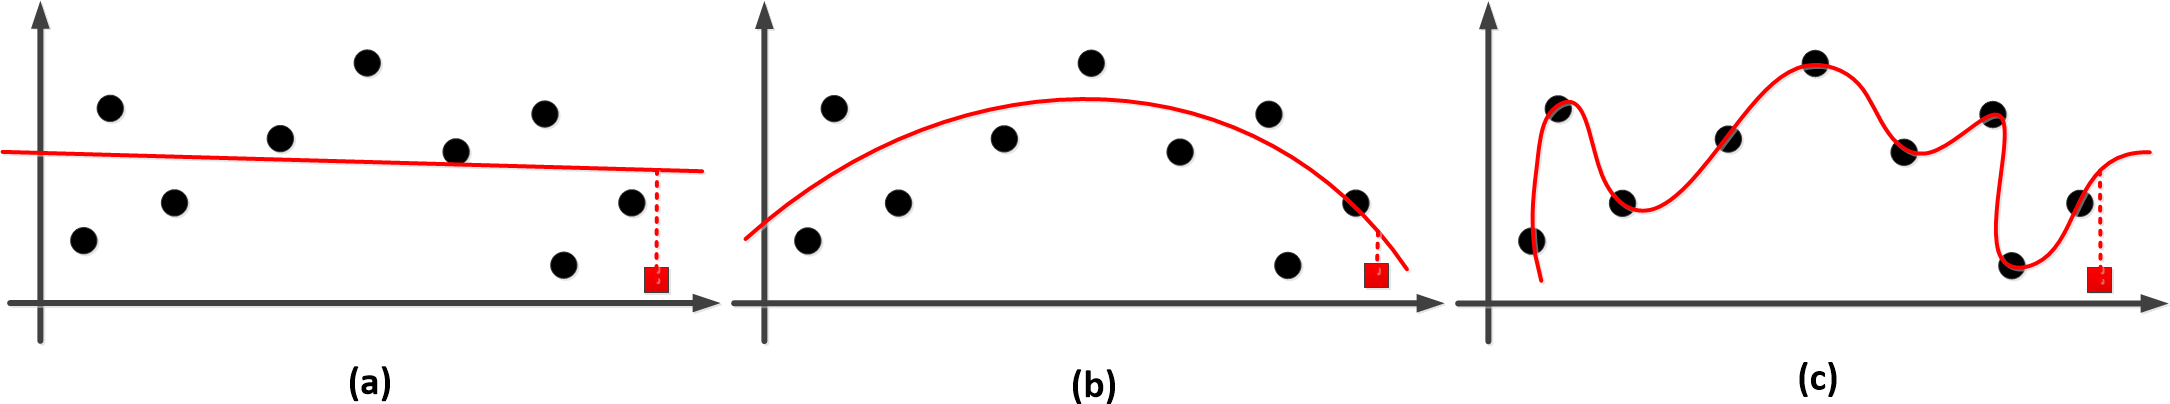
\includegraphics[width=\linewidth]{media/networkquality.png}
  \caption{Visualization of different qualities of network fits \cite{underfit}. The red line represents the data fit that was generated during training. The black dots symbolize the training samples and the red square denotes a validation sample. In the first example \textbf{(a)}, the network doesn't fit the training data well, such that the network prediction of the validation sample indicated by the meeting point of the dashed and solid red line is far away from the prediction target. Such a network would not qualify for evaluation. In the second example \textbf{(b)}, the network fits the data well, such that the prediction is close to the target. This network would meet the quality requirement. In the last example \textbf{(c)}, the network fits the training data too well, such that the prediction for the validation target is too unrealistic. This network would not meet the quality requirements.}
  \label{fig:fitting}
\end{figure}

After checking the quality of a network, we can then feed \textit{evaluation data} with unknown prediction targets into the network and gain a network prediction.

\subsection{Structure and Mathematical Framework}

\begin{wrapfigure}{r}{5cm}
  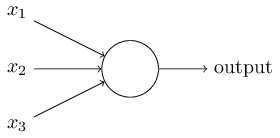
\includegraphics[width=5cm]{media/neuron.png}
  \caption{
    An example neuron with three input connections $x_1$, $x_2$ and
    $x_3$ and an output connection. \cite{nielsen}
  }
  \label{fig:neuron}
\end{wrapfigure}
To understand how an artificial neural network processes large amounts of data,
we must first discuss the structure of such networks.

In an ANN, the basic data processing unit is a neuron. Its only job is to take
input signals from directed connections to other neurons and process these inputs to generate an output signal, which can itself be connected to the input of other neurons. In \autoref{fig:neuron}, a sample neuron is depicted.

The activation $a$ of a neuron is computed by adding the input signals $x_j$ multiplied with connection weights $w_j$, representing the strength of the connection. This weighted sum is then added to a neuron bias $b$ and normalized using an activation function $\sigma$, yielding

\begin{equation}
  a = \sigma\left(\sum_j w_j x_j + b\right).
\end{equation}
In most use-cases, the activation function $\sigma$ is chosen such that the
neuron outputs are restricted to subsets of $\R$. To force neuron activations
to lie in $(0,1)$, one can use the sigmoid function
$\sigma(z) = [1+\exp(-z)]^{-1}$.

In feedforward neural networks, neurons are organized in layers 1 to $N$.
In each layer $n$, there are $L^{(n)}$ neurons and the neurons have an outbound connection to every neuron in layer $n+1$.
The $L^{(1)}$ neurons of layer 1 have no input connections and can be used to directly feed $L^{(1)}$-dimensional input data to the network.
The first layer of a neural network is thus called the \textit{input layer}.
When we feed $L^{(1)}$-dimensional data into the network, it propagates forward, layer-by-layer until the last layer, where the activations can be viewed as the processed output of the network. The last layer is thus called the \textit{output layer}.
The layers between the input and the output layer are called \textit{hidden layers}, since the activation of those neurons are neither direct inputs nor outputs of the data processing. In \autoref{fig:nn}, we can see a sample feed forward neural network.

\begin{figure}[H]
  \centering
  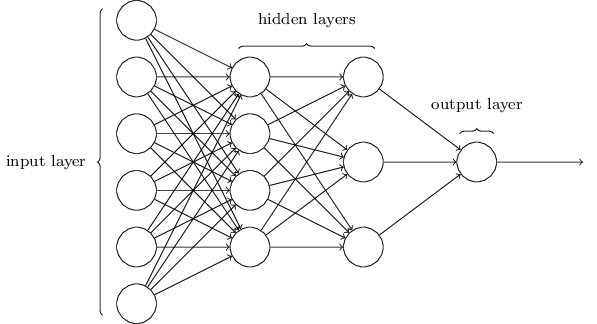
\includegraphics[width=0.7\textwidth]{media/network.png}
  \caption{A neural network with four layers \cite{nielsen}. Here, there are 6 neuron in the input layer ($L^{(1)} = 6$), 3 neurons in each hidden layer ($L^{(2)} = L^{(3)} = 3$) and one output neuron in the output layer ($L^{(4)}=1$). The connection between the neurons are limited to adjacent layers and information is only flowing from left to right. The depicted network is thus a feedforward network.}
  \label{fig:nn}
\end{figure}

Now, let $\vec{a}^{(n)} = (a_1, a_2, \dotsb, a_{L^{(n)}}) \in \R^{L^{(n)}}$ be the activations and $\vec{b}^{(n)} = (b_1, b_2, \dotsb, b_{L^{(n)}}) \in \R^{L^{(n)}}$ be the biases of the neurons in Layer $n$. For $1< n < N$, the activation of the neurons in layer $n+1$ can be functionally described by
\begin{align}
  A^{(n)}: \R^{L^{(n)}} & \longmapsto \R^{L^{(n+1)}}                                                        \\
  \vec{a}^{(n)}         & \longmapsto \vec{a}^{(n+1)} = \sigma\left(W^{(n)}\vec{a}^{(n)} +b^{(n+1)}\right).
\end{align}
Here, $W^{(n)} = (w^{(n)}_{ij})$ is the $(L^{(n+1)} \times L^{(n)})$-dimensional Matrix of the weights $w^{(n)}_{ij}$ from neuron $j$ in layer $n$ to neuron $i$ in layer $n+1$. Furthermore, the activation function $\sigma$ is applied elementwise. In that sense, one can view a neural network as a function
\begin{align}
  \label{eqn:ann_function}
  f: \R^{L^{(1)}} & \longmapsto \R^{L^{(N)}}                                                           \\
  x               & \longmapsto \left(A^{(N-1)} \circ \dotsb \circ A^{(2)}\right)(W^{(1)}x + b^{(2)}).
\end{align}
Before one constructs a feedforward artificial neural network, one has to think about the structure (i.e the count of layers and the count of neurons in each layer) and the used activation function. Those values have to be chosen such that the network can fulfill the data requirements and output the right data.

For example, if one uses an ANN to classify greyscale images of pixel-size $24\times 24$ into two classes $A$ and $B$ (this is called a \textit{binary classification problem}), one could choose $L^{(1)} = 24 \cdot 24 = 576$ and $L^{(N)} = 2$, such that each greyscale value can be fed into one input neuron and each output neuron corresponds to one of the two classes $A$ and $B$. If one restricts the output neurons to the range $(0, 1)$, one could extract the prediction of the network by choosing the neuron with the highest activation.
% Absatz über underfitting / overfitting

The function \eqref{eqn:ann_function} is dependent on the weights and biases of the connections and neurons. They can be viewed as internal parameters of $f$. When the network is initialized, they are often set to random values and the network will output random data. The challenge of machine learning is to apply algorithms on the outputs of the network to carefully adjust the weights and biases which results in the optimization of the network model \cite{nielsen}.

\subsection{Learning Process of a network}
\label{sec:sgd}
There are many ways to tackle the optimization process of neural networks. Training methods all rely on evaluating the outputs of some given inputs and comparing them to the values that \textit{should} be output by the network.

To quantify the performance of a given network $f$, we define a \textit{loss function} which depends on given inputs $x_1, x_2, \dots, x_n \in \R^{L^{(1)}}$, their desired outputs $o_1, o_2, \dots, o_n \in \R^{L^{(N)}}$ and, most importantly, the weights $w$ and the biases $b$ of the network, by
\begin{equation}
  \label{eqn:mseloss}
  C(w, b) = \frac{1}{n}\sum_{i=1}^{n}\norm{f(x_i)-o_i}^2.
\end{equation}
Note that the loss function is always positive and only zero, when the network predicts the correct output for every input. There are many ways to choose a loss function that has these properties. The function \eqref{eqn:mseloss} is called the \textit{mean squared error} (MSE) and is used throughout this thesis as the loss function.

Using this terminology, we can translate the optimization process of a network to a well-posed problem of finding the minimum of a function. Usually, the number of dimensions is too high to compute the minimum of the loss function analytically. One has to rely on numerical methods to find a local minimum of \eqref{eqn:mseloss}. A basic numerical algorithm that is used in machine learning is called \textit{gradient descent}. Even though this algorithm is very simplistic, it provides the basis for more sophisticated optimization algorithms such as the \textit{AdamW algorithm}, which is used in this thesis.

The gradient descend method is an iterative method that can be used to find a local minimum of an arbitrary differentiable function $f: \R^n \mapsto \R, x \mapsto f(x)$. Starting from a point $x^{(0)} \in \R^n$, we iteratively adjust the value by a finite amount $\Delta x$. The function will change by
\begin{equation}
  \label{eqn:approx}
  \Delta f \approx \frac{\partial f}{\partial x_1} \Delta x_1 + \dots + \frac{\partial f}{\partial x_2} \Delta x_2 = (\nabla f)(x) \cdot \Delta x.
\end{equation}

If we choose $\Delta x = -\eta (\nabla f)(x)$, with a small positive parameter $\eta$ called the \textit{learning rate}, we can force the right hand side of \eqref{eqn:approx} to be negative. In that way, if we adjust $x$ by $\Delta x$, we can ensure that the new function value at $x^{(1)} = x^{(0)}+ \Delta x$ will be smaller, if the approximation in \eqref{eqn:approx} is good enough. For that, it is important to carefully choose the value of $\eta$ small enough, but not too small. If the step size is too small, the new value will not have changed much and the total amount of steps must be increased to obtain a reasonable optimization.

Applied to the loss function \eqref{eqn:mseloss}, we get the iteration rule
\begin{align}
  w_i & \mapsto w_i' = w_i - \eta \frac{\partial C}{\partial w_i}, \\
  b_i & \mapsto b_i' = b_i - \eta \frac{\partial C}{\partial b_i}.
\end{align}

Since the cost function depends on every input $x_i$, it is computationally infeasible to calculate the gradient of the loss function directly. Therefore, we employ the \textit{stochastic gradient descent} algorithm. The idea is to approximate the gradient of the loss function by dividing the sample set into batches and calculating the gradient only using a single batch of samples. The resulting gradient will be used to adjust the weights and biases. This allows for more steps to be taken with a single iteration over the training data set, but the steps themselves are not as accurate as with gradient descent. An iteration over the whole training data set is commonly called an \textit{epoch}. The training of a single network can be done by specifying a total amount of training \textit{epochs}, or by specifying a \textit{threshold} for the loss function for when the training should end.

To compute the gradient of the loss function for a single training sample $x$, a classical backpropagation algorithm is used. The derivative of the loss function
\begin{equation}
  \label{eqn:singleloss}
  C_x(w, b) = \norm{a_i^{(N)}-o_i}^2
\end{equation}
with respect to a weight $w_{ij}^{(N-1)}$ from the $j$-th neuron in the second last layer to the $i$-th neuron in the last layer is calculated using the chain rule to
\begin{equation}
  \frac{\partial C_x}{\partial w_{ij}^{(N-1)}} = \frac{\partial C}{\partial a_i^{(N)}}\frac{\partial a_i^{(N)}}{\partial z_i^{(N)}} \frac{\partial z_i^{(N)}}{\partial w_{ij}^{(N-1)}},
\end{equation}
where $z_i^{(n)} = \sum_{j=1} w_{ij}^{(n-1)}a_j^{(n-1)}+b_i^{(n)}$ is the activation of neuron $i$ in layer $n$ before it is fed into the activation function. Using the Loss function from \eqref{eqn:singleloss}, we get
\begin{equation}
  \frac{\partial C_x}{\partial w_{ij}^{(N-1)}} = 2(a_i^{(N)}-o_i^{(N)}) \cdot \sigma'(z_i^{(N)}) \cdot a_j^{(N-1)}.
\end{equation}
Analogously, the derivative of $C_x$ with respect to the bias $b_i^{(N)}$ is given by
\begin{equation}
  \frac{\partial C_x}{\partial b_i^{(N)}} = 2(a_i^{(N)}-o_i^{(N)}) \cdot \sigma'(z_i^{(N)}).
\end{equation}
These equations can be used to adjust the weights of the second last layer, as well as the biases of the last. Since we also need the derivative with respect to weights and biases in the earlier layers, we can use the clever trick of applying this step iteratively to one layer backwards at a time. This is why this algorithm is called backpropagation. To compute those derivatives, we need to know how the loss function changes if activations in the second last layer change. This is given by
\begin{equation}
  \frac{\partial C_x}{\partial a_j^{(N-1)}} =\sum_{i=1}^{L^{N}} 2(a_i^{(N)}-o_i^{(N)}) \cdot \sigma'(z_i^{(N)}) \cdot w_{ij}^{(N-1)}.
\end{equation}
We can use this derivative to calculate derivatives of the loss function with respect to earlier layers and iteratively determine the gradient of $C_x$. The gradient of the whole loss function $C$ is then given by the average
\begin{equation}
  \nabla C = \sum_{x} \nabla C_x
\end{equation}
over all training samples in the batch \cite{nielsen}.




\chapter{Framework}
\label{chap:framework}
\IMRADlabel{methods}
The ground-state energy sequences of NCSM calculations can show different convergence rates depending on the nucleus. For lighter nuclei, it is computationally feasible to calculate these energy sequences to a high value of $N_\mathrm{max}$, such that the clear convergence to the actual ground-state energy can be seen. For heavier nuclei, the extension of the model-space for NCSM calculations to a higher $N_\mathrm{max}$ results in the need of much more compuational power, since there are more possibilities to distribute the $N_\mathrm{max}$ excitation quanta to the nucleons. Therefore, NCSM calculations of heavier nuclei are restricted to model-spaces of lower $N_\mathrm{max}$, such that the resulting energy sequences won't show a satisfactory convergence to extract the exact ground-state energy of the nucleus given the used model of the interactions. For those cases, we need a ready-to-use extrapolation method, which should provide an estimate and its uncertainty of ground-state energy given those unconverged sequences.

The aim of this thesis is to provide an extrapolation framework for ground-state energy sequences resulting from NCSM calculations using neural networks. In order to use neural networks to extrapolate energies from unconverged sequences, we must first train the network on selected training data. In this chapter, we describe the whole workflow of training and evaluating a network, as well as a state-of-the-art extrapolation method using exponential function fits which will later be used to roughly assess the quality of the new extrapolation methods.

\section{Training Process}
Before we introduce the complete workflow to train a network on NCSM ground-state energy sequences, we first have to decide on the network structure to use.
This includes the structure of the input layer, the structure of the output layer, as well as the structure of the hidden layers.

\subsection{Network structure}
NCSM calculations are usually done with multiple different oscillator frequencies $\hbar \Omega$. Different oscillator frequencies result in different convergence rates of the energy sequences, but the limit stays the same. Thus, we want to incorporate more then one frequency into the extrapolation in order to give the maximum amount of information about the interaction and the nucleus into the network.
For that, we do not only try to extrapolate a single energy sequence, but input multiple sequences for different oscillator frequencies into the network.
We decide on 3 energy sequences with given frequencies to input into the network.

In order to determine the structure of the input layer, we must further choose a fixed length of the energy sequences which are put into the network.
For NCSM calculations for heavier nuclei, there are not many $N_\mathrm{max}$ values available, which means that we have to intentionally keep the sequence length small enough.
We decide on energy sequences of length 4.
In summary, the input layer thus has to consist of $L^{(1)} = 3\times 4 = 12$ input neurons.

Since the output of the neural network should be a single real number indicating the extrapolated ground-state energy, the output layer consists of $L^{(N)} = 1$ neuron.

For the hidden layers, there is no generally accepted method of defining the most efficient structure. For the most part, the count of the hidden layers as well as the count of the neurons in those layers have to be chosen empirically, such that the network neither underfits nor overfits the data. For our framework, we choose $N = 4$ total layers, such that there are two hidden layers of $L^{(2)} = 24$ and $L^{(3)} = 12$ neurons.

% Activation Function
Each layer besides the output layer will be given a \textit{rectifier} activation function (\textit{ReLU}) given by
\begin{equation}
  \sigma(z) = \max(0, z),
\end{equation}
which restricts the activations of the neurons to be positive. This function is chosen because it empirically yields the best results for the extrapolation. Furthermore, it simplifies the calculations on the neural network and with it the computation time. Notice that the activations of the last layer will not get rectified, as the extrapolations, and therefore the network output, should not be limited to positive ground-state energies. As a consequence, the connections of the second-last layer to the last layer will also be responsible for the sign of the extrapolated energy. In \autoref{fig:dataflow}, the data flow of our extrapolation framework is shown.


\begin{figure}[H]
  \centering
  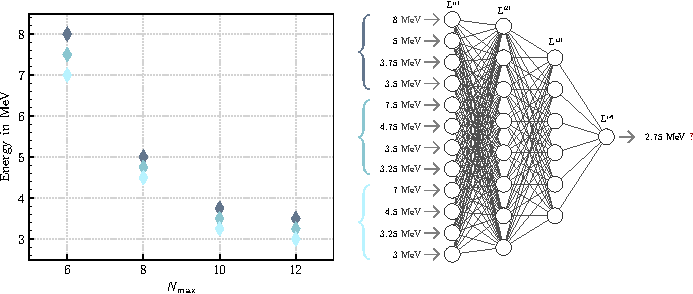
\includegraphics[width=\textwidth]{media/netviz.pdf}
  \caption{Our extrapolation framework visualized. On the left, an examplary formatted input is shown, consisting of three sequences of four nmax values. The data is input into the network, which then outputs an estimation on the common sequence limit. Note that not all neuron in layers $L^{(2)}$ and $L^{(3)}$ are shown for the sake of visibility. In our framework, $L^{(2)} = 24$ and $L^{(3)} = 12$.}
  \label{fig:dataflow}
\end{figure}
% Loss function
\subsection{Other parameters}
The loss function of our network is a standard \textit{Mean Squared Error} (MSE) loss given for a single network input $x$ by
\begin{equation}
  C_x = \norm{f(x)-o}^2,
\end{equation}
where $f(x)$ is the vector of activations of the neurons in the output layer given the input of $x$, and $o$ is the vector of desired activations. The unit of the loss function is therefore $\si[]{\mega\electronvolt\squared}$. For $n$ input samples $x_i$ with desired outputs $o_i$, the loss is averaged over all samples yielding
\begin{equation}
  C = \frac{1}{n}\sum_{i=1}^n C_{x_i}=\frac{1}{n} \sum_{i=1}^{n}\norm{f(x_i)-o_i}^2.
\end{equation}

% Optimization algorithm
For the optimization process, we opt for the \textit{AdamW} algorithm. This is a variant of the \textit{Adam} algorithm \cite{adamw, adam}, which is based on the simple stochastic gradient descent algorithm introduced in \autoref{sec:sgd}. As such, the general optimization process is the same as with stochastic gradient descent.

For gradient-based optimization algorithms, we have to choose a learning rate $\eta$, which determines the ratio of the step size to the value of the gradient. Too large values of $\eta$ result in the instability of the optimization algorithm, while too small values result in smaller step sizes. The learning rate is empirically chosen to be $\eta = 0.01$, such that both extreme cases will be avoided.

Overall, we iterate 20 times (\textit{epochs}) over the training data set, using batch sizes of 512. Since the learning rate can independently be adjusted for each epoch, it is common practice to reduce the learning rate once the optimization has stagnated, such that further optimization may be achieved. In out network training, we decrease the learning rate by a factor of 2, if the loss function as measured by a small set of input data called the \textit{development set} does not decrease by 10\% over 2 epochs (This mechanism is called \textit{learning rate scheduling}).

After the optimization is done, the network is validated using a \textit{validation set}. Here, the loss is computed using all samples in the validation set and compared to a threshold of \SI{0.3}{\mega\electronvolt\squared}. It the loss is smaller than the threshold, the network is suited for our extrapolation. Else, the network will be discarded.

% Implementation
To implement the neural network, we use \textit{pytorch}, which is a machine learning library for Python.

\subsection{Preparation of input data for the training process}
The networks have to be trained using energy sequences with known limits. Since it is impossible to calculate the limit using the full Hilbert space, we have to base the training on NCSM sequences which can be calculated to a sufficiently large value of $N_\mathrm{max}$, such that the lowest value for the highest $N_\mathrm{max}$ gives a good enough approximate for the limit. For that, we need to assume that the sequences have more or less converged to the limit. For the training, we thus use NCSM calculations from the nuclei \n{2}{H}, \n{3}{H} and \n{4}{He}. The interactions used are chiral two-body and three-body interactions.

% Generation of input data / Explain inflate
From the NCSM energy sequences, we first generate a large pool of input data which is formatted such that it can be input into the networks. This is necessary since NCSM energy sequences are generally calculated from more than three oscillator frequencies and more values of $N_\mathrm{max}$.

To generate formatted input sequences, we first purge a few exotic cases from the raw input data. Since oscillator frequencies of too high or too low values result in very slow-to-converge sequences, we restrict the data of the training process to oscillator frequencies between $\hbar\Omega=\SI{12}{\mega\electronvolt}$ and $\hbar\Omega=\SI{32}{\mega\electronvolt}$. Furthermore, we discard every NCSM calculation done for $N_\mathrm{max} = 0$, since they can result in unphysical energy values. For each nucleus and interaction, we also discard sequences for which the difference between the energy value for the highest $N_\mathrm{max}$ and the limit is higher than \SI{0.05}{\mega\electronvolt} to rule out further special sequences that do not converge enough to the desired limit.
In \autoref{fig:trainingseq}, an example \textit{raw} NCSM calculation is shown, using an SRG evolved Hamiltonian based on the \textit{chi2bM3A} interaction of the \n{2}{H} nucleus. The flow parameter is given by $\SI{0.04}{\femto\metre^4}$. This is an example of a calculation, which is suitable for training, since the calculations were done for sufficiently large $N_\mathrm{max}$ and the limit could be extracted. We can see the convergence for higher $N_\mathrm{max}$ to a value independent on the oscillator frequency.

\begin{figure}[H]
  \centering
  %% Creator: Matplotlib, PGF backend
%%
%% To include the figure in your LaTeX document, write
%%   \input{<filename>.pgf}
%%
%% Make sure the required packages are loaded in your preamble
%%   \usepackage{pgf}
%%
%% Figures using additional raster images can only be included by \input if
%% they are in the same directory as the main LaTeX file. For loading figures
%% from other directories you can use the `import` package
%%   \usepackage{import}
%%
%% and then include the figures with
%%   \import{<path to file>}{<filename>.pgf}
%%
%% Matplotlib used the following preamble
%%   \usepackage{fontspec}
%%   \setmainfont{DejaVuSerif.ttf}[Path=\detokenize{/home/agelmarc/.local/lib/python3.8/site-packages/matplotlib/mpl-data/fonts/ttf/}]
%%   \setsansfont{DejaVuSans.ttf}[Path=\detokenize{/home/agelmarc/.local/lib/python3.8/site-packages/matplotlib/mpl-data/fonts/ttf/}]
%%   \setmonofont{DejaVuSansMono.ttf}[Path=\detokenize{/home/agelmarc/.local/lib/python3.8/site-packages/matplotlib/mpl-data/fonts/ttf/}]
%%
\begingroup%
\makeatletter%
\begin{pgfpicture}%
\pgfpathrectangle{\pgfpointorigin}{\pgfqpoint{6.724074in}{3.505754in}}%
\pgfusepath{use as bounding box, clip}%
\begin{pgfscope}%
\pgfsetbuttcap%
\pgfsetmiterjoin%
\definecolor{currentfill}{rgb}{1.000000,1.000000,1.000000}%
\pgfsetfillcolor{currentfill}%
\pgfsetlinewidth{0.000000pt}%
\definecolor{currentstroke}{rgb}{1.000000,1.000000,1.000000}%
\pgfsetstrokecolor{currentstroke}%
\pgfsetdash{}{0pt}%
\pgfpathmoveto{\pgfqpoint{0.000000in}{0.000000in}}%
\pgfpathlineto{\pgfqpoint{6.724074in}{0.000000in}}%
\pgfpathlineto{\pgfqpoint{6.724074in}{3.505754in}}%
\pgfpathlineto{\pgfqpoint{0.000000in}{3.505754in}}%
\pgfpathclose%
\pgfusepath{fill}%
\end{pgfscope}%
\begin{pgfscope}%
\pgfsetbuttcap%
\pgfsetmiterjoin%
\definecolor{currentfill}{rgb}{1.000000,1.000000,1.000000}%
\pgfsetfillcolor{currentfill}%
\pgfsetlinewidth{0.000000pt}%
\definecolor{currentstroke}{rgb}{0.000000,0.000000,0.000000}%
\pgfsetstrokecolor{currentstroke}%
\pgfsetstrokeopacity{0.000000}%
\pgfsetdash{}{0pt}%
\pgfpathmoveto{\pgfqpoint{0.524074in}{0.372992in}}%
\pgfpathlineto{\pgfqpoint{6.724074in}{0.372992in}}%
\pgfpathlineto{\pgfqpoint{6.724074in}{3.452992in}}%
\pgfpathlineto{\pgfqpoint{0.524074in}{3.452992in}}%
\pgfpathclose%
\pgfusepath{fill}%
\end{pgfscope}%
\begin{pgfscope}%
\pgfpathrectangle{\pgfqpoint{0.524074in}{0.372992in}}{\pgfqpoint{6.200000in}{3.080000in}}%
\pgfusepath{clip}%
\pgfsetbuttcap%
\pgfsetroundjoin%
\pgfsetlinewidth{0.803000pt}%
\definecolor{currentstroke}{rgb}{0.827451,0.827451,0.827451}%
\pgfsetstrokecolor{currentstroke}%
\pgfsetdash{{0.800000pt}{1.320000pt}}{0.000000pt}%
\pgfpathmoveto{\pgfqpoint{0.524074in}{0.372992in}}%
\pgfpathlineto{\pgfqpoint{0.524074in}{3.452992in}}%
\pgfusepath{stroke}%
\end{pgfscope}%
\begin{pgfscope}%
\pgfsetbuttcap%
\pgfsetroundjoin%
\definecolor{currentfill}{rgb}{0.000000,0.000000,0.000000}%
\pgfsetfillcolor{currentfill}%
\pgfsetlinewidth{0.803000pt}%
\definecolor{currentstroke}{rgb}{0.000000,0.000000,0.000000}%
\pgfsetstrokecolor{currentstroke}%
\pgfsetdash{}{0pt}%
\pgfsys@defobject{currentmarker}{\pgfqpoint{0.000000in}{0.000000in}}{\pgfqpoint{0.000000in}{0.048611in}}{%
\pgfpathmoveto{\pgfqpoint{0.000000in}{0.000000in}}%
\pgfpathlineto{\pgfqpoint{0.000000in}{0.048611in}}%
\pgfusepath{stroke,fill}%
}%
\begin{pgfscope}%
\pgfsys@transformshift{0.524074in}{0.372992in}%
\pgfsys@useobject{currentmarker}{}%
\end{pgfscope}%
\end{pgfscope}%
\begin{pgfscope}%
\definecolor{textcolor}{rgb}{0.000000,0.000000,0.000000}%
\pgfsetstrokecolor{textcolor}%
\pgfsetfillcolor{textcolor}%
\pgftext[x=0.524074in,y=0.324381in,,top]{\color{textcolor}\fontsize{10.000000}{12.000000}\selectfont \(\displaystyle {0}\)}%
\end{pgfscope}%
\begin{pgfscope}%
\pgfpathrectangle{\pgfqpoint{0.524074in}{0.372992in}}{\pgfqpoint{6.200000in}{3.080000in}}%
\pgfusepath{clip}%
\pgfsetbuttcap%
\pgfsetroundjoin%
\pgfsetlinewidth{0.803000pt}%
\definecolor{currentstroke}{rgb}{0.827451,0.827451,0.827451}%
\pgfsetstrokecolor{currentstroke}%
\pgfsetdash{{0.800000pt}{1.320000pt}}{0.000000pt}%
\pgfpathmoveto{\pgfqpoint{1.739760in}{0.372992in}}%
\pgfpathlineto{\pgfqpoint{1.739760in}{3.452992in}}%
\pgfusepath{stroke}%
\end{pgfscope}%
\begin{pgfscope}%
\pgfsetbuttcap%
\pgfsetroundjoin%
\definecolor{currentfill}{rgb}{0.000000,0.000000,0.000000}%
\pgfsetfillcolor{currentfill}%
\pgfsetlinewidth{0.803000pt}%
\definecolor{currentstroke}{rgb}{0.000000,0.000000,0.000000}%
\pgfsetstrokecolor{currentstroke}%
\pgfsetdash{}{0pt}%
\pgfsys@defobject{currentmarker}{\pgfqpoint{0.000000in}{0.000000in}}{\pgfqpoint{0.000000in}{0.048611in}}{%
\pgfpathmoveto{\pgfqpoint{0.000000in}{0.000000in}}%
\pgfpathlineto{\pgfqpoint{0.000000in}{0.048611in}}%
\pgfusepath{stroke,fill}%
}%
\begin{pgfscope}%
\pgfsys@transformshift{1.739760in}{0.372992in}%
\pgfsys@useobject{currentmarker}{}%
\end{pgfscope}%
\end{pgfscope}%
\begin{pgfscope}%
\definecolor{textcolor}{rgb}{0.000000,0.000000,0.000000}%
\pgfsetstrokecolor{textcolor}%
\pgfsetfillcolor{textcolor}%
\pgftext[x=1.739760in,y=0.324381in,,top]{\color{textcolor}\fontsize{10.000000}{12.000000}\selectfont \(\displaystyle {10}\)}%
\end{pgfscope}%
\begin{pgfscope}%
\pgfpathrectangle{\pgfqpoint{0.524074in}{0.372992in}}{\pgfqpoint{6.200000in}{3.080000in}}%
\pgfusepath{clip}%
\pgfsetbuttcap%
\pgfsetroundjoin%
\pgfsetlinewidth{0.803000pt}%
\definecolor{currentstroke}{rgb}{0.827451,0.827451,0.827451}%
\pgfsetstrokecolor{currentstroke}%
\pgfsetdash{{0.800000pt}{1.320000pt}}{0.000000pt}%
\pgfpathmoveto{\pgfqpoint{2.955447in}{0.372992in}}%
\pgfpathlineto{\pgfqpoint{2.955447in}{3.452992in}}%
\pgfusepath{stroke}%
\end{pgfscope}%
\begin{pgfscope}%
\pgfsetbuttcap%
\pgfsetroundjoin%
\definecolor{currentfill}{rgb}{0.000000,0.000000,0.000000}%
\pgfsetfillcolor{currentfill}%
\pgfsetlinewidth{0.803000pt}%
\definecolor{currentstroke}{rgb}{0.000000,0.000000,0.000000}%
\pgfsetstrokecolor{currentstroke}%
\pgfsetdash{}{0pt}%
\pgfsys@defobject{currentmarker}{\pgfqpoint{0.000000in}{0.000000in}}{\pgfqpoint{0.000000in}{0.048611in}}{%
\pgfpathmoveto{\pgfqpoint{0.000000in}{0.000000in}}%
\pgfpathlineto{\pgfqpoint{0.000000in}{0.048611in}}%
\pgfusepath{stroke,fill}%
}%
\begin{pgfscope}%
\pgfsys@transformshift{2.955447in}{0.372992in}%
\pgfsys@useobject{currentmarker}{}%
\end{pgfscope}%
\end{pgfscope}%
\begin{pgfscope}%
\definecolor{textcolor}{rgb}{0.000000,0.000000,0.000000}%
\pgfsetstrokecolor{textcolor}%
\pgfsetfillcolor{textcolor}%
\pgftext[x=2.955447in,y=0.324381in,,top]{\color{textcolor}\fontsize{10.000000}{12.000000}\selectfont \(\displaystyle {20}\)}%
\end{pgfscope}%
\begin{pgfscope}%
\pgfpathrectangle{\pgfqpoint{0.524074in}{0.372992in}}{\pgfqpoint{6.200000in}{3.080000in}}%
\pgfusepath{clip}%
\pgfsetbuttcap%
\pgfsetroundjoin%
\pgfsetlinewidth{0.803000pt}%
\definecolor{currentstroke}{rgb}{0.827451,0.827451,0.827451}%
\pgfsetstrokecolor{currentstroke}%
\pgfsetdash{{0.800000pt}{1.320000pt}}{0.000000pt}%
\pgfpathmoveto{\pgfqpoint{4.171133in}{0.372992in}}%
\pgfpathlineto{\pgfqpoint{4.171133in}{3.452992in}}%
\pgfusepath{stroke}%
\end{pgfscope}%
\begin{pgfscope}%
\pgfsetbuttcap%
\pgfsetroundjoin%
\definecolor{currentfill}{rgb}{0.000000,0.000000,0.000000}%
\pgfsetfillcolor{currentfill}%
\pgfsetlinewidth{0.803000pt}%
\definecolor{currentstroke}{rgb}{0.000000,0.000000,0.000000}%
\pgfsetstrokecolor{currentstroke}%
\pgfsetdash{}{0pt}%
\pgfsys@defobject{currentmarker}{\pgfqpoint{0.000000in}{0.000000in}}{\pgfqpoint{0.000000in}{0.048611in}}{%
\pgfpathmoveto{\pgfqpoint{0.000000in}{0.000000in}}%
\pgfpathlineto{\pgfqpoint{0.000000in}{0.048611in}}%
\pgfusepath{stroke,fill}%
}%
\begin{pgfscope}%
\pgfsys@transformshift{4.171133in}{0.372992in}%
\pgfsys@useobject{currentmarker}{}%
\end{pgfscope}%
\end{pgfscope}%
\begin{pgfscope}%
\definecolor{textcolor}{rgb}{0.000000,0.000000,0.000000}%
\pgfsetstrokecolor{textcolor}%
\pgfsetfillcolor{textcolor}%
\pgftext[x=4.171133in,y=0.324381in,,top]{\color{textcolor}\fontsize{10.000000}{12.000000}\selectfont \(\displaystyle {30}\)}%
\end{pgfscope}%
\begin{pgfscope}%
\pgfpathrectangle{\pgfqpoint{0.524074in}{0.372992in}}{\pgfqpoint{6.200000in}{3.080000in}}%
\pgfusepath{clip}%
\pgfsetbuttcap%
\pgfsetroundjoin%
\pgfsetlinewidth{0.803000pt}%
\definecolor{currentstroke}{rgb}{0.827451,0.827451,0.827451}%
\pgfsetstrokecolor{currentstroke}%
\pgfsetdash{{0.800000pt}{1.320000pt}}{0.000000pt}%
\pgfpathmoveto{\pgfqpoint{5.386819in}{0.372992in}}%
\pgfpathlineto{\pgfqpoint{5.386819in}{3.452992in}}%
\pgfusepath{stroke}%
\end{pgfscope}%
\begin{pgfscope}%
\pgfsetbuttcap%
\pgfsetroundjoin%
\definecolor{currentfill}{rgb}{0.000000,0.000000,0.000000}%
\pgfsetfillcolor{currentfill}%
\pgfsetlinewidth{0.803000pt}%
\definecolor{currentstroke}{rgb}{0.000000,0.000000,0.000000}%
\pgfsetstrokecolor{currentstroke}%
\pgfsetdash{}{0pt}%
\pgfsys@defobject{currentmarker}{\pgfqpoint{0.000000in}{0.000000in}}{\pgfqpoint{0.000000in}{0.048611in}}{%
\pgfpathmoveto{\pgfqpoint{0.000000in}{0.000000in}}%
\pgfpathlineto{\pgfqpoint{0.000000in}{0.048611in}}%
\pgfusepath{stroke,fill}%
}%
\begin{pgfscope}%
\pgfsys@transformshift{5.386819in}{0.372992in}%
\pgfsys@useobject{currentmarker}{}%
\end{pgfscope}%
\end{pgfscope}%
\begin{pgfscope}%
\definecolor{textcolor}{rgb}{0.000000,0.000000,0.000000}%
\pgfsetstrokecolor{textcolor}%
\pgfsetfillcolor{textcolor}%
\pgftext[x=5.386819in,y=0.324381in,,top]{\color{textcolor}\fontsize{10.000000}{12.000000}\selectfont \(\displaystyle {40}\)}%
\end{pgfscope}%
\begin{pgfscope}%
\pgfpathrectangle{\pgfqpoint{0.524074in}{0.372992in}}{\pgfqpoint{6.200000in}{3.080000in}}%
\pgfusepath{clip}%
\pgfsetbuttcap%
\pgfsetroundjoin%
\pgfsetlinewidth{0.803000pt}%
\definecolor{currentstroke}{rgb}{0.827451,0.827451,0.827451}%
\pgfsetstrokecolor{currentstroke}%
\pgfsetdash{{0.800000pt}{1.320000pt}}{0.000000pt}%
\pgfpathmoveto{\pgfqpoint{6.602506in}{0.372992in}}%
\pgfpathlineto{\pgfqpoint{6.602506in}{3.452992in}}%
\pgfusepath{stroke}%
\end{pgfscope}%
\begin{pgfscope}%
\pgfsetbuttcap%
\pgfsetroundjoin%
\definecolor{currentfill}{rgb}{0.000000,0.000000,0.000000}%
\pgfsetfillcolor{currentfill}%
\pgfsetlinewidth{0.803000pt}%
\definecolor{currentstroke}{rgb}{0.000000,0.000000,0.000000}%
\pgfsetstrokecolor{currentstroke}%
\pgfsetdash{}{0pt}%
\pgfsys@defobject{currentmarker}{\pgfqpoint{0.000000in}{0.000000in}}{\pgfqpoint{0.000000in}{0.048611in}}{%
\pgfpathmoveto{\pgfqpoint{0.000000in}{0.000000in}}%
\pgfpathlineto{\pgfqpoint{0.000000in}{0.048611in}}%
\pgfusepath{stroke,fill}%
}%
\begin{pgfscope}%
\pgfsys@transformshift{6.602506in}{0.372992in}%
\pgfsys@useobject{currentmarker}{}%
\end{pgfscope}%
\end{pgfscope}%
\begin{pgfscope}%
\definecolor{textcolor}{rgb}{0.000000,0.000000,0.000000}%
\pgfsetstrokecolor{textcolor}%
\pgfsetfillcolor{textcolor}%
\pgftext[x=6.602506in,y=0.324381in,,top]{\color{textcolor}\fontsize{10.000000}{12.000000}\selectfont \(\displaystyle {50}\)}%
\end{pgfscope}%
\begin{pgfscope}%
\pgfsetbuttcap%
\pgfsetroundjoin%
\definecolor{currentfill}{rgb}{0.000000,0.000000,0.000000}%
\pgfsetfillcolor{currentfill}%
\pgfsetlinewidth{0.602250pt}%
\definecolor{currentstroke}{rgb}{0.000000,0.000000,0.000000}%
\pgfsetstrokecolor{currentstroke}%
\pgfsetdash{}{0pt}%
\pgfsys@defobject{currentmarker}{\pgfqpoint{0.000000in}{0.000000in}}{\pgfqpoint{0.000000in}{0.027778in}}{%
\pgfpathmoveto{\pgfqpoint{0.000000in}{0.000000in}}%
\pgfpathlineto{\pgfqpoint{0.000000in}{0.027778in}}%
\pgfusepath{stroke,fill}%
}%
\begin{pgfscope}%
\pgfsys@transformshift{0.767211in}{0.372992in}%
\pgfsys@useobject{currentmarker}{}%
\end{pgfscope}%
\end{pgfscope}%
\begin{pgfscope}%
\pgfsetbuttcap%
\pgfsetroundjoin%
\definecolor{currentfill}{rgb}{0.000000,0.000000,0.000000}%
\pgfsetfillcolor{currentfill}%
\pgfsetlinewidth{0.602250pt}%
\definecolor{currentstroke}{rgb}{0.000000,0.000000,0.000000}%
\pgfsetstrokecolor{currentstroke}%
\pgfsetdash{}{0pt}%
\pgfsys@defobject{currentmarker}{\pgfqpoint{0.000000in}{0.000000in}}{\pgfqpoint{0.000000in}{0.027778in}}{%
\pgfpathmoveto{\pgfqpoint{0.000000in}{0.000000in}}%
\pgfpathlineto{\pgfqpoint{0.000000in}{0.027778in}}%
\pgfusepath{stroke,fill}%
}%
\begin{pgfscope}%
\pgfsys@transformshift{1.010349in}{0.372992in}%
\pgfsys@useobject{currentmarker}{}%
\end{pgfscope}%
\end{pgfscope}%
\begin{pgfscope}%
\pgfsetbuttcap%
\pgfsetroundjoin%
\definecolor{currentfill}{rgb}{0.000000,0.000000,0.000000}%
\pgfsetfillcolor{currentfill}%
\pgfsetlinewidth{0.602250pt}%
\definecolor{currentstroke}{rgb}{0.000000,0.000000,0.000000}%
\pgfsetstrokecolor{currentstroke}%
\pgfsetdash{}{0pt}%
\pgfsys@defobject{currentmarker}{\pgfqpoint{0.000000in}{0.000000in}}{\pgfqpoint{0.000000in}{0.027778in}}{%
\pgfpathmoveto{\pgfqpoint{0.000000in}{0.000000in}}%
\pgfpathlineto{\pgfqpoint{0.000000in}{0.027778in}}%
\pgfusepath{stroke,fill}%
}%
\begin{pgfscope}%
\pgfsys@transformshift{1.253486in}{0.372992in}%
\pgfsys@useobject{currentmarker}{}%
\end{pgfscope}%
\end{pgfscope}%
\begin{pgfscope}%
\pgfsetbuttcap%
\pgfsetroundjoin%
\definecolor{currentfill}{rgb}{0.000000,0.000000,0.000000}%
\pgfsetfillcolor{currentfill}%
\pgfsetlinewidth{0.602250pt}%
\definecolor{currentstroke}{rgb}{0.000000,0.000000,0.000000}%
\pgfsetstrokecolor{currentstroke}%
\pgfsetdash{}{0pt}%
\pgfsys@defobject{currentmarker}{\pgfqpoint{0.000000in}{0.000000in}}{\pgfqpoint{0.000000in}{0.027778in}}{%
\pgfpathmoveto{\pgfqpoint{0.000000in}{0.000000in}}%
\pgfpathlineto{\pgfqpoint{0.000000in}{0.027778in}}%
\pgfusepath{stroke,fill}%
}%
\begin{pgfscope}%
\pgfsys@transformshift{1.496623in}{0.372992in}%
\pgfsys@useobject{currentmarker}{}%
\end{pgfscope}%
\end{pgfscope}%
\begin{pgfscope}%
\pgfsetbuttcap%
\pgfsetroundjoin%
\definecolor{currentfill}{rgb}{0.000000,0.000000,0.000000}%
\pgfsetfillcolor{currentfill}%
\pgfsetlinewidth{0.602250pt}%
\definecolor{currentstroke}{rgb}{0.000000,0.000000,0.000000}%
\pgfsetstrokecolor{currentstroke}%
\pgfsetdash{}{0pt}%
\pgfsys@defobject{currentmarker}{\pgfqpoint{0.000000in}{0.000000in}}{\pgfqpoint{0.000000in}{0.027778in}}{%
\pgfpathmoveto{\pgfqpoint{0.000000in}{0.000000in}}%
\pgfpathlineto{\pgfqpoint{0.000000in}{0.027778in}}%
\pgfusepath{stroke,fill}%
}%
\begin{pgfscope}%
\pgfsys@transformshift{1.982898in}{0.372992in}%
\pgfsys@useobject{currentmarker}{}%
\end{pgfscope}%
\end{pgfscope}%
\begin{pgfscope}%
\pgfsetbuttcap%
\pgfsetroundjoin%
\definecolor{currentfill}{rgb}{0.000000,0.000000,0.000000}%
\pgfsetfillcolor{currentfill}%
\pgfsetlinewidth{0.602250pt}%
\definecolor{currentstroke}{rgb}{0.000000,0.000000,0.000000}%
\pgfsetstrokecolor{currentstroke}%
\pgfsetdash{}{0pt}%
\pgfsys@defobject{currentmarker}{\pgfqpoint{0.000000in}{0.000000in}}{\pgfqpoint{0.000000in}{0.027778in}}{%
\pgfpathmoveto{\pgfqpoint{0.000000in}{0.000000in}}%
\pgfpathlineto{\pgfqpoint{0.000000in}{0.027778in}}%
\pgfusepath{stroke,fill}%
}%
\begin{pgfscope}%
\pgfsys@transformshift{2.226035in}{0.372992in}%
\pgfsys@useobject{currentmarker}{}%
\end{pgfscope}%
\end{pgfscope}%
\begin{pgfscope}%
\pgfsetbuttcap%
\pgfsetroundjoin%
\definecolor{currentfill}{rgb}{0.000000,0.000000,0.000000}%
\pgfsetfillcolor{currentfill}%
\pgfsetlinewidth{0.602250pt}%
\definecolor{currentstroke}{rgb}{0.000000,0.000000,0.000000}%
\pgfsetstrokecolor{currentstroke}%
\pgfsetdash{}{0pt}%
\pgfsys@defobject{currentmarker}{\pgfqpoint{0.000000in}{0.000000in}}{\pgfqpoint{0.000000in}{0.027778in}}{%
\pgfpathmoveto{\pgfqpoint{0.000000in}{0.000000in}}%
\pgfpathlineto{\pgfqpoint{0.000000in}{0.027778in}}%
\pgfusepath{stroke,fill}%
}%
\begin{pgfscope}%
\pgfsys@transformshift{2.469172in}{0.372992in}%
\pgfsys@useobject{currentmarker}{}%
\end{pgfscope}%
\end{pgfscope}%
\begin{pgfscope}%
\pgfsetbuttcap%
\pgfsetroundjoin%
\definecolor{currentfill}{rgb}{0.000000,0.000000,0.000000}%
\pgfsetfillcolor{currentfill}%
\pgfsetlinewidth{0.602250pt}%
\definecolor{currentstroke}{rgb}{0.000000,0.000000,0.000000}%
\pgfsetstrokecolor{currentstroke}%
\pgfsetdash{}{0pt}%
\pgfsys@defobject{currentmarker}{\pgfqpoint{0.000000in}{0.000000in}}{\pgfqpoint{0.000000in}{0.027778in}}{%
\pgfpathmoveto{\pgfqpoint{0.000000in}{0.000000in}}%
\pgfpathlineto{\pgfqpoint{0.000000in}{0.027778in}}%
\pgfusepath{stroke,fill}%
}%
\begin{pgfscope}%
\pgfsys@transformshift{2.712309in}{0.372992in}%
\pgfsys@useobject{currentmarker}{}%
\end{pgfscope}%
\end{pgfscope}%
\begin{pgfscope}%
\pgfsetbuttcap%
\pgfsetroundjoin%
\definecolor{currentfill}{rgb}{0.000000,0.000000,0.000000}%
\pgfsetfillcolor{currentfill}%
\pgfsetlinewidth{0.602250pt}%
\definecolor{currentstroke}{rgb}{0.000000,0.000000,0.000000}%
\pgfsetstrokecolor{currentstroke}%
\pgfsetdash{}{0pt}%
\pgfsys@defobject{currentmarker}{\pgfqpoint{0.000000in}{0.000000in}}{\pgfqpoint{0.000000in}{0.027778in}}{%
\pgfpathmoveto{\pgfqpoint{0.000000in}{0.000000in}}%
\pgfpathlineto{\pgfqpoint{0.000000in}{0.027778in}}%
\pgfusepath{stroke,fill}%
}%
\begin{pgfscope}%
\pgfsys@transformshift{3.198584in}{0.372992in}%
\pgfsys@useobject{currentmarker}{}%
\end{pgfscope}%
\end{pgfscope}%
\begin{pgfscope}%
\pgfsetbuttcap%
\pgfsetroundjoin%
\definecolor{currentfill}{rgb}{0.000000,0.000000,0.000000}%
\pgfsetfillcolor{currentfill}%
\pgfsetlinewidth{0.602250pt}%
\definecolor{currentstroke}{rgb}{0.000000,0.000000,0.000000}%
\pgfsetstrokecolor{currentstroke}%
\pgfsetdash{}{0pt}%
\pgfsys@defobject{currentmarker}{\pgfqpoint{0.000000in}{0.000000in}}{\pgfqpoint{0.000000in}{0.027778in}}{%
\pgfpathmoveto{\pgfqpoint{0.000000in}{0.000000in}}%
\pgfpathlineto{\pgfqpoint{0.000000in}{0.027778in}}%
\pgfusepath{stroke,fill}%
}%
\begin{pgfscope}%
\pgfsys@transformshift{3.441721in}{0.372992in}%
\pgfsys@useobject{currentmarker}{}%
\end{pgfscope}%
\end{pgfscope}%
\begin{pgfscope}%
\pgfsetbuttcap%
\pgfsetroundjoin%
\definecolor{currentfill}{rgb}{0.000000,0.000000,0.000000}%
\pgfsetfillcolor{currentfill}%
\pgfsetlinewidth{0.602250pt}%
\definecolor{currentstroke}{rgb}{0.000000,0.000000,0.000000}%
\pgfsetstrokecolor{currentstroke}%
\pgfsetdash{}{0pt}%
\pgfsys@defobject{currentmarker}{\pgfqpoint{0.000000in}{0.000000in}}{\pgfqpoint{0.000000in}{0.027778in}}{%
\pgfpathmoveto{\pgfqpoint{0.000000in}{0.000000in}}%
\pgfpathlineto{\pgfqpoint{0.000000in}{0.027778in}}%
\pgfusepath{stroke,fill}%
}%
\begin{pgfscope}%
\pgfsys@transformshift{3.684858in}{0.372992in}%
\pgfsys@useobject{currentmarker}{}%
\end{pgfscope}%
\end{pgfscope}%
\begin{pgfscope}%
\pgfsetbuttcap%
\pgfsetroundjoin%
\definecolor{currentfill}{rgb}{0.000000,0.000000,0.000000}%
\pgfsetfillcolor{currentfill}%
\pgfsetlinewidth{0.602250pt}%
\definecolor{currentstroke}{rgb}{0.000000,0.000000,0.000000}%
\pgfsetstrokecolor{currentstroke}%
\pgfsetdash{}{0pt}%
\pgfsys@defobject{currentmarker}{\pgfqpoint{0.000000in}{0.000000in}}{\pgfqpoint{0.000000in}{0.027778in}}{%
\pgfpathmoveto{\pgfqpoint{0.000000in}{0.000000in}}%
\pgfpathlineto{\pgfqpoint{0.000000in}{0.027778in}}%
\pgfusepath{stroke,fill}%
}%
\begin{pgfscope}%
\pgfsys@transformshift{3.927996in}{0.372992in}%
\pgfsys@useobject{currentmarker}{}%
\end{pgfscope}%
\end{pgfscope}%
\begin{pgfscope}%
\pgfsetbuttcap%
\pgfsetroundjoin%
\definecolor{currentfill}{rgb}{0.000000,0.000000,0.000000}%
\pgfsetfillcolor{currentfill}%
\pgfsetlinewidth{0.602250pt}%
\definecolor{currentstroke}{rgb}{0.000000,0.000000,0.000000}%
\pgfsetstrokecolor{currentstroke}%
\pgfsetdash{}{0pt}%
\pgfsys@defobject{currentmarker}{\pgfqpoint{0.000000in}{0.000000in}}{\pgfqpoint{0.000000in}{0.027778in}}{%
\pgfpathmoveto{\pgfqpoint{0.000000in}{0.000000in}}%
\pgfpathlineto{\pgfqpoint{0.000000in}{0.027778in}}%
\pgfusepath{stroke,fill}%
}%
\begin{pgfscope}%
\pgfsys@transformshift{4.414270in}{0.372992in}%
\pgfsys@useobject{currentmarker}{}%
\end{pgfscope}%
\end{pgfscope}%
\begin{pgfscope}%
\pgfsetbuttcap%
\pgfsetroundjoin%
\definecolor{currentfill}{rgb}{0.000000,0.000000,0.000000}%
\pgfsetfillcolor{currentfill}%
\pgfsetlinewidth{0.602250pt}%
\definecolor{currentstroke}{rgb}{0.000000,0.000000,0.000000}%
\pgfsetstrokecolor{currentstroke}%
\pgfsetdash{}{0pt}%
\pgfsys@defobject{currentmarker}{\pgfqpoint{0.000000in}{0.000000in}}{\pgfqpoint{0.000000in}{0.027778in}}{%
\pgfpathmoveto{\pgfqpoint{0.000000in}{0.000000in}}%
\pgfpathlineto{\pgfqpoint{0.000000in}{0.027778in}}%
\pgfusepath{stroke,fill}%
}%
\begin{pgfscope}%
\pgfsys@transformshift{4.657407in}{0.372992in}%
\pgfsys@useobject{currentmarker}{}%
\end{pgfscope}%
\end{pgfscope}%
\begin{pgfscope}%
\pgfsetbuttcap%
\pgfsetroundjoin%
\definecolor{currentfill}{rgb}{0.000000,0.000000,0.000000}%
\pgfsetfillcolor{currentfill}%
\pgfsetlinewidth{0.602250pt}%
\definecolor{currentstroke}{rgb}{0.000000,0.000000,0.000000}%
\pgfsetstrokecolor{currentstroke}%
\pgfsetdash{}{0pt}%
\pgfsys@defobject{currentmarker}{\pgfqpoint{0.000000in}{0.000000in}}{\pgfqpoint{0.000000in}{0.027778in}}{%
\pgfpathmoveto{\pgfqpoint{0.000000in}{0.000000in}}%
\pgfpathlineto{\pgfqpoint{0.000000in}{0.027778in}}%
\pgfusepath{stroke,fill}%
}%
\begin{pgfscope}%
\pgfsys@transformshift{4.900545in}{0.372992in}%
\pgfsys@useobject{currentmarker}{}%
\end{pgfscope}%
\end{pgfscope}%
\begin{pgfscope}%
\pgfsetbuttcap%
\pgfsetroundjoin%
\definecolor{currentfill}{rgb}{0.000000,0.000000,0.000000}%
\pgfsetfillcolor{currentfill}%
\pgfsetlinewidth{0.602250pt}%
\definecolor{currentstroke}{rgb}{0.000000,0.000000,0.000000}%
\pgfsetstrokecolor{currentstroke}%
\pgfsetdash{}{0pt}%
\pgfsys@defobject{currentmarker}{\pgfqpoint{0.000000in}{0.000000in}}{\pgfqpoint{0.000000in}{0.027778in}}{%
\pgfpathmoveto{\pgfqpoint{0.000000in}{0.000000in}}%
\pgfpathlineto{\pgfqpoint{0.000000in}{0.027778in}}%
\pgfusepath{stroke,fill}%
}%
\begin{pgfscope}%
\pgfsys@transformshift{5.143682in}{0.372992in}%
\pgfsys@useobject{currentmarker}{}%
\end{pgfscope}%
\end{pgfscope}%
\begin{pgfscope}%
\pgfsetbuttcap%
\pgfsetroundjoin%
\definecolor{currentfill}{rgb}{0.000000,0.000000,0.000000}%
\pgfsetfillcolor{currentfill}%
\pgfsetlinewidth{0.602250pt}%
\definecolor{currentstroke}{rgb}{0.000000,0.000000,0.000000}%
\pgfsetstrokecolor{currentstroke}%
\pgfsetdash{}{0pt}%
\pgfsys@defobject{currentmarker}{\pgfqpoint{0.000000in}{0.000000in}}{\pgfqpoint{0.000000in}{0.027778in}}{%
\pgfpathmoveto{\pgfqpoint{0.000000in}{0.000000in}}%
\pgfpathlineto{\pgfqpoint{0.000000in}{0.027778in}}%
\pgfusepath{stroke,fill}%
}%
\begin{pgfscope}%
\pgfsys@transformshift{5.629957in}{0.372992in}%
\pgfsys@useobject{currentmarker}{}%
\end{pgfscope}%
\end{pgfscope}%
\begin{pgfscope}%
\pgfsetbuttcap%
\pgfsetroundjoin%
\definecolor{currentfill}{rgb}{0.000000,0.000000,0.000000}%
\pgfsetfillcolor{currentfill}%
\pgfsetlinewidth{0.602250pt}%
\definecolor{currentstroke}{rgb}{0.000000,0.000000,0.000000}%
\pgfsetstrokecolor{currentstroke}%
\pgfsetdash{}{0pt}%
\pgfsys@defobject{currentmarker}{\pgfqpoint{0.000000in}{0.000000in}}{\pgfqpoint{0.000000in}{0.027778in}}{%
\pgfpathmoveto{\pgfqpoint{0.000000in}{0.000000in}}%
\pgfpathlineto{\pgfqpoint{0.000000in}{0.027778in}}%
\pgfusepath{stroke,fill}%
}%
\begin{pgfscope}%
\pgfsys@transformshift{5.873094in}{0.372992in}%
\pgfsys@useobject{currentmarker}{}%
\end{pgfscope}%
\end{pgfscope}%
\begin{pgfscope}%
\pgfsetbuttcap%
\pgfsetroundjoin%
\definecolor{currentfill}{rgb}{0.000000,0.000000,0.000000}%
\pgfsetfillcolor{currentfill}%
\pgfsetlinewidth{0.602250pt}%
\definecolor{currentstroke}{rgb}{0.000000,0.000000,0.000000}%
\pgfsetstrokecolor{currentstroke}%
\pgfsetdash{}{0pt}%
\pgfsys@defobject{currentmarker}{\pgfqpoint{0.000000in}{0.000000in}}{\pgfqpoint{0.000000in}{0.027778in}}{%
\pgfpathmoveto{\pgfqpoint{0.000000in}{0.000000in}}%
\pgfpathlineto{\pgfqpoint{0.000000in}{0.027778in}}%
\pgfusepath{stroke,fill}%
}%
\begin{pgfscope}%
\pgfsys@transformshift{6.116231in}{0.372992in}%
\pgfsys@useobject{currentmarker}{}%
\end{pgfscope}%
\end{pgfscope}%
\begin{pgfscope}%
\pgfsetbuttcap%
\pgfsetroundjoin%
\definecolor{currentfill}{rgb}{0.000000,0.000000,0.000000}%
\pgfsetfillcolor{currentfill}%
\pgfsetlinewidth{0.602250pt}%
\definecolor{currentstroke}{rgb}{0.000000,0.000000,0.000000}%
\pgfsetstrokecolor{currentstroke}%
\pgfsetdash{}{0pt}%
\pgfsys@defobject{currentmarker}{\pgfqpoint{0.000000in}{0.000000in}}{\pgfqpoint{0.000000in}{0.027778in}}{%
\pgfpathmoveto{\pgfqpoint{0.000000in}{0.000000in}}%
\pgfpathlineto{\pgfqpoint{0.000000in}{0.027778in}}%
\pgfusepath{stroke,fill}%
}%
\begin{pgfscope}%
\pgfsys@transformshift{6.359368in}{0.372992in}%
\pgfsys@useobject{currentmarker}{}%
\end{pgfscope}%
\end{pgfscope}%
\begin{pgfscope}%
\definecolor{textcolor}{rgb}{0.000000,0.000000,0.000000}%
\pgfsetstrokecolor{textcolor}%
\pgfsetfillcolor{textcolor}%
\pgftext[x=3.624074in,y=0.134413in,,top]{\color{textcolor}\fontsize{10.000000}{12.000000}\selectfont \(\displaystyle N_\mathrm{max}\)}%
\end{pgfscope}%
\begin{pgfscope}%
\pgfpathrectangle{\pgfqpoint{0.524074in}{0.372992in}}{\pgfqpoint{6.200000in}{3.080000in}}%
\pgfusepath{clip}%
\pgfsetbuttcap%
\pgfsetroundjoin%
\pgfsetlinewidth{0.803000pt}%
\definecolor{currentstroke}{rgb}{0.827451,0.827451,0.827451}%
\pgfsetstrokecolor{currentstroke}%
\pgfsetdash{{0.800000pt}{1.320000pt}}{0.000000pt}%
\pgfpathmoveto{\pgfqpoint{0.524074in}{0.609915in}}%
\pgfpathlineto{\pgfqpoint{6.724074in}{0.609915in}}%
\pgfusepath{stroke}%
\end{pgfscope}%
\begin{pgfscope}%
\pgfsetbuttcap%
\pgfsetroundjoin%
\definecolor{currentfill}{rgb}{0.000000,0.000000,0.000000}%
\pgfsetfillcolor{currentfill}%
\pgfsetlinewidth{0.803000pt}%
\definecolor{currentstroke}{rgb}{0.000000,0.000000,0.000000}%
\pgfsetstrokecolor{currentstroke}%
\pgfsetdash{}{0pt}%
\pgfsys@defobject{currentmarker}{\pgfqpoint{0.000000in}{0.000000in}}{\pgfqpoint{0.048611in}{0.000000in}}{%
\pgfpathmoveto{\pgfqpoint{0.000000in}{0.000000in}}%
\pgfpathlineto{\pgfqpoint{0.048611in}{0.000000in}}%
\pgfusepath{stroke,fill}%
}%
\begin{pgfscope}%
\pgfsys@transformshift{0.524074in}{0.609915in}%
\pgfsys@useobject{currentmarker}{}%
\end{pgfscope}%
\end{pgfscope}%
\begin{pgfscope}%
\definecolor{textcolor}{rgb}{0.000000,0.000000,0.000000}%
\pgfsetstrokecolor{textcolor}%
\pgfsetfillcolor{textcolor}%
\pgftext[x=0.189968in, y=0.557154in, left, base]{\color{textcolor}\fontsize{10.000000}{12.000000}\selectfont \(\displaystyle {\ensuremath{-}2.2}\)}%
\end{pgfscope}%
\begin{pgfscope}%
\pgfpathrectangle{\pgfqpoint{0.524074in}{0.372992in}}{\pgfqpoint{6.200000in}{3.080000in}}%
\pgfusepath{clip}%
\pgfsetbuttcap%
\pgfsetroundjoin%
\pgfsetlinewidth{0.803000pt}%
\definecolor{currentstroke}{rgb}{0.827451,0.827451,0.827451}%
\pgfsetstrokecolor{currentstroke}%
\pgfsetdash{{0.800000pt}{1.320000pt}}{0.000000pt}%
\pgfpathmoveto{\pgfqpoint{0.524074in}{1.083761in}}%
\pgfpathlineto{\pgfqpoint{6.724074in}{1.083761in}}%
\pgfusepath{stroke}%
\end{pgfscope}%
\begin{pgfscope}%
\pgfsetbuttcap%
\pgfsetroundjoin%
\definecolor{currentfill}{rgb}{0.000000,0.000000,0.000000}%
\pgfsetfillcolor{currentfill}%
\pgfsetlinewidth{0.803000pt}%
\definecolor{currentstroke}{rgb}{0.000000,0.000000,0.000000}%
\pgfsetstrokecolor{currentstroke}%
\pgfsetdash{}{0pt}%
\pgfsys@defobject{currentmarker}{\pgfqpoint{0.000000in}{0.000000in}}{\pgfqpoint{0.048611in}{0.000000in}}{%
\pgfpathmoveto{\pgfqpoint{0.000000in}{0.000000in}}%
\pgfpathlineto{\pgfqpoint{0.048611in}{0.000000in}}%
\pgfusepath{stroke,fill}%
}%
\begin{pgfscope}%
\pgfsys@transformshift{0.524074in}{1.083761in}%
\pgfsys@useobject{currentmarker}{}%
\end{pgfscope}%
\end{pgfscope}%
\begin{pgfscope}%
\definecolor{textcolor}{rgb}{0.000000,0.000000,0.000000}%
\pgfsetstrokecolor{textcolor}%
\pgfsetfillcolor{textcolor}%
\pgftext[x=0.189968in, y=1.031000in, left, base]{\color{textcolor}\fontsize{10.000000}{12.000000}\selectfont \(\displaystyle {\ensuremath{-}2.0}\)}%
\end{pgfscope}%
\begin{pgfscope}%
\pgfpathrectangle{\pgfqpoint{0.524074in}{0.372992in}}{\pgfqpoint{6.200000in}{3.080000in}}%
\pgfusepath{clip}%
\pgfsetbuttcap%
\pgfsetroundjoin%
\pgfsetlinewidth{0.803000pt}%
\definecolor{currentstroke}{rgb}{0.827451,0.827451,0.827451}%
\pgfsetstrokecolor{currentstroke}%
\pgfsetdash{{0.800000pt}{1.320000pt}}{0.000000pt}%
\pgfpathmoveto{\pgfqpoint{0.524074in}{1.557608in}}%
\pgfpathlineto{\pgfqpoint{6.724074in}{1.557608in}}%
\pgfusepath{stroke}%
\end{pgfscope}%
\begin{pgfscope}%
\pgfsetbuttcap%
\pgfsetroundjoin%
\definecolor{currentfill}{rgb}{0.000000,0.000000,0.000000}%
\pgfsetfillcolor{currentfill}%
\pgfsetlinewidth{0.803000pt}%
\definecolor{currentstroke}{rgb}{0.000000,0.000000,0.000000}%
\pgfsetstrokecolor{currentstroke}%
\pgfsetdash{}{0pt}%
\pgfsys@defobject{currentmarker}{\pgfqpoint{0.000000in}{0.000000in}}{\pgfqpoint{0.048611in}{0.000000in}}{%
\pgfpathmoveto{\pgfqpoint{0.000000in}{0.000000in}}%
\pgfpathlineto{\pgfqpoint{0.048611in}{0.000000in}}%
\pgfusepath{stroke,fill}%
}%
\begin{pgfscope}%
\pgfsys@transformshift{0.524074in}{1.557608in}%
\pgfsys@useobject{currentmarker}{}%
\end{pgfscope}%
\end{pgfscope}%
\begin{pgfscope}%
\definecolor{textcolor}{rgb}{0.000000,0.000000,0.000000}%
\pgfsetstrokecolor{textcolor}%
\pgfsetfillcolor{textcolor}%
\pgftext[x=0.189968in, y=1.504846in, left, base]{\color{textcolor}\fontsize{10.000000}{12.000000}\selectfont \(\displaystyle {\ensuremath{-}1.8}\)}%
\end{pgfscope}%
\begin{pgfscope}%
\pgfpathrectangle{\pgfqpoint{0.524074in}{0.372992in}}{\pgfqpoint{6.200000in}{3.080000in}}%
\pgfusepath{clip}%
\pgfsetbuttcap%
\pgfsetroundjoin%
\pgfsetlinewidth{0.803000pt}%
\definecolor{currentstroke}{rgb}{0.827451,0.827451,0.827451}%
\pgfsetstrokecolor{currentstroke}%
\pgfsetdash{{0.800000pt}{1.320000pt}}{0.000000pt}%
\pgfpathmoveto{\pgfqpoint{0.524074in}{2.031454in}}%
\pgfpathlineto{\pgfqpoint{6.724074in}{2.031454in}}%
\pgfusepath{stroke}%
\end{pgfscope}%
\begin{pgfscope}%
\pgfsetbuttcap%
\pgfsetroundjoin%
\definecolor{currentfill}{rgb}{0.000000,0.000000,0.000000}%
\pgfsetfillcolor{currentfill}%
\pgfsetlinewidth{0.803000pt}%
\definecolor{currentstroke}{rgb}{0.000000,0.000000,0.000000}%
\pgfsetstrokecolor{currentstroke}%
\pgfsetdash{}{0pt}%
\pgfsys@defobject{currentmarker}{\pgfqpoint{0.000000in}{0.000000in}}{\pgfqpoint{0.048611in}{0.000000in}}{%
\pgfpathmoveto{\pgfqpoint{0.000000in}{0.000000in}}%
\pgfpathlineto{\pgfqpoint{0.048611in}{0.000000in}}%
\pgfusepath{stroke,fill}%
}%
\begin{pgfscope}%
\pgfsys@transformshift{0.524074in}{2.031454in}%
\pgfsys@useobject{currentmarker}{}%
\end{pgfscope}%
\end{pgfscope}%
\begin{pgfscope}%
\definecolor{textcolor}{rgb}{0.000000,0.000000,0.000000}%
\pgfsetstrokecolor{textcolor}%
\pgfsetfillcolor{textcolor}%
\pgftext[x=0.189968in, y=1.978692in, left, base]{\color{textcolor}\fontsize{10.000000}{12.000000}\selectfont \(\displaystyle {\ensuremath{-}1.6}\)}%
\end{pgfscope}%
\begin{pgfscope}%
\pgfpathrectangle{\pgfqpoint{0.524074in}{0.372992in}}{\pgfqpoint{6.200000in}{3.080000in}}%
\pgfusepath{clip}%
\pgfsetbuttcap%
\pgfsetroundjoin%
\pgfsetlinewidth{0.803000pt}%
\definecolor{currentstroke}{rgb}{0.827451,0.827451,0.827451}%
\pgfsetstrokecolor{currentstroke}%
\pgfsetdash{{0.800000pt}{1.320000pt}}{0.000000pt}%
\pgfpathmoveto{\pgfqpoint{0.524074in}{2.505300in}}%
\pgfpathlineto{\pgfqpoint{6.724074in}{2.505300in}}%
\pgfusepath{stroke}%
\end{pgfscope}%
\begin{pgfscope}%
\pgfsetbuttcap%
\pgfsetroundjoin%
\definecolor{currentfill}{rgb}{0.000000,0.000000,0.000000}%
\pgfsetfillcolor{currentfill}%
\pgfsetlinewidth{0.803000pt}%
\definecolor{currentstroke}{rgb}{0.000000,0.000000,0.000000}%
\pgfsetstrokecolor{currentstroke}%
\pgfsetdash{}{0pt}%
\pgfsys@defobject{currentmarker}{\pgfqpoint{0.000000in}{0.000000in}}{\pgfqpoint{0.048611in}{0.000000in}}{%
\pgfpathmoveto{\pgfqpoint{0.000000in}{0.000000in}}%
\pgfpathlineto{\pgfqpoint{0.048611in}{0.000000in}}%
\pgfusepath{stroke,fill}%
}%
\begin{pgfscope}%
\pgfsys@transformshift{0.524074in}{2.505300in}%
\pgfsys@useobject{currentmarker}{}%
\end{pgfscope}%
\end{pgfscope}%
\begin{pgfscope}%
\definecolor{textcolor}{rgb}{0.000000,0.000000,0.000000}%
\pgfsetstrokecolor{textcolor}%
\pgfsetfillcolor{textcolor}%
\pgftext[x=0.189968in, y=2.452538in, left, base]{\color{textcolor}\fontsize{10.000000}{12.000000}\selectfont \(\displaystyle {\ensuremath{-}1.4}\)}%
\end{pgfscope}%
\begin{pgfscope}%
\pgfpathrectangle{\pgfqpoint{0.524074in}{0.372992in}}{\pgfqpoint{6.200000in}{3.080000in}}%
\pgfusepath{clip}%
\pgfsetbuttcap%
\pgfsetroundjoin%
\pgfsetlinewidth{0.803000pt}%
\definecolor{currentstroke}{rgb}{0.827451,0.827451,0.827451}%
\pgfsetstrokecolor{currentstroke}%
\pgfsetdash{{0.800000pt}{1.320000pt}}{0.000000pt}%
\pgfpathmoveto{\pgfqpoint{0.524074in}{2.979146in}}%
\pgfpathlineto{\pgfqpoint{6.724074in}{2.979146in}}%
\pgfusepath{stroke}%
\end{pgfscope}%
\begin{pgfscope}%
\pgfsetbuttcap%
\pgfsetroundjoin%
\definecolor{currentfill}{rgb}{0.000000,0.000000,0.000000}%
\pgfsetfillcolor{currentfill}%
\pgfsetlinewidth{0.803000pt}%
\definecolor{currentstroke}{rgb}{0.000000,0.000000,0.000000}%
\pgfsetstrokecolor{currentstroke}%
\pgfsetdash{}{0pt}%
\pgfsys@defobject{currentmarker}{\pgfqpoint{0.000000in}{0.000000in}}{\pgfqpoint{0.048611in}{0.000000in}}{%
\pgfpathmoveto{\pgfqpoint{0.000000in}{0.000000in}}%
\pgfpathlineto{\pgfqpoint{0.048611in}{0.000000in}}%
\pgfusepath{stroke,fill}%
}%
\begin{pgfscope}%
\pgfsys@transformshift{0.524074in}{2.979146in}%
\pgfsys@useobject{currentmarker}{}%
\end{pgfscope}%
\end{pgfscope}%
\begin{pgfscope}%
\definecolor{textcolor}{rgb}{0.000000,0.000000,0.000000}%
\pgfsetstrokecolor{textcolor}%
\pgfsetfillcolor{textcolor}%
\pgftext[x=0.189968in, y=2.926385in, left, base]{\color{textcolor}\fontsize{10.000000}{12.000000}\selectfont \(\displaystyle {\ensuremath{-}1.2}\)}%
\end{pgfscope}%
\begin{pgfscope}%
\pgfpathrectangle{\pgfqpoint{0.524074in}{0.372992in}}{\pgfqpoint{6.200000in}{3.080000in}}%
\pgfusepath{clip}%
\pgfsetbuttcap%
\pgfsetroundjoin%
\pgfsetlinewidth{0.803000pt}%
\definecolor{currentstroke}{rgb}{0.827451,0.827451,0.827451}%
\pgfsetstrokecolor{currentstroke}%
\pgfsetdash{{0.800000pt}{1.320000pt}}{0.000000pt}%
\pgfpathmoveto{\pgfqpoint{0.524074in}{3.452992in}}%
\pgfpathlineto{\pgfqpoint{6.724074in}{3.452992in}}%
\pgfusepath{stroke}%
\end{pgfscope}%
\begin{pgfscope}%
\pgfsetbuttcap%
\pgfsetroundjoin%
\definecolor{currentfill}{rgb}{0.000000,0.000000,0.000000}%
\pgfsetfillcolor{currentfill}%
\pgfsetlinewidth{0.803000pt}%
\definecolor{currentstroke}{rgb}{0.000000,0.000000,0.000000}%
\pgfsetstrokecolor{currentstroke}%
\pgfsetdash{}{0pt}%
\pgfsys@defobject{currentmarker}{\pgfqpoint{0.000000in}{0.000000in}}{\pgfqpoint{0.048611in}{0.000000in}}{%
\pgfpathmoveto{\pgfqpoint{0.000000in}{0.000000in}}%
\pgfpathlineto{\pgfqpoint{0.048611in}{0.000000in}}%
\pgfusepath{stroke,fill}%
}%
\begin{pgfscope}%
\pgfsys@transformshift{0.524074in}{3.452992in}%
\pgfsys@useobject{currentmarker}{}%
\end{pgfscope}%
\end{pgfscope}%
\begin{pgfscope}%
\definecolor{textcolor}{rgb}{0.000000,0.000000,0.000000}%
\pgfsetstrokecolor{textcolor}%
\pgfsetfillcolor{textcolor}%
\pgftext[x=0.189968in, y=3.400231in, left, base]{\color{textcolor}\fontsize{10.000000}{12.000000}\selectfont \(\displaystyle {\ensuremath{-}1.0}\)}%
\end{pgfscope}%
\begin{pgfscope}%
\pgfsetbuttcap%
\pgfsetroundjoin%
\definecolor{currentfill}{rgb}{0.000000,0.000000,0.000000}%
\pgfsetfillcolor{currentfill}%
\pgfsetlinewidth{0.602250pt}%
\definecolor{currentstroke}{rgb}{0.000000,0.000000,0.000000}%
\pgfsetstrokecolor{currentstroke}%
\pgfsetdash{}{0pt}%
\pgfsys@defobject{currentmarker}{\pgfqpoint{0.000000in}{0.000000in}}{\pgfqpoint{0.027778in}{0.000000in}}{%
\pgfpathmoveto{\pgfqpoint{0.000000in}{0.000000in}}%
\pgfpathlineto{\pgfqpoint{0.027778in}{0.000000in}}%
\pgfusepath{stroke,fill}%
}%
\begin{pgfscope}%
\pgfsys@transformshift{0.524074in}{0.420377in}%
\pgfsys@useobject{currentmarker}{}%
\end{pgfscope}%
\end{pgfscope}%
\begin{pgfscope}%
\pgfsetbuttcap%
\pgfsetroundjoin%
\definecolor{currentfill}{rgb}{0.000000,0.000000,0.000000}%
\pgfsetfillcolor{currentfill}%
\pgfsetlinewidth{0.602250pt}%
\definecolor{currentstroke}{rgb}{0.000000,0.000000,0.000000}%
\pgfsetstrokecolor{currentstroke}%
\pgfsetdash{}{0pt}%
\pgfsys@defobject{currentmarker}{\pgfqpoint{0.000000in}{0.000000in}}{\pgfqpoint{0.027778in}{0.000000in}}{%
\pgfpathmoveto{\pgfqpoint{0.000000in}{0.000000in}}%
\pgfpathlineto{\pgfqpoint{0.027778in}{0.000000in}}%
\pgfusepath{stroke,fill}%
}%
\begin{pgfscope}%
\pgfsys@transformshift{0.524074in}{0.515146in}%
\pgfsys@useobject{currentmarker}{}%
\end{pgfscope}%
\end{pgfscope}%
\begin{pgfscope}%
\pgfsetbuttcap%
\pgfsetroundjoin%
\definecolor{currentfill}{rgb}{0.000000,0.000000,0.000000}%
\pgfsetfillcolor{currentfill}%
\pgfsetlinewidth{0.602250pt}%
\definecolor{currentstroke}{rgb}{0.000000,0.000000,0.000000}%
\pgfsetstrokecolor{currentstroke}%
\pgfsetdash{}{0pt}%
\pgfsys@defobject{currentmarker}{\pgfqpoint{0.000000in}{0.000000in}}{\pgfqpoint{0.027778in}{0.000000in}}{%
\pgfpathmoveto{\pgfqpoint{0.000000in}{0.000000in}}%
\pgfpathlineto{\pgfqpoint{0.027778in}{0.000000in}}%
\pgfusepath{stroke,fill}%
}%
\begin{pgfscope}%
\pgfsys@transformshift{0.524074in}{0.704685in}%
\pgfsys@useobject{currentmarker}{}%
\end{pgfscope}%
\end{pgfscope}%
\begin{pgfscope}%
\pgfsetbuttcap%
\pgfsetroundjoin%
\definecolor{currentfill}{rgb}{0.000000,0.000000,0.000000}%
\pgfsetfillcolor{currentfill}%
\pgfsetlinewidth{0.602250pt}%
\definecolor{currentstroke}{rgb}{0.000000,0.000000,0.000000}%
\pgfsetstrokecolor{currentstroke}%
\pgfsetdash{}{0pt}%
\pgfsys@defobject{currentmarker}{\pgfqpoint{0.000000in}{0.000000in}}{\pgfqpoint{0.027778in}{0.000000in}}{%
\pgfpathmoveto{\pgfqpoint{0.000000in}{0.000000in}}%
\pgfpathlineto{\pgfqpoint{0.027778in}{0.000000in}}%
\pgfusepath{stroke,fill}%
}%
\begin{pgfscope}%
\pgfsys@transformshift{0.524074in}{0.799454in}%
\pgfsys@useobject{currentmarker}{}%
\end{pgfscope}%
\end{pgfscope}%
\begin{pgfscope}%
\pgfsetbuttcap%
\pgfsetroundjoin%
\definecolor{currentfill}{rgb}{0.000000,0.000000,0.000000}%
\pgfsetfillcolor{currentfill}%
\pgfsetlinewidth{0.602250pt}%
\definecolor{currentstroke}{rgb}{0.000000,0.000000,0.000000}%
\pgfsetstrokecolor{currentstroke}%
\pgfsetdash{}{0pt}%
\pgfsys@defobject{currentmarker}{\pgfqpoint{0.000000in}{0.000000in}}{\pgfqpoint{0.027778in}{0.000000in}}{%
\pgfpathmoveto{\pgfqpoint{0.000000in}{0.000000in}}%
\pgfpathlineto{\pgfqpoint{0.027778in}{0.000000in}}%
\pgfusepath{stroke,fill}%
}%
\begin{pgfscope}%
\pgfsys@transformshift{0.524074in}{0.894223in}%
\pgfsys@useobject{currentmarker}{}%
\end{pgfscope}%
\end{pgfscope}%
\begin{pgfscope}%
\pgfsetbuttcap%
\pgfsetroundjoin%
\definecolor{currentfill}{rgb}{0.000000,0.000000,0.000000}%
\pgfsetfillcolor{currentfill}%
\pgfsetlinewidth{0.602250pt}%
\definecolor{currentstroke}{rgb}{0.000000,0.000000,0.000000}%
\pgfsetstrokecolor{currentstroke}%
\pgfsetdash{}{0pt}%
\pgfsys@defobject{currentmarker}{\pgfqpoint{0.000000in}{0.000000in}}{\pgfqpoint{0.027778in}{0.000000in}}{%
\pgfpathmoveto{\pgfqpoint{0.000000in}{0.000000in}}%
\pgfpathlineto{\pgfqpoint{0.027778in}{0.000000in}}%
\pgfusepath{stroke,fill}%
}%
\begin{pgfscope}%
\pgfsys@transformshift{0.524074in}{0.988992in}%
\pgfsys@useobject{currentmarker}{}%
\end{pgfscope}%
\end{pgfscope}%
\begin{pgfscope}%
\pgfsetbuttcap%
\pgfsetroundjoin%
\definecolor{currentfill}{rgb}{0.000000,0.000000,0.000000}%
\pgfsetfillcolor{currentfill}%
\pgfsetlinewidth{0.602250pt}%
\definecolor{currentstroke}{rgb}{0.000000,0.000000,0.000000}%
\pgfsetstrokecolor{currentstroke}%
\pgfsetdash{}{0pt}%
\pgfsys@defobject{currentmarker}{\pgfqpoint{0.000000in}{0.000000in}}{\pgfqpoint{0.027778in}{0.000000in}}{%
\pgfpathmoveto{\pgfqpoint{0.000000in}{0.000000in}}%
\pgfpathlineto{\pgfqpoint{0.027778in}{0.000000in}}%
\pgfusepath{stroke,fill}%
}%
\begin{pgfscope}%
\pgfsys@transformshift{0.524074in}{1.178531in}%
\pgfsys@useobject{currentmarker}{}%
\end{pgfscope}%
\end{pgfscope}%
\begin{pgfscope}%
\pgfsetbuttcap%
\pgfsetroundjoin%
\definecolor{currentfill}{rgb}{0.000000,0.000000,0.000000}%
\pgfsetfillcolor{currentfill}%
\pgfsetlinewidth{0.602250pt}%
\definecolor{currentstroke}{rgb}{0.000000,0.000000,0.000000}%
\pgfsetstrokecolor{currentstroke}%
\pgfsetdash{}{0pt}%
\pgfsys@defobject{currentmarker}{\pgfqpoint{0.000000in}{0.000000in}}{\pgfqpoint{0.027778in}{0.000000in}}{%
\pgfpathmoveto{\pgfqpoint{0.000000in}{0.000000in}}%
\pgfpathlineto{\pgfqpoint{0.027778in}{0.000000in}}%
\pgfusepath{stroke,fill}%
}%
\begin{pgfscope}%
\pgfsys@transformshift{0.524074in}{1.273300in}%
\pgfsys@useobject{currentmarker}{}%
\end{pgfscope}%
\end{pgfscope}%
\begin{pgfscope}%
\pgfsetbuttcap%
\pgfsetroundjoin%
\definecolor{currentfill}{rgb}{0.000000,0.000000,0.000000}%
\pgfsetfillcolor{currentfill}%
\pgfsetlinewidth{0.602250pt}%
\definecolor{currentstroke}{rgb}{0.000000,0.000000,0.000000}%
\pgfsetstrokecolor{currentstroke}%
\pgfsetdash{}{0pt}%
\pgfsys@defobject{currentmarker}{\pgfqpoint{0.000000in}{0.000000in}}{\pgfqpoint{0.027778in}{0.000000in}}{%
\pgfpathmoveto{\pgfqpoint{0.000000in}{0.000000in}}%
\pgfpathlineto{\pgfqpoint{0.027778in}{0.000000in}}%
\pgfusepath{stroke,fill}%
}%
\begin{pgfscope}%
\pgfsys@transformshift{0.524074in}{1.368069in}%
\pgfsys@useobject{currentmarker}{}%
\end{pgfscope}%
\end{pgfscope}%
\begin{pgfscope}%
\pgfsetbuttcap%
\pgfsetroundjoin%
\definecolor{currentfill}{rgb}{0.000000,0.000000,0.000000}%
\pgfsetfillcolor{currentfill}%
\pgfsetlinewidth{0.602250pt}%
\definecolor{currentstroke}{rgb}{0.000000,0.000000,0.000000}%
\pgfsetstrokecolor{currentstroke}%
\pgfsetdash{}{0pt}%
\pgfsys@defobject{currentmarker}{\pgfqpoint{0.000000in}{0.000000in}}{\pgfqpoint{0.027778in}{0.000000in}}{%
\pgfpathmoveto{\pgfqpoint{0.000000in}{0.000000in}}%
\pgfpathlineto{\pgfqpoint{0.027778in}{0.000000in}}%
\pgfusepath{stroke,fill}%
}%
\begin{pgfscope}%
\pgfsys@transformshift{0.524074in}{1.462838in}%
\pgfsys@useobject{currentmarker}{}%
\end{pgfscope}%
\end{pgfscope}%
\begin{pgfscope}%
\pgfsetbuttcap%
\pgfsetroundjoin%
\definecolor{currentfill}{rgb}{0.000000,0.000000,0.000000}%
\pgfsetfillcolor{currentfill}%
\pgfsetlinewidth{0.602250pt}%
\definecolor{currentstroke}{rgb}{0.000000,0.000000,0.000000}%
\pgfsetstrokecolor{currentstroke}%
\pgfsetdash{}{0pt}%
\pgfsys@defobject{currentmarker}{\pgfqpoint{0.000000in}{0.000000in}}{\pgfqpoint{0.027778in}{0.000000in}}{%
\pgfpathmoveto{\pgfqpoint{0.000000in}{0.000000in}}%
\pgfpathlineto{\pgfqpoint{0.027778in}{0.000000in}}%
\pgfusepath{stroke,fill}%
}%
\begin{pgfscope}%
\pgfsys@transformshift{0.524074in}{1.652377in}%
\pgfsys@useobject{currentmarker}{}%
\end{pgfscope}%
\end{pgfscope}%
\begin{pgfscope}%
\pgfsetbuttcap%
\pgfsetroundjoin%
\definecolor{currentfill}{rgb}{0.000000,0.000000,0.000000}%
\pgfsetfillcolor{currentfill}%
\pgfsetlinewidth{0.602250pt}%
\definecolor{currentstroke}{rgb}{0.000000,0.000000,0.000000}%
\pgfsetstrokecolor{currentstroke}%
\pgfsetdash{}{0pt}%
\pgfsys@defobject{currentmarker}{\pgfqpoint{0.000000in}{0.000000in}}{\pgfqpoint{0.027778in}{0.000000in}}{%
\pgfpathmoveto{\pgfqpoint{0.000000in}{0.000000in}}%
\pgfpathlineto{\pgfqpoint{0.027778in}{0.000000in}}%
\pgfusepath{stroke,fill}%
}%
\begin{pgfscope}%
\pgfsys@transformshift{0.524074in}{1.747146in}%
\pgfsys@useobject{currentmarker}{}%
\end{pgfscope}%
\end{pgfscope}%
\begin{pgfscope}%
\pgfsetbuttcap%
\pgfsetroundjoin%
\definecolor{currentfill}{rgb}{0.000000,0.000000,0.000000}%
\pgfsetfillcolor{currentfill}%
\pgfsetlinewidth{0.602250pt}%
\definecolor{currentstroke}{rgb}{0.000000,0.000000,0.000000}%
\pgfsetstrokecolor{currentstroke}%
\pgfsetdash{}{0pt}%
\pgfsys@defobject{currentmarker}{\pgfqpoint{0.000000in}{0.000000in}}{\pgfqpoint{0.027778in}{0.000000in}}{%
\pgfpathmoveto{\pgfqpoint{0.000000in}{0.000000in}}%
\pgfpathlineto{\pgfqpoint{0.027778in}{0.000000in}}%
\pgfusepath{stroke,fill}%
}%
\begin{pgfscope}%
\pgfsys@transformshift{0.524074in}{1.841915in}%
\pgfsys@useobject{currentmarker}{}%
\end{pgfscope}%
\end{pgfscope}%
\begin{pgfscope}%
\pgfsetbuttcap%
\pgfsetroundjoin%
\definecolor{currentfill}{rgb}{0.000000,0.000000,0.000000}%
\pgfsetfillcolor{currentfill}%
\pgfsetlinewidth{0.602250pt}%
\definecolor{currentstroke}{rgb}{0.000000,0.000000,0.000000}%
\pgfsetstrokecolor{currentstroke}%
\pgfsetdash{}{0pt}%
\pgfsys@defobject{currentmarker}{\pgfqpoint{0.000000in}{0.000000in}}{\pgfqpoint{0.027778in}{0.000000in}}{%
\pgfpathmoveto{\pgfqpoint{0.000000in}{0.000000in}}%
\pgfpathlineto{\pgfqpoint{0.027778in}{0.000000in}}%
\pgfusepath{stroke,fill}%
}%
\begin{pgfscope}%
\pgfsys@transformshift{0.524074in}{1.936685in}%
\pgfsys@useobject{currentmarker}{}%
\end{pgfscope}%
\end{pgfscope}%
\begin{pgfscope}%
\pgfsetbuttcap%
\pgfsetroundjoin%
\definecolor{currentfill}{rgb}{0.000000,0.000000,0.000000}%
\pgfsetfillcolor{currentfill}%
\pgfsetlinewidth{0.602250pt}%
\definecolor{currentstroke}{rgb}{0.000000,0.000000,0.000000}%
\pgfsetstrokecolor{currentstroke}%
\pgfsetdash{}{0pt}%
\pgfsys@defobject{currentmarker}{\pgfqpoint{0.000000in}{0.000000in}}{\pgfqpoint{0.027778in}{0.000000in}}{%
\pgfpathmoveto{\pgfqpoint{0.000000in}{0.000000in}}%
\pgfpathlineto{\pgfqpoint{0.027778in}{0.000000in}}%
\pgfusepath{stroke,fill}%
}%
\begin{pgfscope}%
\pgfsys@transformshift{0.524074in}{2.126223in}%
\pgfsys@useobject{currentmarker}{}%
\end{pgfscope}%
\end{pgfscope}%
\begin{pgfscope}%
\pgfsetbuttcap%
\pgfsetroundjoin%
\definecolor{currentfill}{rgb}{0.000000,0.000000,0.000000}%
\pgfsetfillcolor{currentfill}%
\pgfsetlinewidth{0.602250pt}%
\definecolor{currentstroke}{rgb}{0.000000,0.000000,0.000000}%
\pgfsetstrokecolor{currentstroke}%
\pgfsetdash{}{0pt}%
\pgfsys@defobject{currentmarker}{\pgfqpoint{0.000000in}{0.000000in}}{\pgfqpoint{0.027778in}{0.000000in}}{%
\pgfpathmoveto{\pgfqpoint{0.000000in}{0.000000in}}%
\pgfpathlineto{\pgfqpoint{0.027778in}{0.000000in}}%
\pgfusepath{stroke,fill}%
}%
\begin{pgfscope}%
\pgfsys@transformshift{0.524074in}{2.220992in}%
\pgfsys@useobject{currentmarker}{}%
\end{pgfscope}%
\end{pgfscope}%
\begin{pgfscope}%
\pgfsetbuttcap%
\pgfsetroundjoin%
\definecolor{currentfill}{rgb}{0.000000,0.000000,0.000000}%
\pgfsetfillcolor{currentfill}%
\pgfsetlinewidth{0.602250pt}%
\definecolor{currentstroke}{rgb}{0.000000,0.000000,0.000000}%
\pgfsetstrokecolor{currentstroke}%
\pgfsetdash{}{0pt}%
\pgfsys@defobject{currentmarker}{\pgfqpoint{0.000000in}{0.000000in}}{\pgfqpoint{0.027778in}{0.000000in}}{%
\pgfpathmoveto{\pgfqpoint{0.000000in}{0.000000in}}%
\pgfpathlineto{\pgfqpoint{0.027778in}{0.000000in}}%
\pgfusepath{stroke,fill}%
}%
\begin{pgfscope}%
\pgfsys@transformshift{0.524074in}{2.315761in}%
\pgfsys@useobject{currentmarker}{}%
\end{pgfscope}%
\end{pgfscope}%
\begin{pgfscope}%
\pgfsetbuttcap%
\pgfsetroundjoin%
\definecolor{currentfill}{rgb}{0.000000,0.000000,0.000000}%
\pgfsetfillcolor{currentfill}%
\pgfsetlinewidth{0.602250pt}%
\definecolor{currentstroke}{rgb}{0.000000,0.000000,0.000000}%
\pgfsetstrokecolor{currentstroke}%
\pgfsetdash{}{0pt}%
\pgfsys@defobject{currentmarker}{\pgfqpoint{0.000000in}{0.000000in}}{\pgfqpoint{0.027778in}{0.000000in}}{%
\pgfpathmoveto{\pgfqpoint{0.000000in}{0.000000in}}%
\pgfpathlineto{\pgfqpoint{0.027778in}{0.000000in}}%
\pgfusepath{stroke,fill}%
}%
\begin{pgfscope}%
\pgfsys@transformshift{0.524074in}{2.410531in}%
\pgfsys@useobject{currentmarker}{}%
\end{pgfscope}%
\end{pgfscope}%
\begin{pgfscope}%
\pgfsetbuttcap%
\pgfsetroundjoin%
\definecolor{currentfill}{rgb}{0.000000,0.000000,0.000000}%
\pgfsetfillcolor{currentfill}%
\pgfsetlinewidth{0.602250pt}%
\definecolor{currentstroke}{rgb}{0.000000,0.000000,0.000000}%
\pgfsetstrokecolor{currentstroke}%
\pgfsetdash{}{0pt}%
\pgfsys@defobject{currentmarker}{\pgfqpoint{0.000000in}{0.000000in}}{\pgfqpoint{0.027778in}{0.000000in}}{%
\pgfpathmoveto{\pgfqpoint{0.000000in}{0.000000in}}%
\pgfpathlineto{\pgfqpoint{0.027778in}{0.000000in}}%
\pgfusepath{stroke,fill}%
}%
\begin{pgfscope}%
\pgfsys@transformshift{0.524074in}{2.600069in}%
\pgfsys@useobject{currentmarker}{}%
\end{pgfscope}%
\end{pgfscope}%
\begin{pgfscope}%
\pgfsetbuttcap%
\pgfsetroundjoin%
\definecolor{currentfill}{rgb}{0.000000,0.000000,0.000000}%
\pgfsetfillcolor{currentfill}%
\pgfsetlinewidth{0.602250pt}%
\definecolor{currentstroke}{rgb}{0.000000,0.000000,0.000000}%
\pgfsetstrokecolor{currentstroke}%
\pgfsetdash{}{0pt}%
\pgfsys@defobject{currentmarker}{\pgfqpoint{0.000000in}{0.000000in}}{\pgfqpoint{0.027778in}{0.000000in}}{%
\pgfpathmoveto{\pgfqpoint{0.000000in}{0.000000in}}%
\pgfpathlineto{\pgfqpoint{0.027778in}{0.000000in}}%
\pgfusepath{stroke,fill}%
}%
\begin{pgfscope}%
\pgfsys@transformshift{0.524074in}{2.694838in}%
\pgfsys@useobject{currentmarker}{}%
\end{pgfscope}%
\end{pgfscope}%
\begin{pgfscope}%
\pgfsetbuttcap%
\pgfsetroundjoin%
\definecolor{currentfill}{rgb}{0.000000,0.000000,0.000000}%
\pgfsetfillcolor{currentfill}%
\pgfsetlinewidth{0.602250pt}%
\definecolor{currentstroke}{rgb}{0.000000,0.000000,0.000000}%
\pgfsetstrokecolor{currentstroke}%
\pgfsetdash{}{0pt}%
\pgfsys@defobject{currentmarker}{\pgfqpoint{0.000000in}{0.000000in}}{\pgfqpoint{0.027778in}{0.000000in}}{%
\pgfpathmoveto{\pgfqpoint{0.000000in}{0.000000in}}%
\pgfpathlineto{\pgfqpoint{0.027778in}{0.000000in}}%
\pgfusepath{stroke,fill}%
}%
\begin{pgfscope}%
\pgfsys@transformshift{0.524074in}{2.789608in}%
\pgfsys@useobject{currentmarker}{}%
\end{pgfscope}%
\end{pgfscope}%
\begin{pgfscope}%
\pgfsetbuttcap%
\pgfsetroundjoin%
\definecolor{currentfill}{rgb}{0.000000,0.000000,0.000000}%
\pgfsetfillcolor{currentfill}%
\pgfsetlinewidth{0.602250pt}%
\definecolor{currentstroke}{rgb}{0.000000,0.000000,0.000000}%
\pgfsetstrokecolor{currentstroke}%
\pgfsetdash{}{0pt}%
\pgfsys@defobject{currentmarker}{\pgfqpoint{0.000000in}{0.000000in}}{\pgfqpoint{0.027778in}{0.000000in}}{%
\pgfpathmoveto{\pgfqpoint{0.000000in}{0.000000in}}%
\pgfpathlineto{\pgfqpoint{0.027778in}{0.000000in}}%
\pgfusepath{stroke,fill}%
}%
\begin{pgfscope}%
\pgfsys@transformshift{0.524074in}{2.884377in}%
\pgfsys@useobject{currentmarker}{}%
\end{pgfscope}%
\end{pgfscope}%
\begin{pgfscope}%
\pgfsetbuttcap%
\pgfsetroundjoin%
\definecolor{currentfill}{rgb}{0.000000,0.000000,0.000000}%
\pgfsetfillcolor{currentfill}%
\pgfsetlinewidth{0.602250pt}%
\definecolor{currentstroke}{rgb}{0.000000,0.000000,0.000000}%
\pgfsetstrokecolor{currentstroke}%
\pgfsetdash{}{0pt}%
\pgfsys@defobject{currentmarker}{\pgfqpoint{0.000000in}{0.000000in}}{\pgfqpoint{0.027778in}{0.000000in}}{%
\pgfpathmoveto{\pgfqpoint{0.000000in}{0.000000in}}%
\pgfpathlineto{\pgfqpoint{0.027778in}{0.000000in}}%
\pgfusepath{stroke,fill}%
}%
\begin{pgfscope}%
\pgfsys@transformshift{0.524074in}{3.073915in}%
\pgfsys@useobject{currentmarker}{}%
\end{pgfscope}%
\end{pgfscope}%
\begin{pgfscope}%
\pgfsetbuttcap%
\pgfsetroundjoin%
\definecolor{currentfill}{rgb}{0.000000,0.000000,0.000000}%
\pgfsetfillcolor{currentfill}%
\pgfsetlinewidth{0.602250pt}%
\definecolor{currentstroke}{rgb}{0.000000,0.000000,0.000000}%
\pgfsetstrokecolor{currentstroke}%
\pgfsetdash{}{0pt}%
\pgfsys@defobject{currentmarker}{\pgfqpoint{0.000000in}{0.000000in}}{\pgfqpoint{0.027778in}{0.000000in}}{%
\pgfpathmoveto{\pgfqpoint{0.000000in}{0.000000in}}%
\pgfpathlineto{\pgfqpoint{0.027778in}{0.000000in}}%
\pgfusepath{stroke,fill}%
}%
\begin{pgfscope}%
\pgfsys@transformshift{0.524074in}{3.168685in}%
\pgfsys@useobject{currentmarker}{}%
\end{pgfscope}%
\end{pgfscope}%
\begin{pgfscope}%
\pgfsetbuttcap%
\pgfsetroundjoin%
\definecolor{currentfill}{rgb}{0.000000,0.000000,0.000000}%
\pgfsetfillcolor{currentfill}%
\pgfsetlinewidth{0.602250pt}%
\definecolor{currentstroke}{rgb}{0.000000,0.000000,0.000000}%
\pgfsetstrokecolor{currentstroke}%
\pgfsetdash{}{0pt}%
\pgfsys@defobject{currentmarker}{\pgfqpoint{0.000000in}{0.000000in}}{\pgfqpoint{0.027778in}{0.000000in}}{%
\pgfpathmoveto{\pgfqpoint{0.000000in}{0.000000in}}%
\pgfpathlineto{\pgfqpoint{0.027778in}{0.000000in}}%
\pgfusepath{stroke,fill}%
}%
\begin{pgfscope}%
\pgfsys@transformshift{0.524074in}{3.263454in}%
\pgfsys@useobject{currentmarker}{}%
\end{pgfscope}%
\end{pgfscope}%
\begin{pgfscope}%
\pgfsetbuttcap%
\pgfsetroundjoin%
\definecolor{currentfill}{rgb}{0.000000,0.000000,0.000000}%
\pgfsetfillcolor{currentfill}%
\pgfsetlinewidth{0.602250pt}%
\definecolor{currentstroke}{rgb}{0.000000,0.000000,0.000000}%
\pgfsetstrokecolor{currentstroke}%
\pgfsetdash{}{0pt}%
\pgfsys@defobject{currentmarker}{\pgfqpoint{0.000000in}{0.000000in}}{\pgfqpoint{0.027778in}{0.000000in}}{%
\pgfpathmoveto{\pgfqpoint{0.000000in}{0.000000in}}%
\pgfpathlineto{\pgfqpoint{0.027778in}{0.000000in}}%
\pgfusepath{stroke,fill}%
}%
\begin{pgfscope}%
\pgfsys@transformshift{0.524074in}{3.358223in}%
\pgfsys@useobject{currentmarker}{}%
\end{pgfscope}%
\end{pgfscope}%
\begin{pgfscope}%
\definecolor{textcolor}{rgb}{0.000000,0.000000,0.000000}%
\pgfsetstrokecolor{textcolor}%
\pgfsetfillcolor{textcolor}%
\pgftext[x=0.134413in,y=1.912992in,,bottom,rotate=90.000000]{\color{textcolor}\fontsize{10.000000}{12.000000}\selectfont Energy in MeV}%
\end{pgfscope}%
\begin{pgfscope}%
\pgfpathrectangle{\pgfqpoint{0.524074in}{0.372992in}}{\pgfqpoint{6.200000in}{3.080000in}}%
\pgfusepath{clip}%
\pgfsetbuttcap%
\pgfsetroundjoin%
\pgfsetlinewidth{1.505625pt}%
\definecolor{currentstroke}{rgb}{0.666667,0.666667,0.666667}%
\pgfsetstrokecolor{currentstroke}%
\pgfsetdash{{5.550000pt}{2.400000pt}}{0.000000pt}%
\pgfpathmoveto{\pgfqpoint{1.028747in}{3.462992in}}%
\pgfpathlineto{\pgfqpoint{1.253486in}{2.595963in}}%
\pgfpathlineto{\pgfqpoint{1.496623in}{1.511325in}}%
\pgfpathlineto{\pgfqpoint{1.739760in}{1.074022in}}%
\pgfpathlineto{\pgfqpoint{1.982898in}{0.794855in}}%
\pgfpathlineto{\pgfqpoint{2.226035in}{0.651872in}}%
\pgfpathlineto{\pgfqpoint{2.469172in}{0.610254in}}%
\pgfpathlineto{\pgfqpoint{2.712309in}{0.573600in}}%
\pgfpathlineto{\pgfqpoint{2.955447in}{0.572541in}}%
\pgfpathlineto{\pgfqpoint{3.198584in}{0.560050in}}%
\pgfpathlineto{\pgfqpoint{3.441721in}{0.559368in}}%
\pgfpathlineto{\pgfqpoint{3.684858in}{0.554861in}}%
\pgfpathlineto{\pgfqpoint{3.927996in}{0.554459in}}%
\pgfpathlineto{\pgfqpoint{4.171133in}{0.553248in}}%
\pgfpathlineto{\pgfqpoint{4.414270in}{0.552990in}}%
\pgfpathlineto{\pgfqpoint{4.657407in}{0.552608in}}%
\pgfpathlineto{\pgfqpoint{4.900545in}{0.552400in}}%
\pgfpathlineto{\pgfqpoint{5.143682in}{0.552232in}}%
\pgfpathlineto{\pgfqpoint{5.386819in}{0.552104in}}%
\pgfpathlineto{\pgfqpoint{5.629957in}{0.552011in}}%
\pgfpathlineto{\pgfqpoint{5.873094in}{0.551940in}}%
\pgfpathlineto{\pgfqpoint{6.116231in}{0.551886in}}%
\pgfpathlineto{\pgfqpoint{6.359368in}{0.551843in}}%
\pgfpathlineto{\pgfqpoint{6.602506in}{0.551812in}}%
\pgfusepath{stroke}%
\end{pgfscope}%
\begin{pgfscope}%
\pgfpathrectangle{\pgfqpoint{0.524074in}{0.372992in}}{\pgfqpoint{6.200000in}{3.080000in}}%
\pgfusepath{clip}%
\pgfsetbuttcap%
\pgfsetmiterjoin%
\definecolor{currentfill}{rgb}{0.666667,0.666667,0.666667}%
\pgfsetfillcolor{currentfill}%
\pgfsetlinewidth{1.003750pt}%
\definecolor{currentstroke}{rgb}{0.666667,0.666667,0.666667}%
\pgfsetstrokecolor{currentstroke}%
\pgfsetdash{}{0pt}%
\pgfsys@defobject{currentmarker}{\pgfqpoint{-0.035355in}{-0.058926in}}{\pgfqpoint{0.035355in}{0.058926in}}{%
\pgfpathmoveto{\pgfqpoint{-0.000000in}{-0.058926in}}%
\pgfpathlineto{\pgfqpoint{0.035355in}{0.000000in}}%
\pgfpathlineto{\pgfqpoint{0.000000in}{0.058926in}}%
\pgfpathlineto{\pgfqpoint{-0.035355in}{0.000000in}}%
\pgfpathclose%
\pgfusepath{stroke,fill}%
}%
\begin{pgfscope}%
\pgfsys@transformshift{0.524074in}{9.487335in}%
\pgfsys@useobject{currentmarker}{}%
\end{pgfscope}%
\begin{pgfscope}%
\pgfsys@transformshift{0.767211in}{7.529344in}%
\pgfsys@useobject{currentmarker}{}%
\end{pgfscope}%
\begin{pgfscope}%
\pgfsys@transformshift{1.010349in}{3.533970in}%
\pgfsys@useobject{currentmarker}{}%
\end{pgfscope}%
\begin{pgfscope}%
\pgfsys@transformshift{1.253486in}{2.595963in}%
\pgfsys@useobject{currentmarker}{}%
\end{pgfscope}%
\begin{pgfscope}%
\pgfsys@transformshift{1.496623in}{1.511325in}%
\pgfsys@useobject{currentmarker}{}%
\end{pgfscope}%
\begin{pgfscope}%
\pgfsys@transformshift{1.739760in}{1.074022in}%
\pgfsys@useobject{currentmarker}{}%
\end{pgfscope}%
\begin{pgfscope}%
\pgfsys@transformshift{1.982898in}{0.794855in}%
\pgfsys@useobject{currentmarker}{}%
\end{pgfscope}%
\begin{pgfscope}%
\pgfsys@transformshift{2.226035in}{0.651872in}%
\pgfsys@useobject{currentmarker}{}%
\end{pgfscope}%
\begin{pgfscope}%
\pgfsys@transformshift{2.469172in}{0.610254in}%
\pgfsys@useobject{currentmarker}{}%
\end{pgfscope}%
\begin{pgfscope}%
\pgfsys@transformshift{2.712309in}{0.573600in}%
\pgfsys@useobject{currentmarker}{}%
\end{pgfscope}%
\begin{pgfscope}%
\pgfsys@transformshift{2.955447in}{0.572541in}%
\pgfsys@useobject{currentmarker}{}%
\end{pgfscope}%
\begin{pgfscope}%
\pgfsys@transformshift{3.198584in}{0.560050in}%
\pgfsys@useobject{currentmarker}{}%
\end{pgfscope}%
\begin{pgfscope}%
\pgfsys@transformshift{3.441721in}{0.559368in}%
\pgfsys@useobject{currentmarker}{}%
\end{pgfscope}%
\begin{pgfscope}%
\pgfsys@transformshift{3.684858in}{0.554861in}%
\pgfsys@useobject{currentmarker}{}%
\end{pgfscope}%
\begin{pgfscope}%
\pgfsys@transformshift{3.927996in}{0.554459in}%
\pgfsys@useobject{currentmarker}{}%
\end{pgfscope}%
\begin{pgfscope}%
\pgfsys@transformshift{4.171133in}{0.553248in}%
\pgfsys@useobject{currentmarker}{}%
\end{pgfscope}%
\begin{pgfscope}%
\pgfsys@transformshift{4.414270in}{0.552990in}%
\pgfsys@useobject{currentmarker}{}%
\end{pgfscope}%
\begin{pgfscope}%
\pgfsys@transformshift{4.657407in}{0.552608in}%
\pgfsys@useobject{currentmarker}{}%
\end{pgfscope}%
\begin{pgfscope}%
\pgfsys@transformshift{4.900545in}{0.552400in}%
\pgfsys@useobject{currentmarker}{}%
\end{pgfscope}%
\begin{pgfscope}%
\pgfsys@transformshift{5.143682in}{0.552232in}%
\pgfsys@useobject{currentmarker}{}%
\end{pgfscope}%
\begin{pgfscope}%
\pgfsys@transformshift{5.386819in}{0.552104in}%
\pgfsys@useobject{currentmarker}{}%
\end{pgfscope}%
\begin{pgfscope}%
\pgfsys@transformshift{5.629957in}{0.552011in}%
\pgfsys@useobject{currentmarker}{}%
\end{pgfscope}%
\begin{pgfscope}%
\pgfsys@transformshift{5.873094in}{0.551940in}%
\pgfsys@useobject{currentmarker}{}%
\end{pgfscope}%
\begin{pgfscope}%
\pgfsys@transformshift{6.116231in}{0.551886in}%
\pgfsys@useobject{currentmarker}{}%
\end{pgfscope}%
\begin{pgfscope}%
\pgfsys@transformshift{6.359368in}{0.551843in}%
\pgfsys@useobject{currentmarker}{}%
\end{pgfscope}%
\begin{pgfscope}%
\pgfsys@transformshift{6.602506in}{0.551812in}%
\pgfsys@useobject{currentmarker}{}%
\end{pgfscope}%
\end{pgfscope}%
\begin{pgfscope}%
\pgfpathrectangle{\pgfqpoint{0.524074in}{0.372992in}}{\pgfqpoint{6.200000in}{3.080000in}}%
\pgfusepath{clip}%
\pgfsetbuttcap%
\pgfsetroundjoin%
\pgfsetlinewidth{1.505625pt}%
\definecolor{currentstroke}{rgb}{0.666667,0.592593,0.592593}%
\pgfsetstrokecolor{currentstroke}%
\pgfsetdash{{5.550000pt}{2.400000pt}}{0.000000pt}%
\pgfpathmoveto{\pgfqpoint{0.966829in}{3.462992in}}%
\pgfpathlineto{\pgfqpoint{1.010349in}{2.732829in}}%
\pgfpathlineto{\pgfqpoint{1.253486in}{1.713584in}}%
\pgfpathlineto{\pgfqpoint{1.496623in}{1.062687in}}%
\pgfpathlineto{\pgfqpoint{1.739760in}{0.757369in}}%
\pgfpathlineto{\pgfqpoint{1.982898in}{0.704848in}}%
\pgfpathlineto{\pgfqpoint{2.226035in}{0.620015in}}%
\pgfpathlineto{\pgfqpoint{2.469172in}{0.614471in}}%
\pgfpathlineto{\pgfqpoint{2.712309in}{0.585993in}}%
\pgfpathlineto{\pgfqpoint{2.955447in}{0.579243in}}%
\pgfpathlineto{\pgfqpoint{3.198584in}{0.570572in}}%
\pgfpathlineto{\pgfqpoint{3.441721in}{0.566144in}}%
\pgfpathlineto{\pgfqpoint{3.684858in}{0.562559in}}%
\pgfpathlineto{\pgfqpoint{3.927996in}{0.559934in}}%
\pgfpathlineto{\pgfqpoint{4.171133in}{0.558062in}}%
\pgfpathlineto{\pgfqpoint{4.414270in}{0.556622in}}%
\pgfpathlineto{\pgfqpoint{4.657407in}{0.555539in}}%
\pgfpathlineto{\pgfqpoint{4.900545in}{0.554717in}}%
\pgfpathlineto{\pgfqpoint{5.143682in}{0.554084in}}%
\pgfpathlineto{\pgfqpoint{5.386819in}{0.553594in}}%
\pgfpathlineto{\pgfqpoint{5.629957in}{0.553212in}}%
\pgfpathlineto{\pgfqpoint{5.873094in}{0.552914in}}%
\pgfpathlineto{\pgfqpoint{6.116231in}{0.552677in}}%
\pgfpathlineto{\pgfqpoint{6.359368in}{0.552492in}}%
\pgfpathlineto{\pgfqpoint{6.602506in}{0.552343in}}%
\pgfusepath{stroke}%
\end{pgfscope}%
\begin{pgfscope}%
\pgfpathrectangle{\pgfqpoint{0.524074in}{0.372992in}}{\pgfqpoint{6.200000in}{3.080000in}}%
\pgfusepath{clip}%
\pgfsetbuttcap%
\pgfsetmiterjoin%
\definecolor{currentfill}{rgb}{0.666667,0.592593,0.592593}%
\pgfsetfillcolor{currentfill}%
\pgfsetlinewidth{1.003750pt}%
\definecolor{currentstroke}{rgb}{0.666667,0.592593,0.592593}%
\pgfsetstrokecolor{currentstroke}%
\pgfsetdash{}{0pt}%
\pgfsys@defobject{currentmarker}{\pgfqpoint{-0.035355in}{-0.058926in}}{\pgfqpoint{0.035355in}{0.058926in}}{%
\pgfpathmoveto{\pgfqpoint{-0.000000in}{-0.058926in}}%
\pgfpathlineto{\pgfqpoint{0.035355in}{0.000000in}}%
\pgfpathlineto{\pgfqpoint{0.000000in}{0.058926in}}%
\pgfpathlineto{\pgfqpoint{-0.035355in}{0.000000in}}%
\pgfpathclose%
\pgfusepath{stroke,fill}%
}%
\begin{pgfscope}%
\pgfsys@transformshift{0.524074in}{10.207037in}%
\pgfsys@useobject{currentmarker}{}%
\end{pgfscope}%
\begin{pgfscope}%
\pgfsys@transformshift{0.767211in}{6.812142in}%
\pgfsys@useobject{currentmarker}{}%
\end{pgfscope}%
\begin{pgfscope}%
\pgfsys@transformshift{1.010349in}{2.732829in}%
\pgfsys@useobject{currentmarker}{}%
\end{pgfscope}%
\begin{pgfscope}%
\pgfsys@transformshift{1.253486in}{1.713584in}%
\pgfsys@useobject{currentmarker}{}%
\end{pgfscope}%
\begin{pgfscope}%
\pgfsys@transformshift{1.496623in}{1.062687in}%
\pgfsys@useobject{currentmarker}{}%
\end{pgfscope}%
\begin{pgfscope}%
\pgfsys@transformshift{1.739760in}{0.757369in}%
\pgfsys@useobject{currentmarker}{}%
\end{pgfscope}%
\begin{pgfscope}%
\pgfsys@transformshift{1.982898in}{0.704848in}%
\pgfsys@useobject{currentmarker}{}%
\end{pgfscope}%
\begin{pgfscope}%
\pgfsys@transformshift{2.226035in}{0.620015in}%
\pgfsys@useobject{currentmarker}{}%
\end{pgfscope}%
\begin{pgfscope}%
\pgfsys@transformshift{2.469172in}{0.614471in}%
\pgfsys@useobject{currentmarker}{}%
\end{pgfscope}%
\begin{pgfscope}%
\pgfsys@transformshift{2.712309in}{0.585993in}%
\pgfsys@useobject{currentmarker}{}%
\end{pgfscope}%
\begin{pgfscope}%
\pgfsys@transformshift{2.955447in}{0.579243in}%
\pgfsys@useobject{currentmarker}{}%
\end{pgfscope}%
\begin{pgfscope}%
\pgfsys@transformshift{3.198584in}{0.570572in}%
\pgfsys@useobject{currentmarker}{}%
\end{pgfscope}%
\begin{pgfscope}%
\pgfsys@transformshift{3.441721in}{0.566144in}%
\pgfsys@useobject{currentmarker}{}%
\end{pgfscope}%
\begin{pgfscope}%
\pgfsys@transformshift{3.684858in}{0.562559in}%
\pgfsys@useobject{currentmarker}{}%
\end{pgfscope}%
\begin{pgfscope}%
\pgfsys@transformshift{3.927996in}{0.559934in}%
\pgfsys@useobject{currentmarker}{}%
\end{pgfscope}%
\begin{pgfscope}%
\pgfsys@transformshift{4.171133in}{0.558062in}%
\pgfsys@useobject{currentmarker}{}%
\end{pgfscope}%
\begin{pgfscope}%
\pgfsys@transformshift{4.414270in}{0.556622in}%
\pgfsys@useobject{currentmarker}{}%
\end{pgfscope}%
\begin{pgfscope}%
\pgfsys@transformshift{4.657407in}{0.555539in}%
\pgfsys@useobject{currentmarker}{}%
\end{pgfscope}%
\begin{pgfscope}%
\pgfsys@transformshift{4.900545in}{0.554717in}%
\pgfsys@useobject{currentmarker}{}%
\end{pgfscope}%
\begin{pgfscope}%
\pgfsys@transformshift{5.143682in}{0.554084in}%
\pgfsys@useobject{currentmarker}{}%
\end{pgfscope}%
\begin{pgfscope}%
\pgfsys@transformshift{5.386819in}{0.553594in}%
\pgfsys@useobject{currentmarker}{}%
\end{pgfscope}%
\begin{pgfscope}%
\pgfsys@transformshift{5.629957in}{0.553212in}%
\pgfsys@useobject{currentmarker}{}%
\end{pgfscope}%
\begin{pgfscope}%
\pgfsys@transformshift{5.873094in}{0.552914in}%
\pgfsys@useobject{currentmarker}{}%
\end{pgfscope}%
\begin{pgfscope}%
\pgfsys@transformshift{6.116231in}{0.552677in}%
\pgfsys@useobject{currentmarker}{}%
\end{pgfscope}%
\begin{pgfscope}%
\pgfsys@transformshift{6.359368in}{0.552492in}%
\pgfsys@useobject{currentmarker}{}%
\end{pgfscope}%
\begin{pgfscope}%
\pgfsys@transformshift{6.602506in}{0.552343in}%
\pgfsys@useobject{currentmarker}{}%
\end{pgfscope}%
\end{pgfscope}%
\begin{pgfscope}%
\pgfpathrectangle{\pgfqpoint{0.524074in}{0.372992in}}{\pgfqpoint{6.200000in}{3.080000in}}%
\pgfusepath{clip}%
\pgfsetbuttcap%
\pgfsetroundjoin%
\pgfsetlinewidth{1.505625pt}%
\definecolor{currentstroke}{rgb}{0.666667,0.518519,0.518519}%
\pgfsetstrokecolor{currentstroke}%
\pgfsetdash{{5.550000pt}{2.400000pt}}{0.000000pt}%
\pgfpathmoveto{\pgfqpoint{0.952596in}{3.462992in}}%
\pgfpathlineto{\pgfqpoint{1.010349in}{2.570470in}}%
\pgfpathlineto{\pgfqpoint{1.253486in}{1.438331in}}%
\pgfpathlineto{\pgfqpoint{1.496623in}{1.117677in}}%
\pgfpathlineto{\pgfqpoint{1.739760in}{0.819227in}}%
\pgfpathlineto{\pgfqpoint{1.982898in}{0.779045in}}%
\pgfpathlineto{\pgfqpoint{2.226035in}{0.689481in}}%
\pgfpathlineto{\pgfqpoint{2.469172in}{0.655850in}}%
\pgfpathlineto{\pgfqpoint{2.712309in}{0.627462in}}%
\pgfpathlineto{\pgfqpoint{2.955447in}{0.608444in}}%
\pgfpathlineto{\pgfqpoint{3.198584in}{0.594968in}}%
\pgfpathlineto{\pgfqpoint{3.441721in}{0.584828in}}%
\pgfpathlineto{\pgfqpoint{3.684858in}{0.577438in}}%
\pgfpathlineto{\pgfqpoint{3.927996in}{0.571887in}}%
\pgfpathlineto{\pgfqpoint{4.171133in}{0.567629in}}%
\pgfpathlineto{\pgfqpoint{4.414270in}{0.564364in}}%
\pgfpathlineto{\pgfqpoint{4.657407in}{0.561844in}}%
\pgfpathlineto{\pgfqpoint{4.900545in}{0.559872in}}%
\pgfpathlineto{\pgfqpoint{5.143682in}{0.558318in}}%
\pgfpathlineto{\pgfqpoint{5.386819in}{0.557089in}}%
\pgfpathlineto{\pgfqpoint{5.629957in}{0.556108in}}%
\pgfpathlineto{\pgfqpoint{5.873094in}{0.555321in}}%
\pgfpathlineto{\pgfqpoint{6.116231in}{0.554689in}}%
\pgfpathlineto{\pgfqpoint{6.359368in}{0.554174in}}%
\pgfpathlineto{\pgfqpoint{6.602506in}{0.553755in}}%
\pgfusepath{stroke}%
\end{pgfscope}%
\begin{pgfscope}%
\pgfpathrectangle{\pgfqpoint{0.524074in}{0.372992in}}{\pgfqpoint{6.200000in}{3.080000in}}%
\pgfusepath{clip}%
\pgfsetbuttcap%
\pgfsetmiterjoin%
\definecolor{currentfill}{rgb}{0.666667,0.518519,0.518519}%
\pgfsetfillcolor{currentfill}%
\pgfsetlinewidth{1.003750pt}%
\definecolor{currentstroke}{rgb}{0.666667,0.518519,0.518519}%
\pgfsetstrokecolor{currentstroke}%
\pgfsetdash{}{0pt}%
\pgfsys@defobject{currentmarker}{\pgfqpoint{-0.035355in}{-0.058926in}}{\pgfqpoint{0.035355in}{0.058926in}}{%
\pgfpathmoveto{\pgfqpoint{-0.000000in}{-0.058926in}}%
\pgfpathlineto{\pgfqpoint{0.035355in}{0.000000in}}%
\pgfpathlineto{\pgfqpoint{0.000000in}{0.058926in}}%
\pgfpathlineto{\pgfqpoint{-0.035355in}{0.000000in}}%
\pgfpathclose%
\pgfusepath{stroke,fill}%
}%
\begin{pgfscope}%
\pgfsys@transformshift{0.524074in}{11.456434in}%
\pgfsys@useobject{currentmarker}{}%
\end{pgfscope}%
\begin{pgfscope}%
\pgfsys@transformshift{0.767211in}{6.327935in}%
\pgfsys@useobject{currentmarker}{}%
\end{pgfscope}%
\begin{pgfscope}%
\pgfsys@transformshift{1.010349in}{2.570470in}%
\pgfsys@useobject{currentmarker}{}%
\end{pgfscope}%
\begin{pgfscope}%
\pgfsys@transformshift{1.253486in}{1.438331in}%
\pgfsys@useobject{currentmarker}{}%
\end{pgfscope}%
\begin{pgfscope}%
\pgfsys@transformshift{1.496623in}{1.117677in}%
\pgfsys@useobject{currentmarker}{}%
\end{pgfscope}%
\begin{pgfscope}%
\pgfsys@transformshift{1.739760in}{0.819227in}%
\pgfsys@useobject{currentmarker}{}%
\end{pgfscope}%
\begin{pgfscope}%
\pgfsys@transformshift{1.982898in}{0.779045in}%
\pgfsys@useobject{currentmarker}{}%
\end{pgfscope}%
\begin{pgfscope}%
\pgfsys@transformshift{2.226035in}{0.689481in}%
\pgfsys@useobject{currentmarker}{}%
\end{pgfscope}%
\begin{pgfscope}%
\pgfsys@transformshift{2.469172in}{0.655850in}%
\pgfsys@useobject{currentmarker}{}%
\end{pgfscope}%
\begin{pgfscope}%
\pgfsys@transformshift{2.712309in}{0.627462in}%
\pgfsys@useobject{currentmarker}{}%
\end{pgfscope}%
\begin{pgfscope}%
\pgfsys@transformshift{2.955447in}{0.608444in}%
\pgfsys@useobject{currentmarker}{}%
\end{pgfscope}%
\begin{pgfscope}%
\pgfsys@transformshift{3.198584in}{0.594968in}%
\pgfsys@useobject{currentmarker}{}%
\end{pgfscope}%
\begin{pgfscope}%
\pgfsys@transformshift{3.441721in}{0.584828in}%
\pgfsys@useobject{currentmarker}{}%
\end{pgfscope}%
\begin{pgfscope}%
\pgfsys@transformshift{3.684858in}{0.577438in}%
\pgfsys@useobject{currentmarker}{}%
\end{pgfscope}%
\begin{pgfscope}%
\pgfsys@transformshift{3.927996in}{0.571887in}%
\pgfsys@useobject{currentmarker}{}%
\end{pgfscope}%
\begin{pgfscope}%
\pgfsys@transformshift{4.171133in}{0.567629in}%
\pgfsys@useobject{currentmarker}{}%
\end{pgfscope}%
\begin{pgfscope}%
\pgfsys@transformshift{4.414270in}{0.564364in}%
\pgfsys@useobject{currentmarker}{}%
\end{pgfscope}%
\begin{pgfscope}%
\pgfsys@transformshift{4.657407in}{0.561844in}%
\pgfsys@useobject{currentmarker}{}%
\end{pgfscope}%
\begin{pgfscope}%
\pgfsys@transformshift{4.900545in}{0.559872in}%
\pgfsys@useobject{currentmarker}{}%
\end{pgfscope}%
\begin{pgfscope}%
\pgfsys@transformshift{5.143682in}{0.558318in}%
\pgfsys@useobject{currentmarker}{}%
\end{pgfscope}%
\begin{pgfscope}%
\pgfsys@transformshift{5.386819in}{0.557089in}%
\pgfsys@useobject{currentmarker}{}%
\end{pgfscope}%
\begin{pgfscope}%
\pgfsys@transformshift{5.629957in}{0.556108in}%
\pgfsys@useobject{currentmarker}{}%
\end{pgfscope}%
\begin{pgfscope}%
\pgfsys@transformshift{5.873094in}{0.555321in}%
\pgfsys@useobject{currentmarker}{}%
\end{pgfscope}%
\begin{pgfscope}%
\pgfsys@transformshift{6.116231in}{0.554689in}%
\pgfsys@useobject{currentmarker}{}%
\end{pgfscope}%
\begin{pgfscope}%
\pgfsys@transformshift{6.359368in}{0.554174in}%
\pgfsys@useobject{currentmarker}{}%
\end{pgfscope}%
\begin{pgfscope}%
\pgfsys@transformshift{6.602506in}{0.553755in}%
\pgfsys@useobject{currentmarker}{}%
\end{pgfscope}%
\end{pgfscope}%
\begin{pgfscope}%
\pgfpathrectangle{\pgfqpoint{0.524074in}{0.372992in}}{\pgfqpoint{6.200000in}{3.080000in}}%
\pgfusepath{clip}%
\pgfsetbuttcap%
\pgfsetroundjoin%
\pgfsetlinewidth{1.505625pt}%
\definecolor{currentstroke}{rgb}{0.666667,0.444444,0.444444}%
\pgfsetstrokecolor{currentstroke}%
\pgfsetdash{{5.550000pt}{2.400000pt}}{0.000000pt}%
\pgfpathmoveto{\pgfqpoint{0.966800in}{3.462992in}}%
\pgfpathlineto{\pgfqpoint{1.010349in}{2.878423in}}%
\pgfpathlineto{\pgfqpoint{1.253486in}{1.551474in}}%
\pgfpathlineto{\pgfqpoint{1.496623in}{1.337184in}}%
\pgfpathlineto{\pgfqpoint{1.739760in}{0.998765in}}%
\pgfpathlineto{\pgfqpoint{1.982898in}{0.884239in}}%
\pgfpathlineto{\pgfqpoint{2.226035in}{0.789880in}}%
\pgfpathlineto{\pgfqpoint{2.469172in}{0.727185in}}%
\pgfpathlineto{\pgfqpoint{2.712309in}{0.684444in}}%
\pgfpathlineto{\pgfqpoint{2.955447in}{0.653194in}}%
\pgfpathlineto{\pgfqpoint{3.198584in}{0.630494in}}%
\pgfpathlineto{\pgfqpoint{3.441721in}{0.613576in}}%
\pgfpathlineto{\pgfqpoint{3.684858in}{0.600668in}}%
\pgfpathlineto{\pgfqpoint{3.927996in}{0.590798in}}%
\pgfpathlineto{\pgfqpoint{4.171133in}{0.583188in}}%
\pgfpathlineto{\pgfqpoint{4.414270in}{0.577232in}}%
\pgfpathlineto{\pgfqpoint{4.657407in}{0.572519in}}%
\pgfpathlineto{\pgfqpoint{4.900545in}{0.568774in}}%
\pgfpathlineto{\pgfqpoint{5.143682in}{0.565777in}}%
\pgfpathlineto{\pgfqpoint{5.386819in}{0.563362in}}%
\pgfpathlineto{\pgfqpoint{5.629957in}{0.561405in}}%
\pgfpathlineto{\pgfqpoint{5.873094in}{0.559811in}}%
\pgfpathlineto{\pgfqpoint{6.116231in}{0.558503in}}%
\pgfpathlineto{\pgfqpoint{6.359368in}{0.557425in}}%
\pgfpathlineto{\pgfqpoint{6.602506in}{0.556537in}}%
\pgfusepath{stroke}%
\end{pgfscope}%
\begin{pgfscope}%
\pgfpathrectangle{\pgfqpoint{0.524074in}{0.372992in}}{\pgfqpoint{6.200000in}{3.080000in}}%
\pgfusepath{clip}%
\pgfsetbuttcap%
\pgfsetmiterjoin%
\definecolor{currentfill}{rgb}{0.666667,0.444444,0.444444}%
\pgfsetfillcolor{currentfill}%
\pgfsetlinewidth{1.003750pt}%
\definecolor{currentstroke}{rgb}{0.666667,0.444444,0.444444}%
\pgfsetstrokecolor{currentstroke}%
\pgfsetdash{}{0pt}%
\pgfsys@defobject{currentmarker}{\pgfqpoint{-0.035355in}{-0.058926in}}{\pgfqpoint{0.035355in}{0.058926in}}{%
\pgfpathmoveto{\pgfqpoint{-0.000000in}{-0.058926in}}%
\pgfpathlineto{\pgfqpoint{0.035355in}{0.000000in}}%
\pgfpathlineto{\pgfqpoint{0.000000in}{0.058926in}}%
\pgfpathlineto{\pgfqpoint{-0.035355in}{0.000000in}}%
\pgfpathclose%
\pgfusepath{stroke,fill}%
}%
\begin{pgfscope}%
\pgfsys@transformshift{0.524074in}{13.337210in}%
\pgfsys@useobject{currentmarker}{}%
\end{pgfscope}%
\begin{pgfscope}%
\pgfsys@transformshift{0.767211in}{6.142150in}%
\pgfsys@useobject{currentmarker}{}%
\end{pgfscope}%
\begin{pgfscope}%
\pgfsys@transformshift{1.010349in}{2.878423in}%
\pgfsys@useobject{currentmarker}{}%
\end{pgfscope}%
\begin{pgfscope}%
\pgfsys@transformshift{1.253486in}{1.551474in}%
\pgfsys@useobject{currentmarker}{}%
\end{pgfscope}%
\begin{pgfscope}%
\pgfsys@transformshift{1.496623in}{1.337184in}%
\pgfsys@useobject{currentmarker}{}%
\end{pgfscope}%
\begin{pgfscope}%
\pgfsys@transformshift{1.739760in}{0.998765in}%
\pgfsys@useobject{currentmarker}{}%
\end{pgfscope}%
\begin{pgfscope}%
\pgfsys@transformshift{1.982898in}{0.884239in}%
\pgfsys@useobject{currentmarker}{}%
\end{pgfscope}%
\begin{pgfscope}%
\pgfsys@transformshift{2.226035in}{0.789880in}%
\pgfsys@useobject{currentmarker}{}%
\end{pgfscope}%
\begin{pgfscope}%
\pgfsys@transformshift{2.469172in}{0.727185in}%
\pgfsys@useobject{currentmarker}{}%
\end{pgfscope}%
\begin{pgfscope}%
\pgfsys@transformshift{2.712309in}{0.684444in}%
\pgfsys@useobject{currentmarker}{}%
\end{pgfscope}%
\begin{pgfscope}%
\pgfsys@transformshift{2.955447in}{0.653194in}%
\pgfsys@useobject{currentmarker}{}%
\end{pgfscope}%
\begin{pgfscope}%
\pgfsys@transformshift{3.198584in}{0.630494in}%
\pgfsys@useobject{currentmarker}{}%
\end{pgfscope}%
\begin{pgfscope}%
\pgfsys@transformshift{3.441721in}{0.613576in}%
\pgfsys@useobject{currentmarker}{}%
\end{pgfscope}%
\begin{pgfscope}%
\pgfsys@transformshift{3.684858in}{0.600668in}%
\pgfsys@useobject{currentmarker}{}%
\end{pgfscope}%
\begin{pgfscope}%
\pgfsys@transformshift{3.927996in}{0.590798in}%
\pgfsys@useobject{currentmarker}{}%
\end{pgfscope}%
\begin{pgfscope}%
\pgfsys@transformshift{4.171133in}{0.583188in}%
\pgfsys@useobject{currentmarker}{}%
\end{pgfscope}%
\begin{pgfscope}%
\pgfsys@transformshift{4.414270in}{0.577232in}%
\pgfsys@useobject{currentmarker}{}%
\end{pgfscope}%
\begin{pgfscope}%
\pgfsys@transformshift{4.657407in}{0.572519in}%
\pgfsys@useobject{currentmarker}{}%
\end{pgfscope}%
\begin{pgfscope}%
\pgfsys@transformshift{4.900545in}{0.568774in}%
\pgfsys@useobject{currentmarker}{}%
\end{pgfscope}%
\begin{pgfscope}%
\pgfsys@transformshift{5.143682in}{0.565777in}%
\pgfsys@useobject{currentmarker}{}%
\end{pgfscope}%
\begin{pgfscope}%
\pgfsys@transformshift{5.386819in}{0.563362in}%
\pgfsys@useobject{currentmarker}{}%
\end{pgfscope}%
\begin{pgfscope}%
\pgfsys@transformshift{5.629957in}{0.561405in}%
\pgfsys@useobject{currentmarker}{}%
\end{pgfscope}%
\begin{pgfscope}%
\pgfsys@transformshift{5.873094in}{0.559811in}%
\pgfsys@useobject{currentmarker}{}%
\end{pgfscope}%
\begin{pgfscope}%
\pgfsys@transformshift{6.116231in}{0.558503in}%
\pgfsys@useobject{currentmarker}{}%
\end{pgfscope}%
\begin{pgfscope}%
\pgfsys@transformshift{6.359368in}{0.557425in}%
\pgfsys@useobject{currentmarker}{}%
\end{pgfscope}%
\begin{pgfscope}%
\pgfsys@transformshift{6.602506in}{0.556537in}%
\pgfsys@useobject{currentmarker}{}%
\end{pgfscope}%
\end{pgfscope}%
\begin{pgfscope}%
\pgfpathrectangle{\pgfqpoint{0.524074in}{0.372992in}}{\pgfqpoint{6.200000in}{3.080000in}}%
\pgfusepath{clip}%
\pgfsetbuttcap%
\pgfsetroundjoin%
\pgfsetlinewidth{1.505625pt}%
\definecolor{currentstroke}{rgb}{0.666667,0.370370,0.370370}%
\pgfsetstrokecolor{currentstroke}%
\pgfsetdash{{5.550000pt}{2.400000pt}}{0.000000pt}%
\pgfpathmoveto{\pgfqpoint{1.012969in}{3.462992in}}%
\pgfpathlineto{\pgfqpoint{1.253486in}{1.903267in}}%
\pgfpathlineto{\pgfqpoint{1.496623in}{1.593293in}}%
\pgfpathlineto{\pgfqpoint{1.739760in}{1.226749in}}%
\pgfpathlineto{\pgfqpoint{1.982898in}{1.031664in}}%
\pgfpathlineto{\pgfqpoint{2.226035in}{0.909166in}}%
\pgfpathlineto{\pgfqpoint{2.469172in}{0.820696in}}%
\pgfpathlineto{\pgfqpoint{2.712309in}{0.757983in}}%
\pgfpathlineto{\pgfqpoint{2.955447in}{0.712190in}}%
\pgfpathlineto{\pgfqpoint{3.198584in}{0.678085in}}%
\pgfpathlineto{\pgfqpoint{3.441721in}{0.652422in}}%
\pgfpathlineto{\pgfqpoint{3.684858in}{0.632762in}}%
\pgfpathlineto{\pgfqpoint{3.927996in}{0.617426in}}%
\pgfpathlineto{\pgfqpoint{4.171133in}{0.605357in}}%
\pgfpathlineto{\pgfqpoint{4.414270in}{0.595807in}}%
\pgfpathlineto{\pgfqpoint{4.657407in}{0.588187in}}%
\pgfpathlineto{\pgfqpoint{4.900545in}{0.582048in}}%
\pgfpathlineto{\pgfqpoint{5.143682in}{0.577064in}}%
\pgfpathlineto{\pgfqpoint{5.386819in}{0.572991in}}%
\pgfpathlineto{\pgfqpoint{5.629957in}{0.569648in}}%
\pgfpathlineto{\pgfqpoint{5.873094in}{0.566890in}}%
\pgfpathlineto{\pgfqpoint{6.116231in}{0.564604in}}%
\pgfpathlineto{\pgfqpoint{6.359368in}{0.562699in}}%
\pgfpathlineto{\pgfqpoint{6.602506in}{0.561104in}}%
\pgfusepath{stroke}%
\end{pgfscope}%
\begin{pgfscope}%
\pgfpathrectangle{\pgfqpoint{0.524074in}{0.372992in}}{\pgfqpoint{6.200000in}{3.080000in}}%
\pgfusepath{clip}%
\pgfsetbuttcap%
\pgfsetmiterjoin%
\definecolor{currentfill}{rgb}{0.666667,0.370370,0.370370}%
\pgfsetfillcolor{currentfill}%
\pgfsetlinewidth{1.003750pt}%
\definecolor{currentstroke}{rgb}{0.666667,0.370370,0.370370}%
\pgfsetstrokecolor{currentstroke}%
\pgfsetdash{}{0pt}%
\pgfsys@defobject{currentmarker}{\pgfqpoint{-0.035355in}{-0.058926in}}{\pgfqpoint{0.035355in}{0.058926in}}{%
\pgfpathmoveto{\pgfqpoint{-0.000000in}{-0.058926in}}%
\pgfpathlineto{\pgfqpoint{0.035355in}{0.000000in}}%
\pgfpathlineto{\pgfqpoint{0.000000in}{0.058926in}}%
\pgfpathlineto{\pgfqpoint{-0.035355in}{0.000000in}}%
\pgfpathclose%
\pgfusepath{stroke,fill}%
}%
\begin{pgfscope}%
\pgfsys@transformshift{0.524074in}{15.883443in}%
\pgfsys@useobject{currentmarker}{}%
\end{pgfscope}%
\begin{pgfscope}%
\pgfsys@transformshift{0.767211in}{6.263196in}%
\pgfsys@useobject{currentmarker}{}%
\end{pgfscope}%
\begin{pgfscope}%
\pgfsys@transformshift{1.010349in}{3.479982in}%
\pgfsys@useobject{currentmarker}{}%
\end{pgfscope}%
\begin{pgfscope}%
\pgfsys@transformshift{1.253486in}{1.903267in}%
\pgfsys@useobject{currentmarker}{}%
\end{pgfscope}%
\begin{pgfscope}%
\pgfsys@transformshift{1.496623in}{1.593293in}%
\pgfsys@useobject{currentmarker}{}%
\end{pgfscope}%
\begin{pgfscope}%
\pgfsys@transformshift{1.739760in}{1.226749in}%
\pgfsys@useobject{currentmarker}{}%
\end{pgfscope}%
\begin{pgfscope}%
\pgfsys@transformshift{1.982898in}{1.031664in}%
\pgfsys@useobject{currentmarker}{}%
\end{pgfscope}%
\begin{pgfscope}%
\pgfsys@transformshift{2.226035in}{0.909166in}%
\pgfsys@useobject{currentmarker}{}%
\end{pgfscope}%
\begin{pgfscope}%
\pgfsys@transformshift{2.469172in}{0.820696in}%
\pgfsys@useobject{currentmarker}{}%
\end{pgfscope}%
\begin{pgfscope}%
\pgfsys@transformshift{2.712309in}{0.757983in}%
\pgfsys@useobject{currentmarker}{}%
\end{pgfscope}%
\begin{pgfscope}%
\pgfsys@transformshift{2.955447in}{0.712190in}%
\pgfsys@useobject{currentmarker}{}%
\end{pgfscope}%
\begin{pgfscope}%
\pgfsys@transformshift{3.198584in}{0.678085in}%
\pgfsys@useobject{currentmarker}{}%
\end{pgfscope}%
\begin{pgfscope}%
\pgfsys@transformshift{3.441721in}{0.652422in}%
\pgfsys@useobject{currentmarker}{}%
\end{pgfscope}%
\begin{pgfscope}%
\pgfsys@transformshift{3.684858in}{0.632762in}%
\pgfsys@useobject{currentmarker}{}%
\end{pgfscope}%
\begin{pgfscope}%
\pgfsys@transformshift{3.927996in}{0.617426in}%
\pgfsys@useobject{currentmarker}{}%
\end{pgfscope}%
\begin{pgfscope}%
\pgfsys@transformshift{4.171133in}{0.605357in}%
\pgfsys@useobject{currentmarker}{}%
\end{pgfscope}%
\begin{pgfscope}%
\pgfsys@transformshift{4.414270in}{0.595807in}%
\pgfsys@useobject{currentmarker}{}%
\end{pgfscope}%
\begin{pgfscope}%
\pgfsys@transformshift{4.657407in}{0.588187in}%
\pgfsys@useobject{currentmarker}{}%
\end{pgfscope}%
\begin{pgfscope}%
\pgfsys@transformshift{4.900545in}{0.582048in}%
\pgfsys@useobject{currentmarker}{}%
\end{pgfscope}%
\begin{pgfscope}%
\pgfsys@transformshift{5.143682in}{0.577064in}%
\pgfsys@useobject{currentmarker}{}%
\end{pgfscope}%
\begin{pgfscope}%
\pgfsys@transformshift{5.386819in}{0.572991in}%
\pgfsys@useobject{currentmarker}{}%
\end{pgfscope}%
\begin{pgfscope}%
\pgfsys@transformshift{5.629957in}{0.569648in}%
\pgfsys@useobject{currentmarker}{}%
\end{pgfscope}%
\begin{pgfscope}%
\pgfsys@transformshift{5.873094in}{0.566890in}%
\pgfsys@useobject{currentmarker}{}%
\end{pgfscope}%
\begin{pgfscope}%
\pgfsys@transformshift{6.116231in}{0.564604in}%
\pgfsys@useobject{currentmarker}{}%
\end{pgfscope}%
\begin{pgfscope}%
\pgfsys@transformshift{6.359368in}{0.562699in}%
\pgfsys@useobject{currentmarker}{}%
\end{pgfscope}%
\begin{pgfscope}%
\pgfsys@transformshift{6.602506in}{0.561104in}%
\pgfsys@useobject{currentmarker}{}%
\end{pgfscope}%
\end{pgfscope}%
\begin{pgfscope}%
\pgfpathrectangle{\pgfqpoint{0.524074in}{0.372992in}}{\pgfqpoint{6.200000in}{3.080000in}}%
\pgfusepath{clip}%
\pgfsetbuttcap%
\pgfsetroundjoin%
\pgfsetlinewidth{1.505625pt}%
\definecolor{currentstroke}{rgb}{0.666667,0.296296,0.296296}%
\pgfsetstrokecolor{currentstroke}%
\pgfsetdash{{5.550000pt}{2.400000pt}}{0.000000pt}%
\pgfpathmoveto{\pgfqpoint{1.113131in}{3.462992in}}%
\pgfpathlineto{\pgfqpoint{1.253486in}{2.404124in}}%
\pgfpathlineto{\pgfqpoint{1.496623in}{1.876681in}}%
\pgfpathlineto{\pgfqpoint{1.739760in}{1.483612in}}%
\pgfpathlineto{\pgfqpoint{1.982898in}{1.218049in}}%
\pgfpathlineto{\pgfqpoint{2.226035in}{1.049021in}}%
\pgfpathlineto{\pgfqpoint{2.469172in}{0.932406in}}%
\pgfpathlineto{\pgfqpoint{2.712309in}{0.847706in}}%
\pgfpathlineto{\pgfqpoint{2.955447in}{0.785089in}}%
\pgfpathlineto{\pgfqpoint{3.198584in}{0.737811in}}%
\pgfpathlineto{\pgfqpoint{3.441721in}{0.701650in}}%
\pgfpathlineto{\pgfqpoint{3.684858in}{0.673716in}}%
\pgfpathlineto{\pgfqpoint{3.927996in}{0.651844in}}%
\pgfpathlineto{\pgfqpoint{4.171133in}{0.634463in}}%
\pgfpathlineto{\pgfqpoint{4.414270in}{0.620503in}}%
\pgfpathlineto{\pgfqpoint{4.657407in}{0.609219in}}%
\pgfpathlineto{\pgfqpoint{4.900545in}{0.600045in}}%
\pgfpathlineto{\pgfqpoint{5.143682in}{0.592539in}}%
\pgfpathlineto{\pgfqpoint{5.386819in}{0.586353in}}%
\pgfpathlineto{\pgfqpoint{5.629957in}{0.581219in}}%
\pgfpathlineto{\pgfqpoint{5.873094in}{0.576936in}}%
\pgfpathlineto{\pgfqpoint{6.116231in}{0.573351in}}%
\pgfpathlineto{\pgfqpoint{6.359368in}{0.570335in}}%
\pgfpathlineto{\pgfqpoint{6.602506in}{0.567790in}}%
\pgfusepath{stroke}%
\end{pgfscope}%
\begin{pgfscope}%
\pgfpathrectangle{\pgfqpoint{0.524074in}{0.372992in}}{\pgfqpoint{6.200000in}{3.080000in}}%
\pgfusepath{clip}%
\pgfsetbuttcap%
\pgfsetmiterjoin%
\definecolor{currentfill}{rgb}{0.666667,0.296296,0.296296}%
\pgfsetfillcolor{currentfill}%
\pgfsetlinewidth{1.003750pt}%
\definecolor{currentstroke}{rgb}{0.666667,0.296296,0.296296}%
\pgfsetstrokecolor{currentstroke}%
\pgfsetdash{}{0pt}%
\pgfsys@defobject{currentmarker}{\pgfqpoint{-0.035355in}{-0.058926in}}{\pgfqpoint{0.035355in}{0.058926in}}{%
\pgfpathmoveto{\pgfqpoint{-0.000000in}{-0.058926in}}%
\pgfpathlineto{\pgfqpoint{0.035355in}{0.000000in}}%
\pgfpathlineto{\pgfqpoint{0.000000in}{0.058926in}}%
\pgfpathlineto{\pgfqpoint{-0.035355in}{0.000000in}}%
\pgfpathclose%
\pgfusepath{stroke,fill}%
}%
\begin{pgfscope}%
\pgfsys@transformshift{0.524074in}{19.090846in}%
\pgfsys@useobject{currentmarker}{}%
\end{pgfscope}%
\begin{pgfscope}%
\pgfsys@transformshift{0.767211in}{6.684945in}%
\pgfsys@useobject{currentmarker}{}%
\end{pgfscope}%
\begin{pgfscope}%
\pgfsys@transformshift{1.010349in}{4.238406in}%
\pgfsys@useobject{currentmarker}{}%
\end{pgfscope}%
\begin{pgfscope}%
\pgfsys@transformshift{1.253486in}{2.404124in}%
\pgfsys@useobject{currentmarker}{}%
\end{pgfscope}%
\begin{pgfscope}%
\pgfsys@transformshift{1.496623in}{1.876681in}%
\pgfsys@useobject{currentmarker}{}%
\end{pgfscope}%
\begin{pgfscope}%
\pgfsys@transformshift{1.739760in}{1.483612in}%
\pgfsys@useobject{currentmarker}{}%
\end{pgfscope}%
\begin{pgfscope}%
\pgfsys@transformshift{1.982898in}{1.218049in}%
\pgfsys@useobject{currentmarker}{}%
\end{pgfscope}%
\begin{pgfscope}%
\pgfsys@transformshift{2.226035in}{1.049021in}%
\pgfsys@useobject{currentmarker}{}%
\end{pgfscope}%
\begin{pgfscope}%
\pgfsys@transformshift{2.469172in}{0.932406in}%
\pgfsys@useobject{currentmarker}{}%
\end{pgfscope}%
\begin{pgfscope}%
\pgfsys@transformshift{2.712309in}{0.847706in}%
\pgfsys@useobject{currentmarker}{}%
\end{pgfscope}%
\begin{pgfscope}%
\pgfsys@transformshift{2.955447in}{0.785089in}%
\pgfsys@useobject{currentmarker}{}%
\end{pgfscope}%
\begin{pgfscope}%
\pgfsys@transformshift{3.198584in}{0.737811in}%
\pgfsys@useobject{currentmarker}{}%
\end{pgfscope}%
\begin{pgfscope}%
\pgfsys@transformshift{3.441721in}{0.701650in}%
\pgfsys@useobject{currentmarker}{}%
\end{pgfscope}%
\begin{pgfscope}%
\pgfsys@transformshift{3.684858in}{0.673716in}%
\pgfsys@useobject{currentmarker}{}%
\end{pgfscope}%
\begin{pgfscope}%
\pgfsys@transformshift{3.927996in}{0.651844in}%
\pgfsys@useobject{currentmarker}{}%
\end{pgfscope}%
\begin{pgfscope}%
\pgfsys@transformshift{4.171133in}{0.634463in}%
\pgfsys@useobject{currentmarker}{}%
\end{pgfscope}%
\begin{pgfscope}%
\pgfsys@transformshift{4.414270in}{0.620503in}%
\pgfsys@useobject{currentmarker}{}%
\end{pgfscope}%
\begin{pgfscope}%
\pgfsys@transformshift{4.657407in}{0.609219in}%
\pgfsys@useobject{currentmarker}{}%
\end{pgfscope}%
\begin{pgfscope}%
\pgfsys@transformshift{4.900545in}{0.600045in}%
\pgfsys@useobject{currentmarker}{}%
\end{pgfscope}%
\begin{pgfscope}%
\pgfsys@transformshift{5.143682in}{0.592539in}%
\pgfsys@useobject{currentmarker}{}%
\end{pgfscope}%
\begin{pgfscope}%
\pgfsys@transformshift{5.386819in}{0.586353in}%
\pgfsys@useobject{currentmarker}{}%
\end{pgfscope}%
\begin{pgfscope}%
\pgfsys@transformshift{5.629957in}{0.581219in}%
\pgfsys@useobject{currentmarker}{}%
\end{pgfscope}%
\begin{pgfscope}%
\pgfsys@transformshift{5.873094in}{0.576936in}%
\pgfsys@useobject{currentmarker}{}%
\end{pgfscope}%
\begin{pgfscope}%
\pgfsys@transformshift{6.116231in}{0.573351in}%
\pgfsys@useobject{currentmarker}{}%
\end{pgfscope}%
\begin{pgfscope}%
\pgfsys@transformshift{6.359368in}{0.570335in}%
\pgfsys@useobject{currentmarker}{}%
\end{pgfscope}%
\begin{pgfscope}%
\pgfsys@transformshift{6.602506in}{0.567790in}%
\pgfsys@useobject{currentmarker}{}%
\end{pgfscope}%
\end{pgfscope}%
\begin{pgfscope}%
\pgfsetrectcap%
\pgfsetmiterjoin%
\pgfsetlinewidth{0.803000pt}%
\definecolor{currentstroke}{rgb}{0.000000,0.000000,0.000000}%
\pgfsetstrokecolor{currentstroke}%
\pgfsetdash{}{0pt}%
\pgfpathmoveto{\pgfqpoint{0.524074in}{0.372992in}}%
\pgfpathlineto{\pgfqpoint{0.524074in}{3.452992in}}%
\pgfusepath{stroke}%
\end{pgfscope}%
\begin{pgfscope}%
\pgfsetrectcap%
\pgfsetmiterjoin%
\pgfsetlinewidth{0.803000pt}%
\definecolor{currentstroke}{rgb}{0.000000,0.000000,0.000000}%
\pgfsetstrokecolor{currentstroke}%
\pgfsetdash{}{0pt}%
\pgfpathmoveto{\pgfqpoint{6.724074in}{0.372992in}}%
\pgfpathlineto{\pgfqpoint{6.724074in}{3.452992in}}%
\pgfusepath{stroke}%
\end{pgfscope}%
\begin{pgfscope}%
\pgfsetrectcap%
\pgfsetmiterjoin%
\pgfsetlinewidth{0.803000pt}%
\definecolor{currentstroke}{rgb}{0.000000,0.000000,0.000000}%
\pgfsetstrokecolor{currentstroke}%
\pgfsetdash{}{0pt}%
\pgfpathmoveto{\pgfqpoint{0.524074in}{0.372992in}}%
\pgfpathlineto{\pgfqpoint{6.724074in}{0.372992in}}%
\pgfusepath{stroke}%
\end{pgfscope}%
\begin{pgfscope}%
\pgfsetrectcap%
\pgfsetmiterjoin%
\pgfsetlinewidth{0.803000pt}%
\definecolor{currentstroke}{rgb}{0.000000,0.000000,0.000000}%
\pgfsetstrokecolor{currentstroke}%
\pgfsetdash{}{0pt}%
\pgfpathmoveto{\pgfqpoint{0.524074in}{3.452992in}}%
\pgfpathlineto{\pgfqpoint{6.724074in}{3.452992in}}%
\pgfusepath{stroke}%
\end{pgfscope}%
\begin{pgfscope}%
\pgfsetbuttcap%
\pgfsetmiterjoin%
\definecolor{currentfill}{rgb}{1.000000,1.000000,1.000000}%
\pgfsetfillcolor{currentfill}%
\pgfsetfillopacity{0.800000}%
\pgfsetlinewidth{1.003750pt}%
\definecolor{currentstroke}{rgb}{0.800000,0.800000,0.800000}%
\pgfsetstrokecolor{currentstroke}%
\pgfsetstrokeopacity{0.800000}%
\pgfsetdash{}{0pt}%
\pgfpathmoveto{\pgfqpoint{5.399960in}{2.850997in}}%
\pgfpathlineto{\pgfqpoint{6.666227in}{2.850997in}}%
\pgfpathlineto{\pgfqpoint{6.666227in}{3.395145in}}%
\pgfpathlineto{\pgfqpoint{5.399960in}{3.395145in}}%
\pgfpathclose%
\pgfusepath{stroke,fill}%
\end{pgfscope}%
\begin{pgfscope}%
\pgfsetbuttcap%
\pgfsetroundjoin%
\pgfsetlinewidth{1.505625pt}%
\definecolor{currentstroke}{rgb}{0.666667,0.666667,0.666667}%
\pgfsetstrokecolor{currentstroke}%
\pgfsetdash{{5.550000pt}{2.400000pt}}{0.000000pt}%
\pgfpathmoveto{\pgfqpoint{5.446238in}{3.301460in}}%
\pgfpathlineto{\pgfqpoint{5.677627in}{3.301460in}}%
\pgfusepath{stroke}%
\end{pgfscope}%
\begin{pgfscope}%
\pgfsetbuttcap%
\pgfsetmiterjoin%
\definecolor{currentfill}{rgb}{0.666667,0.666667,0.666667}%
\pgfsetfillcolor{currentfill}%
\pgfsetlinewidth{1.003750pt}%
\definecolor{currentstroke}{rgb}{0.666667,0.666667,0.666667}%
\pgfsetstrokecolor{currentstroke}%
\pgfsetdash{}{0pt}%
\pgfsys@defobject{currentmarker}{\pgfqpoint{-0.035355in}{-0.058926in}}{\pgfqpoint{0.035355in}{0.058926in}}{%
\pgfpathmoveto{\pgfqpoint{-0.000000in}{-0.058926in}}%
\pgfpathlineto{\pgfqpoint{0.035355in}{0.000000in}}%
\pgfpathlineto{\pgfqpoint{0.000000in}{0.058926in}}%
\pgfpathlineto{\pgfqpoint{-0.035355in}{0.000000in}}%
\pgfpathclose%
\pgfusepath{stroke,fill}%
}%
\begin{pgfscope}%
\pgfsys@transformshift{5.561932in}{3.301460in}%
\pgfsys@useobject{currentmarker}{}%
\end{pgfscope}%
\end{pgfscope}%
\begin{pgfscope}%
\definecolor{textcolor}{rgb}{0.000000,0.000000,0.000000}%
\pgfsetstrokecolor{textcolor}%
\pgfsetfillcolor{textcolor}%
\pgftext[x=5.770182in,y=3.260967in,left,base]{\color{textcolor}\fontsize{8.330000}{9.996000}\selectfont 12}%
\end{pgfscope}%
\begin{pgfscope}%
\pgfsetbuttcap%
\pgfsetroundjoin%
\pgfsetlinewidth{1.505625pt}%
\definecolor{currentstroke}{rgb}{0.666667,0.592593,0.592593}%
\pgfsetstrokecolor{currentstroke}%
\pgfsetdash{{5.550000pt}{2.400000pt}}{0.000000pt}%
\pgfpathmoveto{\pgfqpoint{5.446238in}{3.131647in}}%
\pgfpathlineto{\pgfqpoint{5.677627in}{3.131647in}}%
\pgfusepath{stroke}%
\end{pgfscope}%
\begin{pgfscope}%
\pgfsetbuttcap%
\pgfsetmiterjoin%
\definecolor{currentfill}{rgb}{0.666667,0.592593,0.592593}%
\pgfsetfillcolor{currentfill}%
\pgfsetlinewidth{1.003750pt}%
\definecolor{currentstroke}{rgb}{0.666667,0.592593,0.592593}%
\pgfsetstrokecolor{currentstroke}%
\pgfsetdash{}{0pt}%
\pgfsys@defobject{currentmarker}{\pgfqpoint{-0.035355in}{-0.058926in}}{\pgfqpoint{0.035355in}{0.058926in}}{%
\pgfpathmoveto{\pgfqpoint{-0.000000in}{-0.058926in}}%
\pgfpathlineto{\pgfqpoint{0.035355in}{0.000000in}}%
\pgfpathlineto{\pgfqpoint{0.000000in}{0.058926in}}%
\pgfpathlineto{\pgfqpoint{-0.035355in}{0.000000in}}%
\pgfpathclose%
\pgfusepath{stroke,fill}%
}%
\begin{pgfscope}%
\pgfsys@transformshift{5.561932in}{3.131647in}%
\pgfsys@useobject{currentmarker}{}%
\end{pgfscope}%
\end{pgfscope}%
\begin{pgfscope}%
\definecolor{textcolor}{rgb}{0.000000,0.000000,0.000000}%
\pgfsetstrokecolor{textcolor}%
\pgfsetfillcolor{textcolor}%
\pgftext[x=5.770182in,y=3.091154in,left,base]{\color{textcolor}\fontsize{8.330000}{9.996000}\selectfont 16}%
\end{pgfscope}%
\begin{pgfscope}%
\pgfsetbuttcap%
\pgfsetroundjoin%
\pgfsetlinewidth{1.505625pt}%
\definecolor{currentstroke}{rgb}{0.666667,0.518519,0.518519}%
\pgfsetstrokecolor{currentstroke}%
\pgfsetdash{{5.550000pt}{2.400000pt}}{0.000000pt}%
\pgfpathmoveto{\pgfqpoint{5.446238in}{2.961834in}}%
\pgfpathlineto{\pgfqpoint{5.677627in}{2.961834in}}%
\pgfusepath{stroke}%
\end{pgfscope}%
\begin{pgfscope}%
\pgfsetbuttcap%
\pgfsetmiterjoin%
\definecolor{currentfill}{rgb}{0.666667,0.518519,0.518519}%
\pgfsetfillcolor{currentfill}%
\pgfsetlinewidth{1.003750pt}%
\definecolor{currentstroke}{rgb}{0.666667,0.518519,0.518519}%
\pgfsetstrokecolor{currentstroke}%
\pgfsetdash{}{0pt}%
\pgfsys@defobject{currentmarker}{\pgfqpoint{-0.035355in}{-0.058926in}}{\pgfqpoint{0.035355in}{0.058926in}}{%
\pgfpathmoveto{\pgfqpoint{-0.000000in}{-0.058926in}}%
\pgfpathlineto{\pgfqpoint{0.035355in}{0.000000in}}%
\pgfpathlineto{\pgfqpoint{0.000000in}{0.058926in}}%
\pgfpathlineto{\pgfqpoint{-0.035355in}{0.000000in}}%
\pgfpathclose%
\pgfusepath{stroke,fill}%
}%
\begin{pgfscope}%
\pgfsys@transformshift{5.561932in}{2.961834in}%
\pgfsys@useobject{currentmarker}{}%
\end{pgfscope}%
\end{pgfscope}%
\begin{pgfscope}%
\definecolor{textcolor}{rgb}{0.000000,0.000000,0.000000}%
\pgfsetstrokecolor{textcolor}%
\pgfsetfillcolor{textcolor}%
\pgftext[x=5.770182in,y=2.921341in,left,base]{\color{textcolor}\fontsize{8.330000}{9.996000}\selectfont 20}%
\end{pgfscope}%
\begin{pgfscope}%
\pgfsetbuttcap%
\pgfsetroundjoin%
\pgfsetlinewidth{1.505625pt}%
\definecolor{currentstroke}{rgb}{0.666667,0.444444,0.444444}%
\pgfsetstrokecolor{currentstroke}%
\pgfsetdash{{5.550000pt}{2.400000pt}}{0.000000pt}%
\pgfpathmoveto{\pgfqpoint{6.148788in}{3.301460in}}%
\pgfpathlineto{\pgfqpoint{6.380177in}{3.301460in}}%
\pgfusepath{stroke}%
\end{pgfscope}%
\begin{pgfscope}%
\pgfsetbuttcap%
\pgfsetmiterjoin%
\definecolor{currentfill}{rgb}{0.666667,0.444444,0.444444}%
\pgfsetfillcolor{currentfill}%
\pgfsetlinewidth{1.003750pt}%
\definecolor{currentstroke}{rgb}{0.666667,0.444444,0.444444}%
\pgfsetstrokecolor{currentstroke}%
\pgfsetdash{}{0pt}%
\pgfsys@defobject{currentmarker}{\pgfqpoint{-0.035355in}{-0.058926in}}{\pgfqpoint{0.035355in}{0.058926in}}{%
\pgfpathmoveto{\pgfqpoint{-0.000000in}{-0.058926in}}%
\pgfpathlineto{\pgfqpoint{0.035355in}{0.000000in}}%
\pgfpathlineto{\pgfqpoint{0.000000in}{0.058926in}}%
\pgfpathlineto{\pgfqpoint{-0.035355in}{0.000000in}}%
\pgfpathclose%
\pgfusepath{stroke,fill}%
}%
\begin{pgfscope}%
\pgfsys@transformshift{6.264482in}{3.301460in}%
\pgfsys@useobject{currentmarker}{}%
\end{pgfscope}%
\end{pgfscope}%
\begin{pgfscope}%
\definecolor{textcolor}{rgb}{0.000000,0.000000,0.000000}%
\pgfsetstrokecolor{textcolor}%
\pgfsetfillcolor{textcolor}%
\pgftext[x=6.472732in,y=3.260967in,left,base]{\color{textcolor}\fontsize{8.330000}{9.996000}\selectfont 24}%
\end{pgfscope}%
\begin{pgfscope}%
\pgfsetbuttcap%
\pgfsetroundjoin%
\pgfsetlinewidth{1.505625pt}%
\definecolor{currentstroke}{rgb}{0.666667,0.370370,0.370370}%
\pgfsetstrokecolor{currentstroke}%
\pgfsetdash{{5.550000pt}{2.400000pt}}{0.000000pt}%
\pgfpathmoveto{\pgfqpoint{6.148788in}{3.131647in}}%
\pgfpathlineto{\pgfqpoint{6.380177in}{3.131647in}}%
\pgfusepath{stroke}%
\end{pgfscope}%
\begin{pgfscope}%
\pgfsetbuttcap%
\pgfsetmiterjoin%
\definecolor{currentfill}{rgb}{0.666667,0.370370,0.370370}%
\pgfsetfillcolor{currentfill}%
\pgfsetlinewidth{1.003750pt}%
\definecolor{currentstroke}{rgb}{0.666667,0.370370,0.370370}%
\pgfsetstrokecolor{currentstroke}%
\pgfsetdash{}{0pt}%
\pgfsys@defobject{currentmarker}{\pgfqpoint{-0.035355in}{-0.058926in}}{\pgfqpoint{0.035355in}{0.058926in}}{%
\pgfpathmoveto{\pgfqpoint{-0.000000in}{-0.058926in}}%
\pgfpathlineto{\pgfqpoint{0.035355in}{0.000000in}}%
\pgfpathlineto{\pgfqpoint{0.000000in}{0.058926in}}%
\pgfpathlineto{\pgfqpoint{-0.035355in}{0.000000in}}%
\pgfpathclose%
\pgfusepath{stroke,fill}%
}%
\begin{pgfscope}%
\pgfsys@transformshift{6.264482in}{3.131647in}%
\pgfsys@useobject{currentmarker}{}%
\end{pgfscope}%
\end{pgfscope}%
\begin{pgfscope}%
\definecolor{textcolor}{rgb}{0.000000,0.000000,0.000000}%
\pgfsetstrokecolor{textcolor}%
\pgfsetfillcolor{textcolor}%
\pgftext[x=6.472732in,y=3.091154in,left,base]{\color{textcolor}\fontsize{8.330000}{9.996000}\selectfont 28}%
\end{pgfscope}%
\begin{pgfscope}%
\pgfsetbuttcap%
\pgfsetroundjoin%
\pgfsetlinewidth{1.505625pt}%
\definecolor{currentstroke}{rgb}{0.666667,0.296296,0.296296}%
\pgfsetstrokecolor{currentstroke}%
\pgfsetdash{{5.550000pt}{2.400000pt}}{0.000000pt}%
\pgfpathmoveto{\pgfqpoint{6.148788in}{2.961834in}}%
\pgfpathlineto{\pgfqpoint{6.380177in}{2.961834in}}%
\pgfusepath{stroke}%
\end{pgfscope}%
\begin{pgfscope}%
\pgfsetbuttcap%
\pgfsetmiterjoin%
\definecolor{currentfill}{rgb}{0.666667,0.296296,0.296296}%
\pgfsetfillcolor{currentfill}%
\pgfsetlinewidth{1.003750pt}%
\definecolor{currentstroke}{rgb}{0.666667,0.296296,0.296296}%
\pgfsetstrokecolor{currentstroke}%
\pgfsetdash{}{0pt}%
\pgfsys@defobject{currentmarker}{\pgfqpoint{-0.035355in}{-0.058926in}}{\pgfqpoint{0.035355in}{0.058926in}}{%
\pgfpathmoveto{\pgfqpoint{-0.000000in}{-0.058926in}}%
\pgfpathlineto{\pgfqpoint{0.035355in}{0.000000in}}%
\pgfpathlineto{\pgfqpoint{0.000000in}{0.058926in}}%
\pgfpathlineto{\pgfqpoint{-0.035355in}{0.000000in}}%
\pgfpathclose%
\pgfusepath{stroke,fill}%
}%
\begin{pgfscope}%
\pgfsys@transformshift{6.264482in}{2.961834in}%
\pgfsys@useobject{currentmarker}{}%
\end{pgfscope}%
\end{pgfscope}%
\begin{pgfscope}%
\definecolor{textcolor}{rgb}{0.000000,0.000000,0.000000}%
\pgfsetstrokecolor{textcolor}%
\pgfsetfillcolor{textcolor}%
\pgftext[x=6.472732in,y=2.921341in,left,base]{\color{textcolor}\fontsize{8.330000}{9.996000}\selectfont 32}%
\end{pgfscope}%
\end{pgfpicture}%
\makeatother%
\endgroup%

  \caption{NCSM results for the $\n{2}{H}$ nucleus. Here, the interaction used for the hamiltonian is \textit{chi2bM3A}. Furthermore, the hamiltionian is SRG evolved using a flow parameter of $\SI{0.04}{\femto\metre^4}$. Each point is the result of a NCSM calculation with a given $N_\mathrm{max}$ and oscillator frequency $\hbar \Omega$.}
  \label{fig:trainingseq}
\end{figure}

After that, we consider every permutation of three frequencies belonging to the six calculated frequencies. Here, we deliberately want the order of the frequencies to not matter, since the network should be trained independent of the order of the inputted data. For each permutation of frequencies, we can choose any four consecutive $N_\mathrm{max}$ values to generate a formatted input sequence.

For any NCSM calculation with $k \geq 3$ Frequencies and $n \geq 4 $ values of $N_\mathrm{max}$, we can thus get $\frac{k!}{(k-3)!} (n-3)$ formatted input sequences into the pool. In the example from above, there are $k=6$ frequencies and $n = 25$, yielding 2640 different formatted sequences. We call this preformatting the \textit{inflation} process of the input data. With each inflated sequence coming from the same NCSM calculation, we associate the same limit extracted as the minimum value of the maximum $N_\mathrm{max}$, which will be used as the target output of the network in the training process.

% Creation of Train / Validate / Dev Set
This large pool of inflated sequences is the basis for the complete training of a network, i.e. for the training itself, but also for the validation and the development set. As the training set should be very large to encorporate as many different sequences into the network as possible, we draw 200,000 random samples from the pool. For the validation of the network, we draw 10,000 random samples and for the development set, we draw 5,000 samples.

Even though the training set will be of large size, all the samples are derived from a small list of nuclei, for which NCSM calculations up to a high enough $N_\mathrm{max}$ are possible to extract a meaningful limit. As a consequence, all the inflated sequences only cover a small range of absolute energy values as well as a small range of convergence rates. In order to make the network prediction undependant on the absolute energy values and the convergence rates, every sample is also multiplied by a randomly chosen constant, to vary the convergence rate, and shifted by a randomly chosen constant, to vary the absolute energies in the sequence. For our work, the multiplier is chosen uniformly from the interval $[0.5, 2]$, and the shift is chosen uniformly from $[\SI{-10}{\mega\electronvolt}, \SI{10}{\mega\electronvolt}]$.

\section{Evaluation Process}
\begin{wrapfigure}{r}{.5\textwidth}
  \centering
  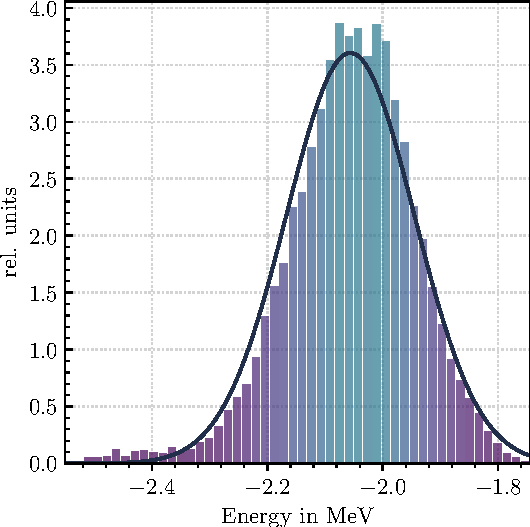
\includegraphics[width=.5\textwidth]{media/example_histogram.pdf}
  \caption{An example histogram of evaluations for a semilocal momentum space regulated chiral interaction of order $N^{2}LO$ with two-body interactions and a cutoff at \SI{450}{\mega\electronvolt} for \n{2}{H} using a SRG flow parmeter of \srg{0.04}. The bar heights have been normed such that the total area of them is 1. The networks are evaluated using sequences from $N_\mathrm{max}=6$ to $N_\mathrm{max}=12$}.
  \label{fig:example_histogram}
\end{wrapfigure}
To evaluate the network, we use a fixed evaluation set consisting of interactions for the three nuclei \n{2}{H}, \n{3}{H} and \n{4}{He}, which were also used in the training as well as the nucleus \n{6}{Li}, to test the extrapolation on a nucleus which was previously unseen by the network. For evaluation, we use semilocal momentum space regulated chiral interactions. Furthermore, each interaction will get evaluated using an SRG evolved hamiltonian with flow parameters of $\alpha = \SI{0.04}{\femto\metre^4}$ and $\alpha = \SI{0.08}{\femto\metre^4}$, to analyze the extrapolations in dependence on the flow parameter. These interactions belong to a different family than the interactions used in training. This means that the network still has to perform an extrapolation, even for the reused nuclei \n{2}{H}, \n{3}{H} and \n{4}{He}.


In the previous section we described the training process of a single network. Since one network can only output one prediction for a given input sequence, we cannot generate a big enough evaluation statistic if we only evaluate the data with one network. To fix that, we train multiple networks which will be evaluated. For our work, 100 networks will be trained to generate a broad statistic.


Since the networks should be applied to heavier nuclei, for which NCSM calculations cannot be done for sufficiently large $N_\mathrm{max}$, we want to analyze how the evaluation changes if we restrict the evaluation samples to certain $N_\mathrm{max}$ values. To demonstrate this evaluation process, we will be using the example of a semilocal momentum space regulated chiral interaction of order N$^{2}$LO with two-body interactions and a cutoff at \SI{450}{\mega\electronvolt} for \n{2}{H} with a SRG flow paramter of \srg{0.04}, for which NCSM calculations have been done with 7 frequencies from $\hbar\Omega = \SI{16}{\mega\electronvolt}$ to $\hbar\Omega = \SI{40}{\mega\electronvolt}$. To simulate a real use case of extrapolation, the evaluation process is first restricted to sequences with $N_\mathrm{max}$ values of 6, 8, 10, 12. Since there are more than 3 frequencies available, a similar inflation process, as described in the previous section, will format the sequences according to the network structure. Now, every single sample can be evaluated by every of the 100 trained networks to generate a broad histogram of predictions. A sample histogram can be seen in \autoref{fig:example_histogram}.


To quantify the evaluation of the networks, we can calculate the mean evaluation as the extrapolated ground state energy as well as the standard deviation to express the error of the extrapolation. To see how the evaluation changes if we consider sequences of higher $N_\mathrm{max}$, we also do this evaluation process for sequences with maximum $N_\mathrm{max}$ of 16, 20 and 24. The data for all those evaluations will be condensed in a single plot for a given nucleus and interaction. In \autoref{fig:example_evaluation}, we see the evaluation of the example interaction from above.

\begin{figure}[H]
  \centering
  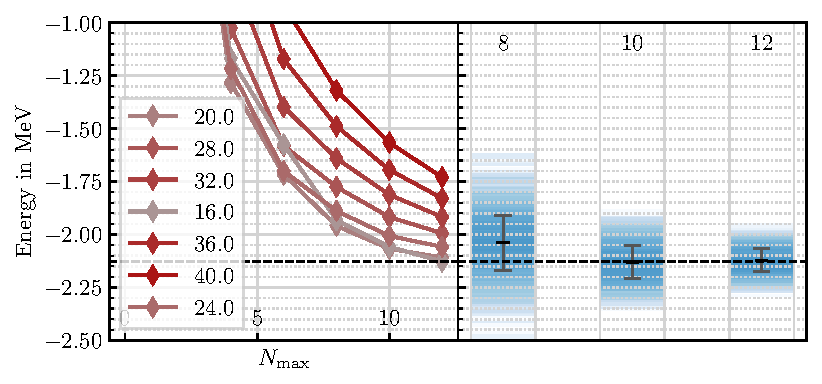
\includegraphics[]{media/example_evaluation.pdf}
  \caption{An example histogram of evaluations for a semilocal momentum space regulated chiral interaction of order $N^{2}LO$ with two-body interactions and a cutoff at \SI{450}{\mega\electronvolt} for \n{2}{H} using a SRG flow parmeter of \srg{0.04}. On the left side the raw NCSM calculations are shown to compare them to the extrapolation. On the right side, for each maximum $N_\mathrm{max}$, the histogramm, as well as its mean and standard deviation is shown, which represent the extrapolated energy and its uncertainty.}
  \label{fig:example_evaluation}
\end{figure}

\section{Classical Extrapolation methods}
To assess our neural network extrapolation method, we want to compare it to classical, state-of-the-art model-space extrapolations. Classical extrapolations are usually done using exponential fits. Even though the convergence of ground state energy sequences does not resemble an exponential convergence, it provides a good estimate on the ground-state energy. To ensure comparability, we resrict the classical extrapolation method to the same $N_\mathrm{max}$ values as in the neural network extrapolation. That means that input sequences are formatted exactly as described earlier, using all subsets of 3 out of all available oscillator frequencies.


In a classical extrapolation, an exponential function
\begin{equation}
  \label{eqn:cl_extr}
  f(x) = a \exp(-bx) + c
\end{equation}
is fitted on a sequence of three $N_\mathrm{max}$ values with a specific oscillator frequency. The resulting limit value $c$ can then be extracted as as the extrapolated value of the ground-state energy. Out of all available frequencies, we choose the frequency which has the lowest energy value at the highest $N_\mathrm{max}$. This is motivated by the fact that these sequences are usually more converged, which ensures more precision in the function fit.

\begin{figure}[H]
  \centering
  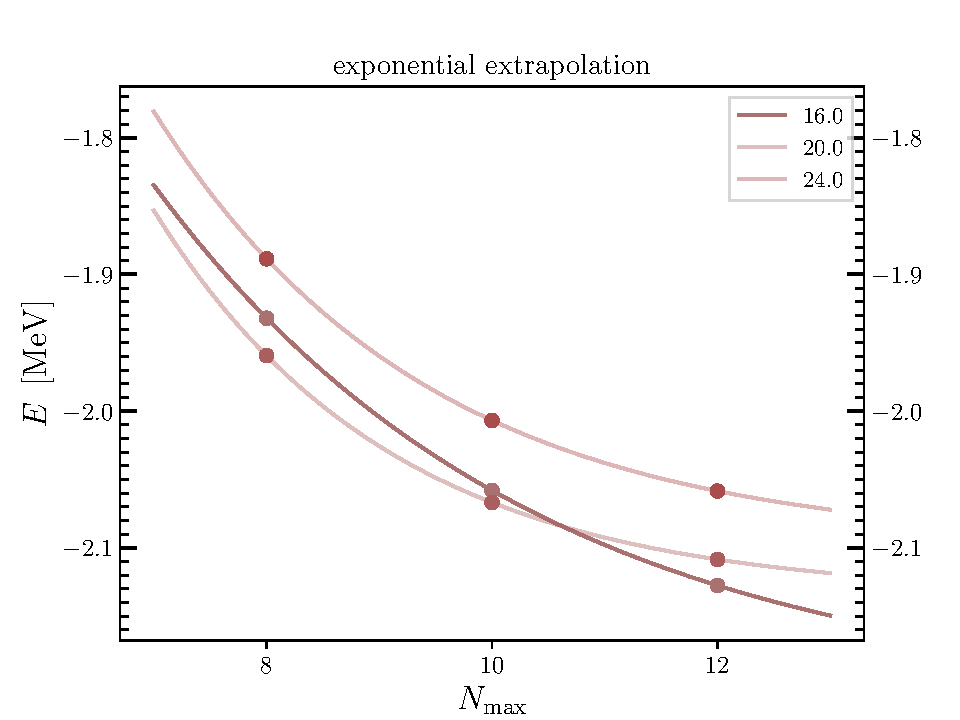
\includegraphics[width=.5\textwidth]{media/example_cl_extr.pdf}
  \caption{For the three different frequencies of $\hbar\Omega = 16, 20, 24$, a function fit of \autoref{eqn:cl_extr} is shown. For the extrapolated ground-state energy, the function fit of the squence with the lowest value for the highest $N_\mathrm{max}$ is chosen. In this example, it is the frequency $\hbar\Omega=16$}
  \label{fig:example_cl_extr}
\end{figure}
For example, if we wanted to extrapolate the sample in \autoref{fig:example_evaluation} with frequencies $\hbar\Omega = 16, 20, 24$ for the case of maximum $N_\mathrm{max}$ of 12, we choose the values  $N_\mathrm{max} = 8, 10, 12$ of the $\hbar\Omega = 16$ sequence for extrapolation, since the absolute value of its sequence is the lowest among the three frequencies at $N_\mathrm{max} = 12$. The resulting function fit is shown in \autoref{fig:example_cl_extr}



\chapter{Extrapolations for the nuclei \n{2}{H}, \n{3}{H} and \n{4}{He}}
\label{chap:reproduction}
In a first application of our extrapolation framework, we want to extrapolate the ground state energies of the nuclei \n{2}{H}, \n{3}{H} and \n{4}{He}, which were already used in the network training and analyze the extrapolation values in dependency on the maximum $N_\mathrm{max}$ of the input sequences. Instead of the many used interactions in the training, we decide on one interaction which will be used as a benchmark to compare this basic extrapolation framework to our more sophisticated methods which will be introduced in the later chapters. We decide on a semi-local momentum space regulated interaction of chiral order 2 with two body interactions and a cutoff at \SI{450}{\mega\electronvolt}. Since this interaction is different to the interactions used in training, we hope to see if the networks captured the characteristics which are own to the nuclei and reproduce those by extrapolating the results of previously unseen interactions.

To investigate the effects of an SRG evolution of the hamiltonian on the extrapolation results, we will further consider the above interaction in the case of an SRG evolution with a paramer of \srg{0.04} and \srg{0.08}.

\section{Results}
In \autoref{fig:eval_vanilla}, the evaluation of the interaction introduced above is shown for the three training nuclei.

% Varbound
An important metric in assessing our extrapolation comes from the variational principles of NCSM calculations for ground-state energies. Since the energies decrease mononously with increasing model-space dimensions, it is guarantied that the exact ground-state energy is lower than all computed NCSM values, regardless of model-space dimension. As a consequence, we can require from a reasonable extrapolation, that the extrapolated energy is lower than the lowest value at the maximum $N_\mathrm{max}$. This mimimum value is called the \textit{variational boundary}. For all maximum $N_\mathrm{max}$ in \autoref{fig:eval_vanilla}, those variational boundaries are shown as dotted lines. We can see that this condition is fulfilled for all nuclei in the case of a flow parameter of \srg{0.04}. Only for the extrapolations of \n{2}{H} with a flow parameter of \srg{0.08}, this condition fails. Additionally, we can also compare the extrapolation result to the variational boundary of highest $N_\mathrm{max}$ available, as this provides a further barrier for which the exact ground-state energy falls under. This barrier is also interesting because it is not indirectly input into the networks, in contrast to the variational boundaries at the maximum $N_\mathrm{max}$, and thus represents a stronger condition for the extrapolation quality of the networks. For the nuclei \n{3}{H} and \n{4}{H}, this condition is also fulfilled. The extrapolations of the energies for the \n{2}{H} nucleus consistently fail to meet this condition.

% Better with higher Nmax
On first sight, the network predictions get more precise if we restrict the evaluation samples to higher values of $N_\mathrm{max}$. This is an indicator that the networks associate steeper slopes of energy sequences with sequences that are not converged already and flat sequences with sequences that are more converged. Based on this, the network tries to extrapolate the steeper sequences with lower predictions and flatter sequences with higher predictions, that lie more closely to the variational boundary. In fact, for the lower values of $N_\mathrm{max}$, the networks generally predict a value for the ground-state energy which is too low in comparison to the variational boundary at the given $N_\mathrm{max}$ or even the variational boundary for the highest available $N_\mathrm{max}$, which is also drawn as a dotted line on the left side of the plots. Furthermore, since the sequences for the different oscillator frequencies converge at different rates, they are further apart for lower $N_\mathrm{max}$ and thus the network extrapolates them on a broader range of energies, resulting in a bigger uncertainties for smaller $N_\mathrm{max}$.
\begin{figure}[H]
  \centering
  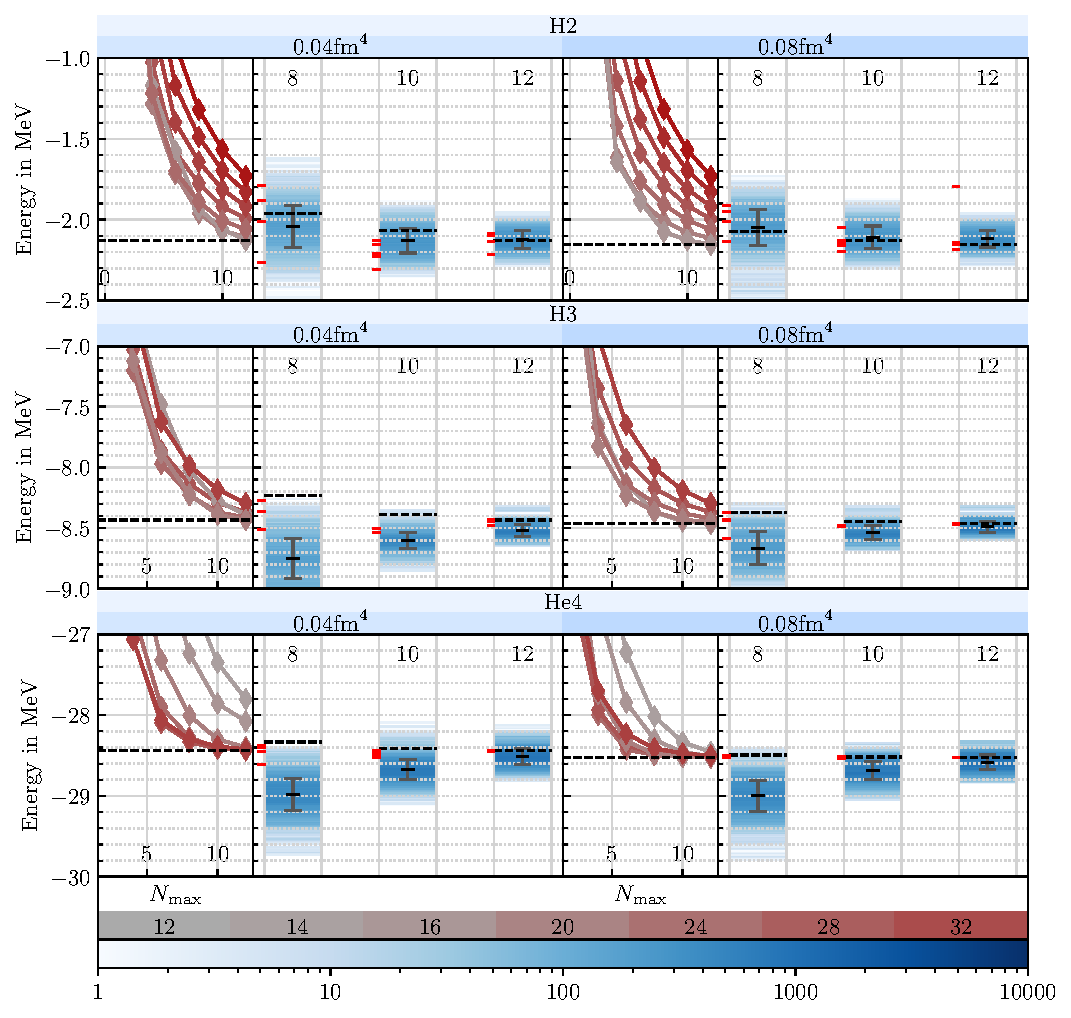
\includegraphics[width=\textwidth]{media/vanilla_evaluation.pdf}
  \caption{Evaluation of our extrapolation method on the nuclei of \n{2}{H}, \n{3}{H} and \n{4}{He}, using a semi-local momentum space regulated interaction of chiral order 2 with two body interactions and a cutoff at \SI{450}{\mega\electronvolt}. For each nucleus and each flow parameter, the NCSM sequences are shown on the left and the extrapolations for a given maximum $N_\mathrm{max}$ on the right. For each maximum $N_\mathrm{max}$, the variational boundary is shown as a dotted line, and the classical extrapolations are shown as red ticks.}
  \label{fig:eval_vanilla}
\end{figure}
% H2 vs rest -> slowest to converge?
An exception to this general extrapolation behaviour of extrapolating too low values for smaller $N_\mathrm{max}$ and correcting the predictions towards the variational boundary for higher $N_\mathrm{max}$ is the nucleus \n{2}{H}. Here, our network shows a systematically different extrapolation behaviour. First, the networks extrapolate the energies not far enough for all $N_\mathrm{max}$. Secondly, the predictions generally get lower if we increase the maximum $N_\mathrm{max}$ of the evaluation samples. This may originate from the fact that the NCSM calculations for \n{2}{H} are the slowest to converge among the three nuclei. The slow convergence results in some sequences having a much flatter slope while still being too high in value with respect to the variational boundary, which is determined by the fastest converging sequence. Another possible origin of this systematic difference is that the training set of nuclei is not balanced evenly between the nuclei and \n{2}{H} may be underrepresented, such that the slow convergence behaviour of \n{2}{H} is foreign to the networks.

% 0.04 vs 0.08
If we look at the differences between the two SRG flow parameters of \srg{0.04} and \srg{0.08}, we see no systematic differences but a general shift of the extrapolations to higher values with respect to their variational boundaries. This is not surprising, since a higher SRG flow parameter leads to faster convergence of the NCSM sequences. This results in lower variational boundaries as well as in a higher extrapolation, which is an effect we already saw in the \n{2}{H} extrapolations.

% Problems: Too low for small nmax

% Comparison classical
% one not converged from H2
% very good for h3, he4 (fast convergence)
% -> only extrapolate "best" frequency
% h2 best example to compare.


\section{Comparison with Classical Extrapolations}
In this section, we want to compare our extrapolation framework to a classical approach of extrapolating NCSM sequences.


\chapter{Influence of training set modifications}
\label{chap:extended}
In the previous chapters, we outlaid a basic extrapolation framework for ground-state energy sequences coming from NCSM calculations. The network extrapolations provided suboptimal results for the fast-to-converge sequences from \n{3}{H} and \n{4}{He}, as the network consistently predicted a too low ground-state energy, especially for the smaller $N_\mathrm{max}$ values, which are important for later use-cases for nuclei whose NCSM calculations cannot be done to a sufficiently high $N_\mathrm{max}$. For the \n{2}{H} nucleus, the networks predicted values which were too high, but comparable to classical extrapolations coming from exponential function fits.

In this section, we want to modify the training step of our extrapolation framework using two different physically motivated \textit{training modes}, to analyze how the training set affects the evaluation of the three nuclei \n{2}{H}, \n{3}{H} and \n{4}{He}. Those modifications only take place in the training of our networks, meaning the evaluation step is unaffected by those modifications such that they can be assessed in the same way as our basic training mode. This also means that our extrapolation framework is still free of any sort of preselection of the evaluation sequences to provide a more general extrapolation, which takes every oscillator frequency into account.
\section{Nmax}
In the training, we deliberately use NCSM calculations which are calculated to a sufficiently high $N_\mathrm{max}$, to extract the limit as a prediction target for the networks. In our basic training mode, the sequences further got divided into subsequences of four consecutive $N_\mathrm{max}$ values. The network then got trained to predict the same limit value for all of those subsequences. Since there are very high $N_\mathrm{max}$ values available, the training set of input sequences also contains sequences with almost constant values, as the sequences have already converged enough to the limit value at that model-space dimension. The result is that the network also gets trained on converged sequences, for which there is no extrapolation needed. In \autoref{fig:example_nmax}, we can see an example sequence which will be used in training. It is clear that sequences above $N_\mathrm{max} \approx 26$ are almost converged and thus provide no new insights for the network about how to extrapolate unconverged sequences. Furthermore, those sequences might even prevent the networks from extrapolating unconverged sequences, as the networks could learn to just reproduce the lowest value of the sequence, as is the case for the converged sequences.

In order to conform to the later use cases of the extrapolation of unconverged sequences, we should also focus our training on the extrapolation of those sequences. To achieve this, we want to restrict the input sequences to lower values of $N_\mathrm{max}$. As we can already see in \autoref{fig:example_nmax}, a restriction of subsequences to a maximum $N_\mathrm{max}$ of 24 will lead to the exclusion of the extreme cases of converged sequences and an inclusion of high enough $N_\mathrm{max}$ values to allow for different convergence rates in the training set.
\begin{figure}[H]
  \centering
  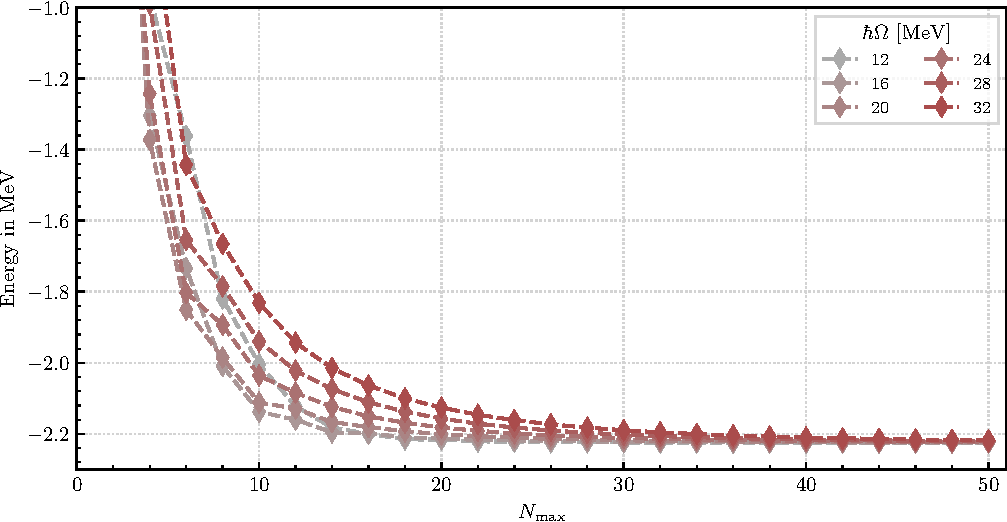
\includegraphics[width=\textwidth]{media/example_sequence.pdf}
  \caption{NCSM results for the $\n{2}{H}$ nucleus. Here, the interaction used for the hamiltonian is \textit{chi2bM3A}. Furthermore, the hamiltionian is SRG evolved using a flow parameter of $\SI{0.04}{\femto\metre^4}$. Each point is the result of a NCSM calculation with a given $N_\mathrm{max}$ and oscillator frequency $\hbar \Omega$.}
  \label{fig:example_nmax}
\end{figure}

\section{srg}
In our second training mode, we want to take another approach to our extrapolation framework as the $N_\mathrm{max}$ limitation training mode. As we have already seen, a SRG evolution of the Hamiltonian results in a faster convergence of the NCSM sequences. Taking this into account, we can also try to train the networks only using NCSM calculations with SRG evolved Hamiltonians using a minimum flow parameter of \srg{0.04}. In doing this, we hope to achieve a more uniform and stronger convergence in the different sequences in the training, such that the networks do not have to extrapolate as much as with unconverged sequences. This will also be useful for the later uses of the extrapolation on heavier nuclei, as an SRG evolution can always be done.

\section{results and comparison}
In order to evaluate the training-modified versions of our extrapolation framework, we have to make sure that the evaluation data conforms to the restrictions that we apply to our training set to ensure consistency. In our first training mode, the used $N_\mathrm{max}$ are restricted to be lower than 24. In the second training mode, only interactions which are SRG evolved using a flow parameter of at least \srg{0.04} are used. Our evaluation set, consisting of $N_\mathrm{max}$ values up to 12 and of interactions evolved using a flow parameter of \srg{0.04} and \srg{0.08}, already satisfies these requirement.
\begin{figure}[H]
  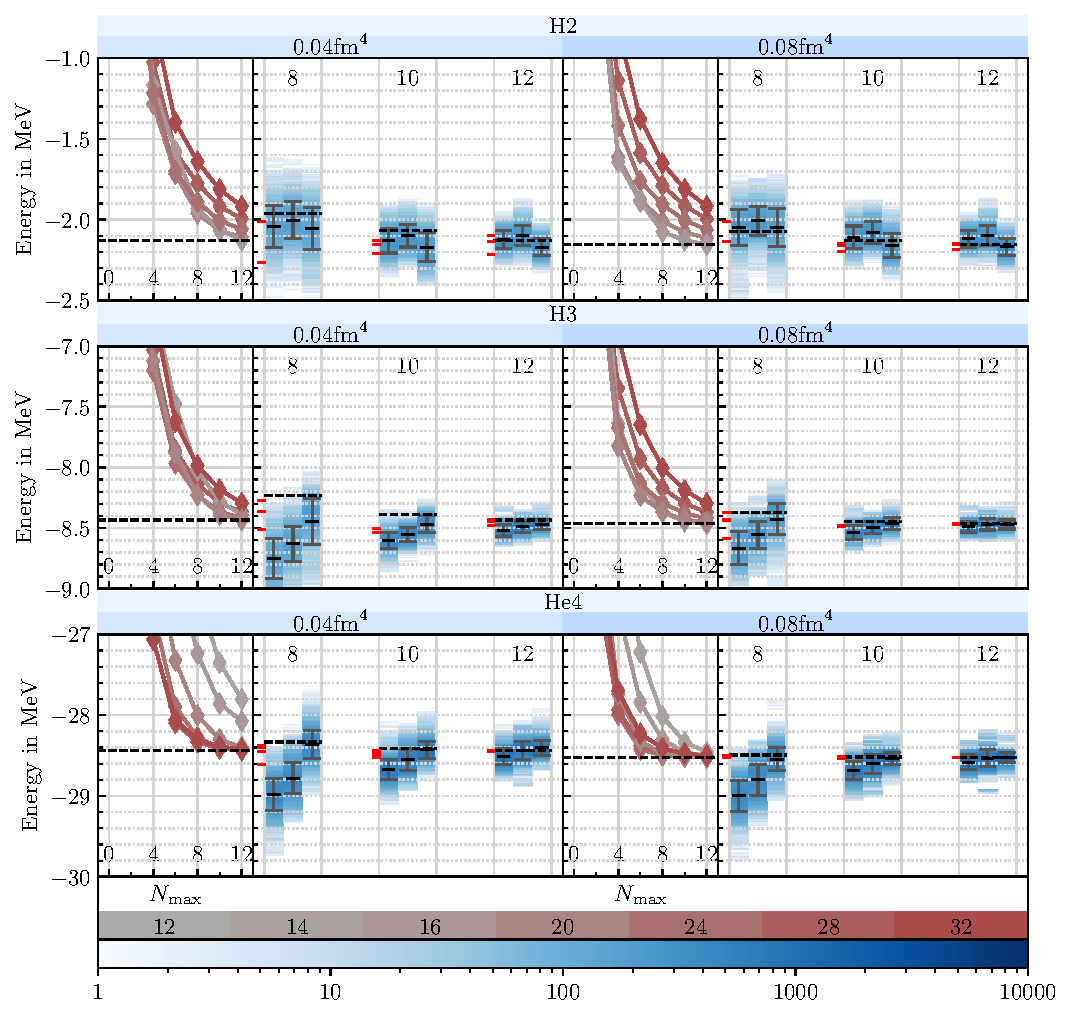
\includegraphics[width=\textwidth]{media/extended_evaluation_ohne_fehlfit.pdf}
  \caption{Evaluation of our training modes on the nuclei \n{2}{H}, \n{3}{H} and \n{4}{He}, using a semi-local momentum space regulated N$^2$LO interaction with two-body interactions and a cutoff at \SI{450}{\mega\electronvolt} \cite{smsquelle}. The shown training modes are, in order from left to right, the basic training mode for comparison, the $N_\mathrm{max}$-limitation training mode and the SRG-filter training mode. For each nucleus and each flow parameter, the NCSM sequences are shown on the left (the different frequencies are colored respectively to the legend, which shows the frequencies $\hbar\Omega$ in \si[]{\mega\electronvolt}) and the extrapolations for a given maximum $N_\mathrm{max}$ on the right. For each maximum $N_\mathrm{max}$, the variational boundary is shown as a dashed line, and the classical extrapolations are shown as red ticks.}
  \label{fig:eval_extended}
\end{figure}

\autoref{fig:eval_extended} displays the evaluation of the three nuclei. Each histogram at every $N_\mathrm{max}$ is now divided into three seperate histograms, showcasing the evaluation result for the different training modes. In each stack of histograms, the leftmost is the basic training mode already introduced in \autoref{chap:framework} and assessed in \autoref{chap:reproduction}. The histogram in the center corresponds to our first training mode, which restricts the $N_\mathrm{max}$ in the training process to at most 24. The rightmost histogram is our second introduced training mode, which restricts the type of training interactions to SRG evolved interactions with a flow parameter of at least \srg{0.04}.

We again begin by looking at the nuclei \n{3}{H} and \n{4}{He}. For both training modes, we see that the predictions get closer to the variational boundary, which means that the training modes yield overall better predictions, since the sequences are already converged enough. Interestingly, the two training modes seem to only impact the accuracy of the prediction. The uncertainty of both training modes are comparable to the uncertainty of the prediction by the basic extrapolation framework.

If we compare the two training modes for those nuclei, we see that the $N_\mathrm{max}$-limitation mode is less impactful than the SRG-filter mode. This can be explained by the fact that the some of the sequences of the \n{3}{H} and the \n{4}{He} nucleus are already converged enough. Since we explicitly remove bare Hamiltonians in the SRG-filter mode, the training set gets limited to a smaller size of fast converging sequences, thus training the net better to those cases. This can especially be seen in the \n{4}{He} nucleus, where there are sequences which have a very strong convergence rate. Here, the SRG-filter mode results lie very close to the variational boundary. The limitation on the $N_\mathrm{max}$ values also have a positive impact on the evaluation. This may indicate that the networks have learned from the constant sequences of high $N_\mathrm{max}$ values to linearly extrapolate the results up to a certain point, which results in the predictions being unreasonably low for low $N_\mathrm{max}$ sequences, as is the case for our basic extrapolation framework.
% 3h, 4he:
% nmax: a bit better
% srg: way better

For the nucleus \n{2}{H}, our basic framework showed a totally different systematic behavior than for the nuclei \n{3}{H} and \n{4}{He}. This is also the case for both new training modes. Especially the $N_\mathrm{max}$ training mode seems to extrapolate not far enough, such that the predictions do not conform to the variational boundary at $N_\mathrm{max} = 12$. Even though the $N_\mathrm{max}$-limitation mode is thought to handle unconverged sequences better than the unmodified training mode, it predicts higher ground-state energies for both SRG flow parameters and for all $N_\mathrm{max}$ values. This can be explained by the fact that the \n{2}{H} sequences are not only converged until $N_\mathrm{max} = 12$, but also converge quite slowly. This leads to a very broad range of energy values at $N_\mathrm{max} = 12$ for all the frequencies, but the sequences themself are relatively flat, leading to a higher prediction of the $N_\mathrm{max}$-limitation training mode. The SRG-filter training mode seems to perform better than the basic training mode. Even though this training mode still produces unreasonably high predictions for $N_\mathrm{max} = 8$, the predictions for all $N_\mathrm{max} \geq 10$ are lower than the variational boundary at $N_\mathrm{max} = 12$. This is a great improvement over the other two training modes.

The comparison between the two different SRG flow parameters yield the same results as in the previous chapter, where we have considered our training without further modifications. We can see that the network predictions do not change much when evaluating the higher srg flow parameter. This is especially interesting in the case of \n{4}{He}, where the difference between the NCSM sequences is the biggest. At $\alpha = \srg{0.04}$, the lower sequences of $\hbar \Omega = \SI{12}{\mega\electronvolt}$ and \SI{14}{\mega\electronvolt} are converging fast, but they have not reached a sufficient degree of convergence, such that the values at $N_\mathrm{max} = 12$ are still spread far apart. For $\alpha = \srg{0.08}$, those sequences have converged sufficiently until $N_\mathrm{max} = 12$. We can see that the networks react very consistently between the different sequences.
% 2h:
% nmax worse than vanilla (WHY?)
% nmax geq 10: srg under varbound!

% difference srg
% same as vanilla: extrapolations go up



\section{conclusion}
In this chapter, we have extended our basic extrapolation framework by modifying the training process of the neural networks in two distinct ways to see how they affect the extrapolation of ground-state energies. In a first modification, we have decided on only training the networks by using sequences up to $N_\mathrm{max} = 24$. In a second modification, the networks were only trained by NCSM sequences coming from SRG evolved Hamiltionians with a flow parameter $\alpha$ of \srg{0.04} or higher. We have discussed these \textit{training modes} by evaluating the nuclei \n{2}{H}, \n{3}{H} and \n{4}{He} and comparing the results to our basic training mode from \autoref{chap:reproduction}.

To classify our training modes, we first provide two important aspects that those training modes have to show. Firstly, they should result in extrapolations which are "better" in some way when compared to the unmodified training process. For example, they should either result in a smaller uncertainty or in a different prediction which is more reasonable given the NCSM sequences. Secondly, a modification of the training set should result in consistent extrapolations across different scenarios, such as unconverged NCSM sequences and NCSM sequences with a low convergence rate.

Keeping these conditions in mind, we conclude that the SRG-filter training mode so far provided the most reasonable results across all nuclei. The unmodified training mode, as well as the $N_\mathrm{max}$-limitation training mode, predicted unreasonably low ground-state energies for the nuclei \n{3}{H} and \n{4}{He} yet unreasonably high energies for \n{2}{H}. For all of these nuclei, the SRG-filter training mode provided more reasonable predictions. Also, the SRG-filter training mode provided the most consistent results, since it can handle the more converged and more unconverged sequences of \n{3}{H} and \n{4}{He} respectively, as well as the slow converging sequences of \n{2}{H}.

The $N_\mathrm{max}$-limitation filter provided more reasonable results for \n{3}{H} and \n{4}{He}, but too high values for \n{2}{H}, even higher than the unmodified training mode, making it the most unconsistent and unreasonable among the two training modes discussed.

Considering all of the above, it seems that the SRG-filter training mode provides the most promising results. In order to reach a final verdict about the two training modes, we will test how they behave in a scenario which is closer to a real use-case of an extrapolation in \autoref{chap:li6}, where we evaluate the NCSM calculations for the nucleus \n{6}{Li}.
% CONCLUSION
% srg can handle converged and unconverged sequences can be seen by h2 and he4
% Nmax cant handle slow converging sequences



\chapter{Difference based extrapolation framework}
\label{chap:diff}
\IMRADlabel{discussion}
In our basic extrapolation framework, we trained networks on predicting the exact ground-state energy given a few sequences of absoulte energy values. This method is inherently dependent on the absolute values of the energy, since the networks fundamentally consist of linear maps from one layer to the next. Nuclear ground-state energies have a very broad range, which we already saw in our inspected nuclei. For example, \n{2}{H} has a ground-state energy of approximately \SI{-2.1}{\mega\electronvolt} and \n{4}{He} has a ground-state energy of approximately \SI{-28.4}{\mega\electronvolt}, based off the NCSM calculations shown in \autoref{fig:example_nmax} and \autoref{fig:eval_extended}. As a result, we cannot confidentially exclude the possibility of the absolute ground-state energies influencing the network predictions.

In this chapter, we want to analyze the influence of the absolute energies on the network prediction by implementing a different extrapolation method based on our previous framework, which will work by extrapolating the differences of the energy sequences.
\section{framework}
In order to implement our difference based extrapolation framework, we have to think about how we have to change the generation of the input data, the network structure as well as the extrapolation process of our basic extrapolation framework.

We want to base our network training on the same data set as the basic framework. The networks now should get the differences of consecutive ground-state energies in the sequences as an input. To achieve this, we generate the same formatted input sequences out of the raw NCSM calculations, using the inflation algorithm described in \autoref{sec:inflate}. The formatted input data thus consists of four consecutive energy values for three oscillator frequencies, as well as a limit which will be used to compute the prediction target of our networks. To turn those sequences into our input difference sequences, we calculate the three differences between the four energy values. When the networks get input data in the form of energy differences, they cannot possibly predict an absolute ground-state energy from them. This means that the prediction target will also have to be modified to a difference. It is natural to take the difference between the last value of the energy sequence and the limit as a target. However, this leads to a problem, as the limit is the same for the three oscillator frequencies for a given nucleus and interaction, but the last values of the energy sequences can vary depending on the frequency. Because the three difference sequences are all put into a network simultaneously, we have to find a single common extrapolation target. For this, we decide to take the difference between the mean of the last values for all three sequences and the limit.

Note that, since we now only have three direct inputs available, which consist of the differences of the four absolute values, the network structure has to be adjusted to be compatible with this data. For the input layer, we have $L^{(1)} = 3 \times 3 = 9$ input neurons. Furthermore, we reduce some of the hidden neurons in the hidden layers to accommodate the reduced input neurons. We empirically decide on $L^{(2)} = 18$, $L^{(3)} = 12$. The single output neuron stays the same. We could have chosen to keep the network structure the same, but this would require to input four differences of five energies, which would mean that those networks got more information about the sequences. To ensure comparability, we chose to keep the information the same but adjust the network structure.

Further modifications include the adjustment of our sequence shifting. In our basic framework, we decided to shift the formatted sequences by a random amount of $[\SI{-10}{\mega\electronvolt}, \SI{10}{\mega\electronvolt}]$ to counter the dependency on absolute values. They are no longer needed, as they would cancel out when calculating the differences. Also, the threshold for deeming a network valid is reduced to \SI{0.1}{\mega\electronvolt}, as the energy differences which are input are generally much smaller than the absolute values.

To compensate for the shift in the training set, we also have to modify the evaluation of a network. The evaluation will work the same way as in our basic framework, but now, the final prediction is calculated by adding the mean of the last energy values back onto the network prediction.

\section{results and comparison}
Using our newly constructed difference-based extrapolation framework, we can now do the same analysis on our three nuclei \n{2}{H}, \n{3}{H} and \n{4}{He} using the same interaction as used earlier. Even though the difference-based framework computes a difference prediction internally, the final evaluation will still base off the same absolute energy differences and result in an absolute energy prediction. This means that we can apply our different evaluation modifications from \autoref{chap:extended} and discuss the influences of them on the difference based evaluation. Furthermore, using the same nuclei allows us to compare the difference based extrapolation and the absolute value extrapolation.

The results of our difference based extrapolation is shown in \autoref{fig:eval_diff}. The final extrapolated values and their uncertainty are shown in \autoref{tab:eval_diff} as well for each $N_\mathrm{max}$ and each SRG flow parameter.

% Generell: Predictions VIEL genauer, besonders bei hohem Nmax
Looking at all three nuclei, we can see that the uncertainty of all training modes is drastically reduced. Especially for higher $N_\mathrm{max}$, the predictions get very precise. Furthermore, the absolute value of the predictions are generally way closer to a reasonable limit. This can be seen for the nuclei \n{4}{He} and \n{3}{H}, where the networks trained with the unmodified or the $N_\mathrm{max}$-limitation training mode in the absolute based extrapolation framework predicted unreasonably low values for all $N_\mathrm{max}$. This could be caused by the fact that the absolute values are purged from the resulting differences, such that the absolute value of the sequences do not matter in the extrapolation process. This leads to a focus on the convergence of the sequences. When the sequence converges, the differences tend towards zero, such that evaluation yields a prediction for the ground-state energy close to the last values in the inputted sequences. There is a disadvantage of the difference-based extrapolation in the nucleus \n{4}{He} for a flow parameter of $\alpha = \srg{0.04}$. Here, the sequences converge fast, but for the small values of $N_\mathrm{max}$ given, the sequences are cut off for the lower oscillator frequencies of $\hbar\Omega = \SI{12}{\mega\electronvolt}$ and \SI{14}{\mega\electronvolt}. This leads to the network recieving a broad range of differences, resulting in a greater uncertainty for the ground-state energy prediction. We can also see that this effect gets better for $\alpha = \srg{0.08}$, where even the sequences for the lower oscillator frequencies are now visibly more converged to the limit.

% H2: 0.08 schlechter als 0.04

\begin{table}[H]
  \caption{Extrapolation results in \si[]{\mega\electronvolt} of the difference based framework for the nuclei \n{2}{H} \textbf{(a)}, \n{3}{H} \textbf{(b)} and \n{4}{He} \textbf{(c)}. For each interaction characterized by the flow parameter $\eta = \srg{0.04}, \srg{0.08}$, the final extrapolation results for the given $N_\mathrm{max}$ value is shown. Here, \textbf{(1)} is our basic extrapolation without further modifications of the training step, \textbf{(2)} is the $N_\mathrm{max}$-limitation training mode, \textbf{(3)} is the SRG-filter training mode. }
  \label{tab:eval_diff}
  \centering
  \begin{subtable}{\textwidth}
    \caption{}
    \centering
    \begin{tabular}{
        r|
        S[table-format=-2.3(3)]
        S[table-format=-2.3(3)]
        S[table-format=-2.3(3)]
        S[table-format=-2.3(3)]
        S[table-format=-2.3(3)]
        S[table-format=-2.3(3)]
      }
      \toprule
      $\eta$                           &
      \multicolumn{3}{c}{$\srg{0.04}$} &
      \multicolumn{3}{c}{$\srg{0.08}$}   \\
      \midrule
      $N_\mathrm{max}$                 &
      {8}                              &
      {10}                             &
      {12}                             &
      {8}                              &
      {10}                             &
      {12}                               \\
      \midrule
      (1)                              &
      -2.066 \pm 0.065                 &
      -2.144 \pm 0.025                 &
      -2.129 \pm 0.022                 &
      -2.054 \pm 0.069                 &
      -2.113 \pm 0.028                 &
      -2.126 \pm 0.023                   \\
      (2)                              &
      -2.080 \pm 0.055                 &
      -2.146 \pm 0.023                 &
      -2.127 \pm 0.020                 &
      -2.064 \pm 0.056                 &
      -2.110 \pm 0.026                 &
      -2.124 \pm 0.022                   \\
      (3)                              &
      -2.068 \pm 0.055                 &
      -2.153 \pm 0.038                 &
      -2.149 \pm 0.034                 &
      -2.062 \pm 0.041                 &
      -2.124 \pm 0.032                 &
      -2.158 \pm 0.036                   \\
      \bottomrule
    \end{tabular}
  \end{subtable}
  \par\bigskip
  \begin{subtable}{\textwidth}
    \caption{}
    \centering
    \begin{tabular}{
        r|
        S[table-format=-2.3(3)]
        S[table-format=-2.3(3)]
        S[table-format=-2.3(3)]
        S[table-format=-2.3(3)]
        S[table-format=-2.3(3)]
        S[table-format=-2.3(3)]
      }
      \toprule
      $\eta$                           &
      \multicolumn{3}{c}{$\srg{0.04}$} &
      \multicolumn{3}{c}{$\srg{0.08}$}   \\
      \midrule
      $N_\mathrm{max}$                 &
      {8}                              &
      {10}                             &
      {12}                             &
      {8}                              &
      {10}                             &
      {12}                               \\
      \midrule
      (1)                              &
      -8.453 \pm 0.099                 &
      -8.528 \pm 0.044                 &
      -8.470 \pm 0.026                 &
      -8.410 \pm 0.090                 &
      -8.465 \pm 0.035                 &
      -8.460 \pm 0.025                   \\
      (2)                              &
      -8.461 \pm 0.082                 &
      -8.526 \pm 0.036                 &
      -8.468 \pm 0.025                 &
      -8.422 \pm 0.074                 &
      -8.464 \pm 0.031                 &
      -8.457 \pm 0.023                   \\
      (3)                              &
      -8.390 \pm 0.064                 &
      -8.493 \pm 0.028                 &
      -8.466 \pm 0.026                 &
      -8.408 \pm 0.045                 &
      -8.460 \pm 0.026                 &
      -8.466 \pm 0.025                   \\
      \bottomrule
    \end{tabular}
  \end{subtable}
  \par\bigskip
  \begin{subtable}{\textwidth}
    \caption{}
    \centering
    \begin{tabular}{
        r|
        S[table-format=-2.3(3)]
        S[table-format=-2.3(3)]
        S[table-format=-2.3(3)]
        S[table-format=-2.3(3)]
        S[table-format=-2.3(3)]
        S[table-format=-2.3(3)]
      }
      \toprule
      $\eta$                           &
      \multicolumn{3}{c}{$\srg{0.04}$} &
      \multicolumn{3}{c}{$\srg{0.08}$}   \\
      \midrule
      $N_\mathrm{max}$                 &
      {8}                              &
      {10}                             &
      {12}                             &
      {8}                              &
      {10}                             &
      {12}                               \\
      \midrule
      (1)                              &
      -28.502 \pm 0.397                &
      -28.497 \pm 0.212                &
      -28.405 \pm 0.095                &
      -28.520 \pm 0.175                &
      -28.535 \pm 0.064                &
      -28.529 \pm 0.025                  \\
      (2)                              &
      -28.399 \pm 0.319                &
      -28.454 \pm 0.177                &
      -28.391 \pm 0.080                &
      -28.522 \pm 0.143                &
      -28.537 \pm 0.052                &
      -28.530 \pm 0.021                  \\
      (3)                              &
      -28.377 \pm 0.294                &
      -28.408 \pm 0.139                &
      -28.353 \pm 0.054                &
      -28.507 \pm 0.065                &
      -28.521 \pm 0.026                &
      -28.527 \pm 0.012                  \\
      \bottomrule
    \end{tabular}
  \end{subtable}
\end{table}


Another effect of the difference based extrapolation is that the different training modes now generally predict a ground-state energy in the same range. However, now the impact of the training modes has shifted from the absolute value of the prediction into the uncertainty of the prediction. This can be seen especially for the SRG-filter training mode, where the uncertainty generally gets smaller for the nuclei \n{3}{H} and \n{4}{He}, but larger for \n{2}{H}, which can be attributed to the slow convergence of \n{2}{H} sequences.
For the first and second training mode of the \n{2}{H} nucleus, we can also observe that the difference based framework produces a smaller uncertainty than the range of the classical extrapolations.

For \n{2}{H} and \n{3}{H}, we can also see that the predictions for the ground-state energy are a bit higher for the SRG flow parameter of \srg{0.08} than \srg{0.04}.

Note that the difference based extrapolation framework is not completely independent of the absolute values of the sequences, since the prediction target for the network training is calculated using the average of the absolute values for the highest $N_\mathrm{max}$. This can also result in a dependency on the spread of the different sequences for the evaluated maximum $N_\mathrm{max}$.

\begin{figure}[H]
  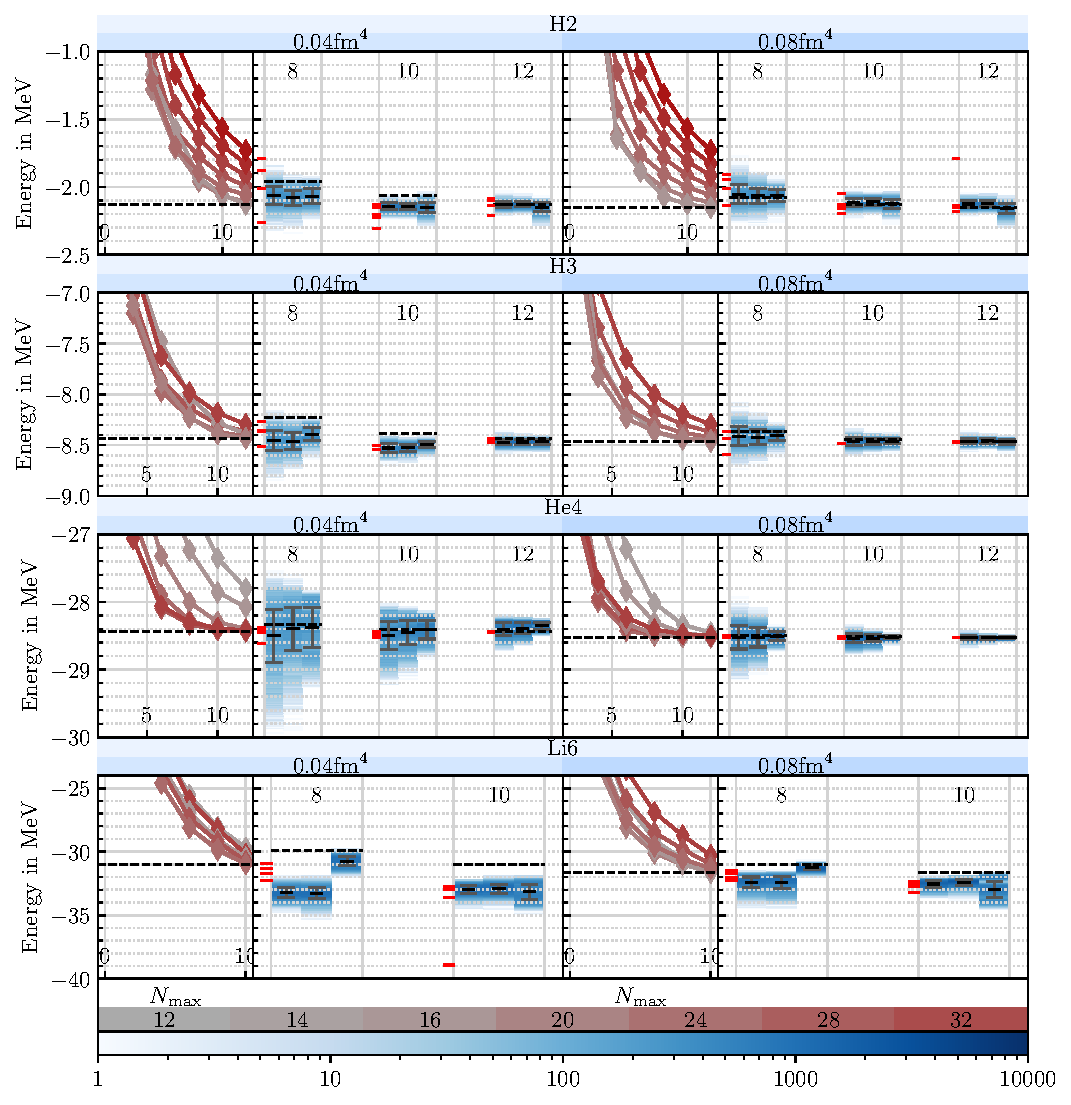
\includegraphics[width=\textwidth]{media/diff_evaluation.pdf}
  \caption{Evaluation of our training modes on the nuclei \n{2}{H}, \n{3}{H} and \n{4}{He} in the difference based extrapolation framework. The shown training modes are, in order from left to right, the basic training mode for comparison, the $N_\mathrm{max}$-limitation training mode and the SRG-filter training mode. For each nucleus and each flow parameter, the NCSM sequences are shown on the left (the different frequencies are colored respectively to the legend, which shows the frequencies $\hbar\Omega$ in \si[]{\mega\electronvolt}) and the extrapolations for a given maximum $N_\mathrm{max}$ on the right. For each maximum $N_\mathrm{max}$, the variational boundary is shown as a dashed line, and the classical extrapolations are shown as red ticks.}
  \label{fig:eval_diff}
\end{figure}


\section{conclusion}


\chapter{Extrapolation of \n{6}{Li}}
\label{chap:li6}
\IMRADlabel{results}
In a final application of both the absolute and the difference based extrapolation frameworks, we want to evaluate the nucleus \n{6}{Li} by using the same interaction as in the previous chapters.

This application will be special because \n{6}{Li} is not present in the training set. Furthermore, \n{6}{Li} has a higher mass than all of the nuclei considered before. As a result, we can regard \n{6}{Li} as a nucleus for which NCSM calculations can not be done until a sufficiently high $N_\mathrm{max}$, such that extrapolation of the ground-state energy is needed. The evaluation of the \n{6}{Li} extrapolation can thus be considered as a first test of our extrapolation frameworks in a real use-case scenario.
\section{Results}
\begin{figure}[H]
  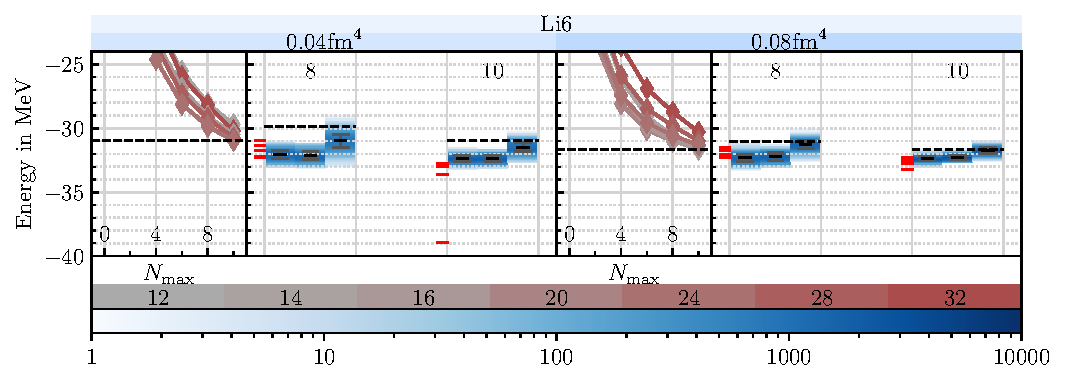
\includegraphics[width=\textwidth]{media/li6_evaluation_abs.pdf}
\end{figure}

\begin{figure}[H]
  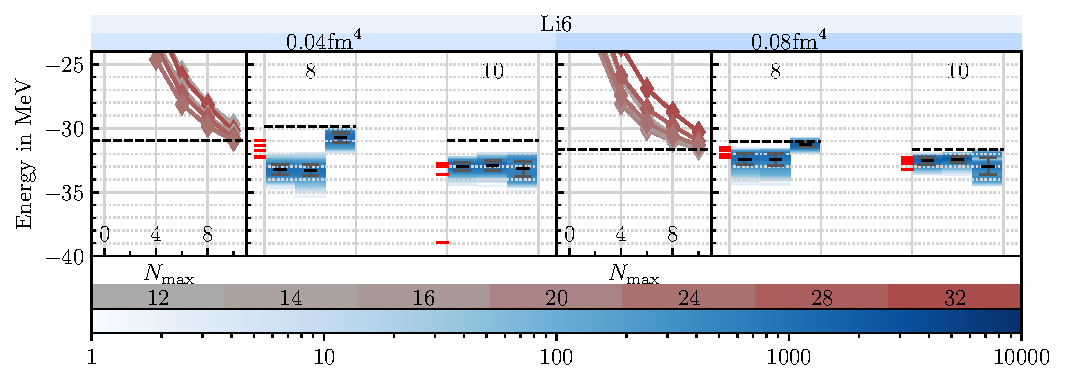
\includegraphics[width=\textwidth]{media/li6_evaluation_diff.pdf}
\end{figure}

\section{Conclusion}
In this chapter, we have applied both of the previously presented absolute and difference based extrapolation frameworks to the nucleus \n{6}{Li}. For that, we have simulated a real use-case scenario by using NCSM calculations up to $N_\mathrm{max} = 10$.

Using the observations obtained from the \n{6}{Li}, we can decide on a final choice for the training mode and framework, which will be used to produce a final prediction for the \n{6}{Li} nucleus.

Now that we have applied the different training modes and the two framework to a real use-case, we are ready to formulate our final verdict about the frameworks as well as the training modes. For the training modes, we have already formulated two conditions that are necessary. They have to provide more reasonable predictions than the unmodified training mode and be consistent. In the previous chapters, we have seen that the $N_\mathrm{max}$-limitation training mode yielded inconsistent predictions for three training nuclei. This conforms to our observations in the evaluation of \n{6}{Li}, where the training mode produced reasonable but inconsistent results. The SRG-filter training mode was deemed the most promisable one in the evaluation of the three training nuclei. Unfortunately, this training mode resulted in the predictions of very unreasonably high values for the \n{6}{Li} nucleus.

Each of the training modes provided good results in some cases, but worse results than the unmodified training in other cases. Based on this inconsistency, we decide that the unmodified training mode is the most stable across all different scenarios, which is why we will be using this mode in our final result for \n{6}{Li}.

Now we come to a verdict about the two different extrapolation frameworks. The first framework consisted of the extrapolation of sequences of absolute energy values, while the second framework consisted of extrapolating difference sequences. While we observed that the difference based framework produced a little smaller uncertainty for \n{6}{Li}, we saw in the previous chapters \ref{chap:extended} and \ref{chap:diff}, that the difference based framework produced more reasonable predictions and generally smaller uncertainties as the absolute based framework. For that reason, we decide on the difference based framework as the generally better method of extrapolating ground-state energies.

Using the difference based framework as well as the unmodified training process, we can state a final extrapolation result for the \n{6}{Li} nucleus. Since we have two maximum $N_\mathrm{max}$ values available, we have to decide on one for the final extrapolation. In a real use-case, one would decide on the maximum $N_\mathrm{max}$ available in order to input the maximum amount of information about the sequence limit into the network, as the higher $N_\mathrm{max}$ values are more converged. Using this, we decide on the extrapolation result of $N_\mathrm{max} = 10$ as the final prediction of the \n{6}{Li} ground-state energy value, which is given by \SI{-32.976 \pm 0.329}{\mega\electronvolt} for the interaction evolved with a flow parameter of \srg{0.04} and \SI{-32.542 \pm 0.272}{\mega\electronvolt} for the flow parameter of \srg{0.08}. The histograms of those extrapolations can be found in \autoref{fig:hists_li6}.

For the computation of the final prediction, as well as the error estimate, we assumed that the network prediction are normally distributed. The distribution of the predictions for the flow paramter $\alpha$ of \srg{0.04} shows a good compliance to the shown normal distribution. However, we also see that the distribution is slightly skewed towards lower energy values. This effect is amplified in the distribution of predictions for $\alpha = \srg{0.08}$, where there is a sharp decline in predictions for high energies bigger than \SI{-32.1}{\mega\electronvolt}, but a higher amount of predictions for lower energies. As a result, the assumption of a normal distribution leads to a lower prediction than the most guessed value. To generate a more meaningful prediction and uncertainty, we could assume a probability density that takes this skewness into account.

\begin{figure}[H]
  \begin{subfigure}{.5\textwidth}
    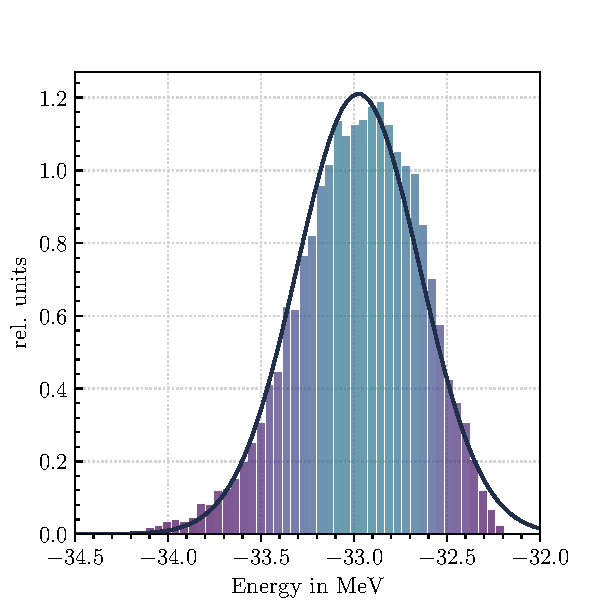
\includegraphics[width=\textwidth]{media/li6_0400_histogram.pdf}
    \caption{}
  \end{subfigure}
  \begin{subfigure}{.5\textwidth}
    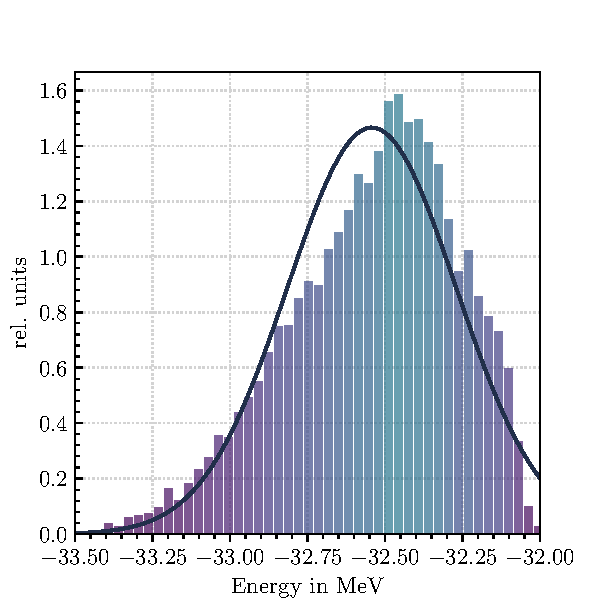
\includegraphics[width=\textwidth]{media/li6_0800_histogram.pdf}
    \caption{}
  \end{subfigure}
  \caption{Histograms for the final extrapolation of \n{6}{LI} for the different SRG flow parameters of \srg{0.04} \textbf{(a)} and \srg{0.08} \textbf{(b)}. The bar heights have been normed such that the total area of them is 1. The final extrapolation used the difference based framework together with an unmodified training process.}
  \label{fig:hists_li6}
\end{figure}



\chapter{Outlook}
\label{chap:outlook}

In this final chapter, we want to look at a few ideas that are based on our extrapolation framework that could further improve the extrapolation of ground-state energies using neural networks.

In a first idea, we want to look at another training modification which will work by dynamically filtering frequencies.

In a second idea, we demonstrate the effect of preselecting frequencies on the extrapolation.

Last, we want to outlay three different general approaches to the idea of using neural networks as an extrapolation tool for ground-state energies.
\section{Frequency filter}
\begin{wrapfigure}{r}{.5\textwidth}
  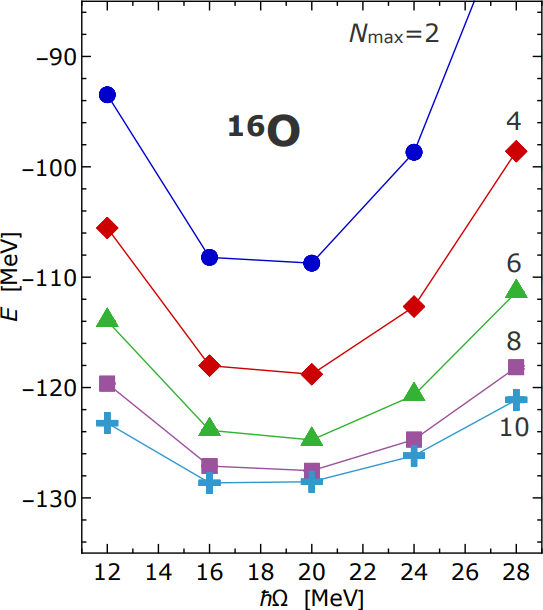
\includegraphics[width=.5\textwidth]{media/freq_filter.png}
  \caption{NCSM calculations for \n{16}{O} in dependency on the used oscillator frequency \cite{sommerschule}.}
  \label{fig:freq_dependency}
\end{wrapfigure}
The single-particle harmonic oscillator basis is not asymptotically good to approximate the states of nuclei, as harmonic oscillator wave functions fall off like a gaussian function, but bound states in a potential well typically fall off like an exponential function \cite{sommerschule}. Furthermore, the composition into the harmonic oscillator Slater determinants is dependant on a free parameter for the oscillator frequency. This oscillator frequency also defines the oscillator length and thus the spatial resolution for the basis states.

As we have already seen, the dependence on the oscillator frequency results in different convergence rates for our NCSM sequences. In fact, NCSM calculations using harmonic oscillator Slater determinants typically show a parabolic convergence behaviour with respect to the used oscillator frequency. This is shown in \autoref{fig:freq_dependency} for the nucleus \n{16}{O}. As a consequence, there is a special frequency, for which an optimal convergence rate is to be expected. In \autoref{fig:freq_dependency}, this minimum frequency is given by $\hbar \Omega = \SI{20}{\mega\electronvolt}$.

In order to capture those different convergence rates, we want to restrict the sequences used to either side of the minimum, resulting in two training modes. In the first training mode, only sequences smaller than the frequency minimum are used, such that the network will get more information of the long range behaviour of the nucleonic interaction. As a result, the networks have to model the short range behaviour. Conversely, in the second training mode, the networks will be trained on the short range behaviour by restricting the frequencies to the ones higher than the minimum, thus modeling long range behaviour.

To implement this, we dynamically compute the frequency, for which the lowest value is achieved at $N_\mathrm{max} = 8$ for each NCSM calculation. This frequency will be used to filter the frequencies for the training. In both cases, we include the frequency minimum, as that is the frequency with the best convergence behaviour.



\begin{figure}[H]
  \begin{subfigure}{\textwidth}
    \centering
    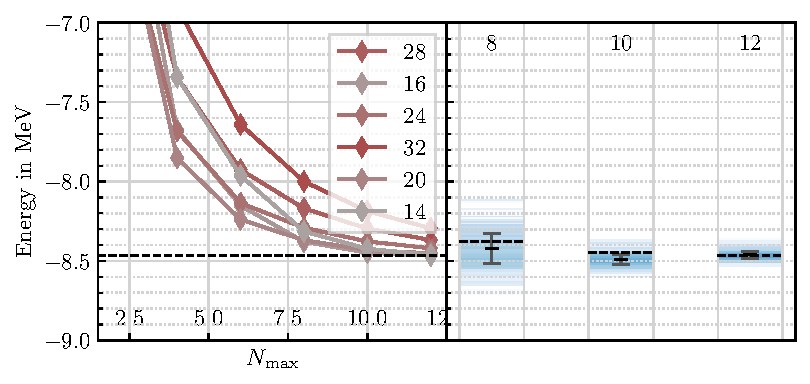
\includegraphics{media/outlook_frequency_lower.pdf}
    \caption{}
  \end{subfigure}
  \begin{subfigure}{\textwidth}
    \centering
    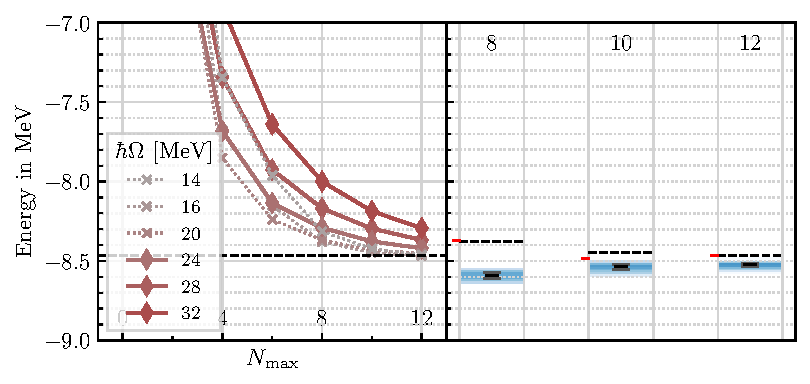
\includegraphics{media/outlook_frequency_higher.pdf}
    \caption{}
  \end{subfigure}
  \caption{Evaluation of the frequency filter training mode on \n{3}{H} with the interaction specified above. The frequencies used in the evaluation are shown with solid lines. To achieve a better comparability with the previous extrapolations, the frequencies not taken into account are shown as dotted lines. In \textbf{(a)}, the networks were trained on the low frequencies, thus modeling the short range behaviour. In \textbf{(b)}, the networks were trained on the high frequencies, thus modeling the long range behaviour.}
  \label{fig:eval_freqfilter}
\end{figure}

We look at a single example of the \n{3}{H} nucleus, using a semi-local momentum space regulated N$^{4}$LO interaction with two-body interactions and a cutoff at \SI{450}{\mega\electronvolt} alongside a SRG evolution with a flow parameter of \srg{0.08}. Since there are six frequencies available, the evaluation for the long range training mode will include the three lowest and the evaluation for the short range mode will include the three highest frequencies. In \autoref{fig:eval_freqfilter}, the evaluation results are seen for the difference-based extrapolation framework.

In the case where the networks have been trained on the low frequencies, the prediction for $N_\mathrm{max} = 8$ is too high. Also, the uncertainty is still very large, which stabilizes along with the value of the predictions for $N_\mathrm{max} \geq 10$, where the range of the predictions get much smaller. If we look at the evaluation data at $N_\mathrm{max} = 8$, we see that the sequence for $\hbar\Omega = \SI{14}{\mega\electronvolt}$ is still very steep compared to the other two sequences. As we have already seen, this broad range between different slopes result in a larger range of predictions. At $N_\mathrm{max} = 10$ the sequences converge much more uniformly, leading to the more precise predictions.

In contrast to the training with lower frequencies, the behaviour predictions of the training with higher frequencies look more consistent across the different $N_\mathrm{max}$. For every $N_\mathrm{max}$, the networks predict ground-state energies which are too low, but correct those to higher values with rising $N_\mathrm{max}$, similar to the observations made in the absolute-based framework. Here, the sequences of the higher frequencies converge much more uniformly, which is the reason we cannot confidentially attribute the precision of the networks prediction to the fact of them being only trained on the high frequencies. To further analyze the behaviour of the networks when trained only on short or long ranges, more investigations need to be done on nuclei which show different ranges of slopes for the high and for the low frequencies.

\section{Frequency selection}
In both of our extrapolation frameworks, we deliberately considered every available frequency to predict the ground-state energy, since we wanted to obtain a more general extrapolation. This "black-box" behaviour could lead to worse predictions, but does not require a hand-selection of a subset of the sequences for extrapolation. Also, this would require a metric on what sequences to choose. For ground-state energies, the convergence is monotonic and decreasing, such that we \textit{could} choose such a metric, where we choose the three sequences, for which the value at the highest $N_\mathrm{max}$ are the lowest among all sequences available. We want to demonstrate this frequency preselection idea by evaluating the \n{2}{H} nucleus using the same interaction as in the previous chapters with a flow parameter of \srg{0.08}.

In \autoref{fig:eval_freqselection}, the results are shown. If we compare these results to the results of the unmodified training in \autoref{fig:eval_diff} for the \srg{0.08} interaction of \n{2}{H}, we can see that the frequency preselection significantly improves the absolute value, as well as the uncertainty of the prediction for the $N_\mathrm{max}$ values of $8$ and $10$.

Of course, manually selecting the sequences which will be used in evaluation with a predefined metric limits the extrapolation framework to the types of observables for which this metric can apply. For example, after we have decided to only use the sequences with the three lowest values at the highest $N_\mathrm{max}$, the framework gets limited to ground-state energies. The extrapolation of other observables, that do not show the monotone decreasing convergence behaviour of the ground-state energy will therefore not be optimized.

In the end, the decision to use a manual preselection of frequency is a tradeoff between a framework with more precise and more accurate predictions and a framework which is more general.

If one decides to manually preselect frequencies for evaluation, it may be of interest to also develop and analyze different metrics for choosing such sequences. In the case of our ground-state energy extrapolation framework, we chose the lowest sequences as the best sequences to choose. Another possibility would be to choose the three sequences which show the most uniform convergence behaviour, as we have observed that this significantly lowers the uncertainty in the predictions.

\begin{figure}[H]
  \centering
  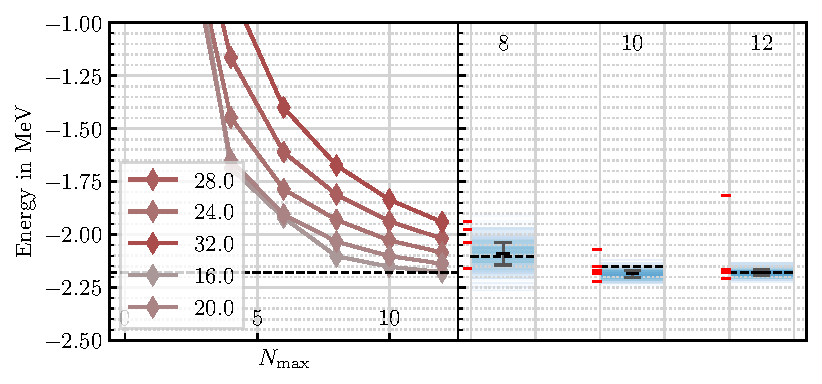
\includegraphics{media/outlook_selection.pdf}
  \caption{Evaluation of the \n{2}{H} nucleus in the difference based framework using only the three lowest frequencies. In this case, the frequencies are $\hbar\Omega = 16, 20, \SI{24}{\mega\electronvolt}$. The frequencies used in the evaluation are shown with solid lines. To achieve a better comparability to the previous extrapolations, the frequencies not taken into account are shown as dotted lines.}
  \label{fig:eval_freqselection}
\end{figure}

\section{Norming and monotonicity}
\input{chapters/8_outlook/further.tex}


\chapter{Conclusion}
\label{chap:conclusion}
In this thesis, we have formulated and analyzed two different extrapolation frameworks to predict the ground-state energy out of NCSM calculations using artificial neural networks.

In our first extrapolation framework (absolute-based), the input data consists of three different sequences of four NCSM calculations for consecutive $N_\mathrm{max}$ values. The output of the networks is then directly identified as the network prediction for the ground-state energy. In our second extrapolation framework (difference-based), we took the same sequences as described above and computed the difference of consecutive $N_\mathrm{max}$ values, resulting in three sequences of three values. In this case, the output is identified as the difference of the prediction and the mean absolute value at the largest $N_\mathrm{max}$. In both frameworks, the networks are trained according to that identification by the nuclei \n{2}{H}, \n{3}{H} and \n{4}{He} using chiral interactions of various leading orders and cutoffs for two-body interactions \cite{entemmachleidt} as well as two- and three-body interactions \cite{HUTHER2020135651}. Furthermore, the Hamiltonians were SRG evolved for flow parameters between \srg{0.04} and \srg{0.08}. To analyze the frameworks, we used the same nuclei with a semi-local momentum-space regulated N$^{2}$LO interaction with two-body interactions and a cutoff at \SI{450}{\mega\electronvolt} by Maris et. al \cite{smsquelle} which was SRG evolved using a flow parameter of \srg{0.04} and \srg{0.08}.

First, we have analyzed the extrapolation behavior of the absolute-based framework in dependency on the maximum $N_\mathrm{max}$ value of the used evaluation sequences and the SRG flow parameter. We have found two different systematic behaviors of the extrapolations for the nuclei \n{3}{H}, \n{4}{He} and the nucleus \n{2}{H}. The extrapolations for the nuclei \n{3}{H} and \n{4}{He} were generally too low and the networks corrected them to higher values with higher $N_\mathrm{max}$ values. For \n{2}{H}, the extrapolations were too high at low $N_\mathrm{max}$ values and got lower for higher $N_\mathrm{max}$. We have defined the variational boundary condition, which was satisfied for the extrapolations on \n{3}{H} and \n{4}{He} but not on \n{2}{H}. The classical extrapolations consisting of exponential function fits generally outperformed our framework on the more converged sequences of \n{3}{H} and \n{4}{He}, but were comparable for \n{2}{H}.

Before analyzing the difference-based framework, we discussed two different modifications on the training set for the absolute-based framework. The first modification consisted of restricting the training samples to a maximum $N_\mathrm{max}$ of $24$, while the second modification restricted the used interactions to SRG evolved interactions with a minimum flow parameter of \srg{0.04}. We have introduced the conditions of prediction consistency and reasonability to assess the two training modes. We have found that the $N_\mathrm{max}$-limitation training mode did not conform to those two conditions, while the SRG-filter training mode did. In general, the SRG-filter training mode produced the most promising extrapolations for our training nuclei.

After that, we have analyzed the previously introduced training modes in our difference-based framework. We have found that all of the training modes, as well as the unmodified training produced much more reasonable results for the nuclei. Here, the training modes did not significantly improve the value of the prediction but rather the uncertainty. As in the absolute-based framework, the SRG-filter training mode showed the most reasonable and consistent results.

In a real use-case application of our extrapolation framework using the nucleus \n{6}{Li}, which was previously unseen by the networks, we have seen that the SRG-filter training mode produced unreasonably high predictions while the $N_\mathrm{max}$-limitation training mode did not provide sufficiently different results to the unmodified training mode. The predictions of the unmodified training produced more consistent results than the classical extrapolations accross the $N_\mathrm{max}$ values. In a final decision using the insights of the extrapolation for all four nuclei, we have found the difference-based extrapolation framework together with the unmodified training to produce the overall most reasonable results.

Finally, we have looked into two different ideas that could further develop the difference-based framework to yield better results. The first idea included a new training modification, where frequencies were only included in the training if they are bigger or smaller than the frequency which results in the best convergence. The networks were thus trained to model the long or the short range of the nuclear interaction, respectively. We have found the high frequency filter training mode to produce more consistent and more precise results, although this idea has to be further examined for more nuclei. Secondly, we have persued the idea of manually selecting the frequencies for the evaluation data by choosing a selection rule. This results in better extrapolations, but limits the generality of our extrapolation framework.



\printbibliography
\end{document}
